%%%%%%%%%%%%%%%%%%%%%%%%%%%%%%%%%%%%%%%%%%%%%%%%%%%%%%%%%%%%%%%%%%%%%%%%%%%%%%
%  UHV-Complete.tex
%  Universal Human Values (HS248AT) -- the complete question bank.
%
%  One document combining:
%    Part I    descriptive question bank with model answers, unit-wise
%    Part II   objective question bank with answers
%    Part III  the nine past papers reproduced in full, dated and classified
%    Appendices  paper-to-answer index, repeats, revision priorities
%
%  Every answer is written strictly from the three prescribed unit notes
%  (A Foundation Course in Human Values and Professional Ethics, Chapters
%  1-10) and the official RVCE Scheme & Solution documents. Where a scheme
%  gives the model answer, that wording is followed.
%
%  Self-contained: standard CTAN packages only, no custom class required.
%  Build:  pdflatex UHV-Complete   (three times, for the TOC and links)
%%%%%%%%%%%%%%%%%%%%%%%%%%%%%%%%%%%%%%%%%%%%%%%%%%%%%%%%%%%%%%%%%%%%%%%%%%%%%%
\documentclass[11pt,a4paper,oneside]{book}

\usepackage[T1]{fontenc}
\usepackage[utf8]{inputenc}
\usepackage{lmodern}
\usepackage{microtype}
\usepackage[left=22mm,right=22mm,top=24mm,bottom=26mm,headsep=8mm]{geometry}
\usepackage[table]{xcolor}
\usepackage{enumitem}
\usepackage{titlesec}
\usepackage{fancyhdr}
\usepackage{booktabs}
\usepackage{longtable}
\usepackage{array}
\usepackage{needspace}
\usepackage{amssymb}
\usepackage{tikz}
\usetikzlibrary{arrows.meta,positioning,shapes.geometric,calc}
\usepackage[most]{tcolorbox}
\usepackage[hidelinks]{hyperref}

% ------------------------------------------------------------------- colours
\definecolor{ocre}{RGB}{243,102,25}
\definecolor{slate}{RGB}{45,55,72}
\definecolor{slatelight}{RGB}{113,128,150}
\definecolor{rulegrey}{RGB}{214,222,232}
\definecolor{tint}{RGB}{253,246,240}
\definecolor{panel}{RGB}{247,250,252}
\definecolor{tagbg}{RGB}{233,239,245}

\hypersetup{colorlinks=true, linkcolor=slate, urlcolor=ocre,
            pdftitle={Universal Human Values HS248AT -- The Complete Question
                      Bank with Answers},
            pdfsubject={IV Semester B.E., R V College of Engineering}}

% ---------------------------------------------------------------- structures
\newcolumntype{P}[1]{>{\raggedright\arraybackslash}p{#1}}
\newcolumntype{C}[1]{>{\centering\arraybackslash}p{#1}}

\setlength{\tabcolsep}{4pt}
\setlength{\arrayrulewidth}{0.4pt}

% ------------------------------------------------------------------ headings
\newcommand{\chapkind}{CHAPTER}

\titleformat{\part}[display]
  {\sffamily\bfseries\color{slate}}
  {\raggedright\normalsize\sffamily\color{ocre}PART \thepart}
  {8pt}
  {\Huge\raggedright}
  [\vspace{6pt}{\color{ocre}\rule{\textwidth}{2pt}}]
\titlespacing*{\part}{0pt}{0pt}{26pt}

\titleformat{\chapter}[display]
  {\sffamily\bfseries\color{slate}}
  {\raggedright\normalsize\sffamily\color{ocre}\chapkind\ \thechapter}
  {6pt}
  {\LARGE\raggedright}
  [\vspace{4pt}{\color{ocre}\rule{\textwidth}{1.6pt}}]
\titlespacing*{\chapter}{0pt}{-24pt}{18pt}

\newcommand{\qbsecbox}[1]{%
  \colorbox{slate}{\parbox{\dimexpr\textwidth-2\fboxsep\relax}%
    {\sffamily\bfseries\large\color{white}\strut #1\strut}}}
\titleformat{\section}[block]{}{}{0pt}{\qbsecbox}
\titlespacing*{\section}{0pt}{16pt}{8pt}

\titleformat{\subsection}[block]
  {\sffamily\bfseries\color{slate}\large}{}{0pt}{}
  [\vspace{-7pt}{\color{ocre}\rule{0.16\textwidth}{1pt}}]
\titlespacing*{\subsection}{0pt}{14pt}{4pt}

\pagestyle{fancy}
\fancyhf{}
\renewcommand{\headrulewidth}{0.4pt}
\fancyhead[L]{\footnotesize\sffamily\color{slatelight}HS248AT \textbullet\
  Universal Human Values}
\fancyhead[R]{\footnotesize\sffamily\color{slatelight}\leftmark}
\fancyfoot[C]{\footnotesize\sffamily\color{slatelight}\thepage}
\renewcommand{\chaptermark}[1]{\markboth{#1}{}}
\fancypagestyle{plain}{\fancyhf{}%
  \fancyfoot[C]{\footnotesize\sffamily\color{slatelight}\thepage}%
  \renewcommand{\headrulewidth}{0pt}}

% ------------------------------------------------------------- source tags
% a small pill naming a paper the question has actually appeared in
\newcommand{\tg}[1]{\,\colorbox{tagbg}{\scriptsize\sffamily\color{slate}%
  \strut\,#1\,}}
% the marks the source paper allotted
\newcommand{\mmk}[1]{\,{\footnotesize\sffamily\bfseries\color{ocre}#1\,M}}

% ---------------------------------------------------------- question heading
% \Q{number}{question text}{tag block}
\newcommand{\Q}[3]{%
  \needspace{6\baselineskip}%
  \vspace{9pt}%
  \noindent{\sffamily\bfseries\color{ocre}Q#1.}\enspace
  {\sffamily\bfseries\color{slate}#2}#3\par\vspace{2pt}}

% the "Ans." lead-in
\newcommand{\ans}{\noindent{\sffamily\bfseries\color{ocre}Ans.}\enspace}

% a pointer to another answer in this book
\newcommand{\seeq}[1]{\hspace{0.25em}{\footnotesize\sffamily\color{slatelight}%
  (see \textbf{Q#1})}}

% ------------------------------------------------------------------- lists
\newenvironment{apts}
  {\begin{enumerate}[label=\textbf{\color{ocre}\arabic*.},leftmargin=2.0em,
     itemsep=2pt,topsep=4pt,parsep=0pt]}
  {\end{enumerate}}
\newenvironment{abul}
  {\begin{itemize}[leftmargin=1.5em,itemsep=2pt,topsep=4pt,parsep=0pt,
     label=\textcolor{ocre}{\scriptsize$\blacksquare$}]}
  {\end{itemize}}
\newenvironment{alist}
  {\begin{enumerate}[label=\textbf{\color{ocre}(\alph*)},leftmargin=2.2em,
     itemsep=2pt,topsep=4pt,parsep=0pt]}
  {\end{enumerate}}

% a boxed note / caution
\newenvironment{note}
  {\begin{tcolorbox}[colback=tint,colframe=ocre,boxrule=0.8pt,sharp corners,
     fontupper=\small,breakable,before skip=8pt,after skip=8pt]}
  {\end{tcolorbox}}

% a quiet panel for definitions worth memorising verbatim
\newenvironment{keybox}
  {\begin{tcolorbox}[colback=panel,colframe=rulegrey,boxrule=0.8pt,
     sharp corners,fontupper=\small,breakable,
     before skip=7pt,after skip=7pt]}
  {\end{tcolorbox}}

% -------------------------------------------------------- generic table look
\newcommand{\hdr}[1]{{\sffamily\bfseries\color{white}\strut #1}}

% two-column comparison table
\newenvironment{cmptable}[2]
  {\renewcommand{\arraystretch}{1.3}\arrayrulecolor{rulegrey}%
   \setlength{\LTpre}{7pt}\setlength{\LTpost}{5pt}%
   \begin{longtable}{P{77mm} P{77mm}}
   \rowcolor{slate}\hdr{#1} & \hdr{#2} \\ \hline \endfirsthead
   \rowcolor{slate}\hdr{#1} & \hdr{#2} \\ \hline \endhead}
  {\end{longtable}}

% ------------------------------------------------------ exam-paper question grid
\newenvironment{qtable}
  {\renewcommand{\arraystretch}{1.28}%
   \arrayrulecolor{rulegrey}%
   \setlength{\LTpre}{6pt}\setlength{\LTpost}{4pt}%
   \begin{longtable}{C{10mm} P{95mm} C{9mm} C{11mm} C{8mm} C{13mm}}
   \rowcolor{slate}
   \hdr{Q.\,No} & \hdr{Question} & \hdr{M} & \hdr{CO} & \hdr{BT} & \hdr{Answer}
   \\ \hline \endfirsthead
   \rowcolor{slate}
   \hdr{Q.\,No} & \hdr{Question} & \hdr{M} & \hdr{CO} & \hdr{BT} & \hdr{Answer}
   \\ \hline \endhead}
  {\end{longtable}}

\newcommand{\qn}[1]{{\sffamily\bfseries\color{ocre}#1}}
% pointer into Parts I / II
\newcommand{\ap}[1]{{\sffamily\bfseries\color{slate}\small #1}}
\newcommand{\orband}{\multicolumn{6}{c}{\cellcolor{tint}%
  \sffamily\bfseries\color{ocre}\strut OR} \\ \hline}
\newcommand{\blank}{\underline{\hspace{2.6em}}}
\newcommand{\optsinline}[4]{\par\vspace{3pt}%
  {\small\color{slate}(a)~#1\quad (b)~#2\quad (c)~#3\quad (d)~#4}}
\newenvironment{optlist}
  {\par\vspace{2pt}\begingroup\small\color{slate}%
   \begin{enumerate}[label={\color{slatelight}(\alph*)},leftmargin=2.0em,
     itemsep=1pt,topsep=2pt,parsep=0pt]}
  {\end{enumerate}\endgroup\vspace{1pt}}

% paper metadata panel
\newenvironment{papermeta}
  {\begin{tcolorbox}[colback=panel,colframe=rulegrey,boxrule=0.8pt,
     sharp corners,left=8pt,right=8pt,top=7pt,bottom=7pt,
     before skip=4pt,after skip=10pt]
   \renewcommand{\arraystretch}{1.25}%
   \begin{tabular}{@{}P{24mm}P{48mm}@{\hspace{6mm}}P{24mm}P{46mm}@{}}}
  {\end{tabular}\end{tcolorbox}}
\newcommand{\mk}[1]{{\footnotesize\sffamily\bfseries\color{slatelight}%
  \MakeUppercase{#1}}}
\newcommand{\mv}[1]{{\color{slate}#1}}

% marks-distribution footer table
\newenvironment{mdtable}
  {\renewcommand{\arraystretch}{1.3}\arrayrulecolor{rulegrey}%
   \begin{tabular}{@{}P{38mm} C{11mm}C{11mm}C{11mm}C{11mm}
                        C{9mm}C{9mm}C{9mm}C{9mm}C{9mm}C{9mm}@{}}
   \rowcolor{slate}
   \hdr{Particulars} & \hdr{CO1} & \hdr{CO2} & \hdr{CO3} & \hdr{CO4} &
   \hdr{L1} & \hdr{L2} & \hdr{L3} & \hdr{L4} & \hdr{L5} & \hdr{L6}
   \\ \hline}
  {\end{tabular}}

% objective question grid (Part II)
\newenvironment{objtable}
  {\renewcommand{\arraystretch}{1.3}\arrayrulecolor{rulegrey}%
   \setlength{\LTpre}{7pt}\setlength{\LTpost}{5pt}%
   \begin{longtable}{C{8mm} P{99mm} P{45mm}}
   \rowcolor{slate}\hdr{\#} & \hdr{Question} & \hdr{Answer}
   \\ \hline \endfirsthead
   \rowcolor{slate}\hdr{\#} & \hdr{Question} & \hdr{Answer}
   \\ \hline \endhead}
  {\end{longtable}}

% index grid used in the appendices
\newenvironment{idxtable}
  {\renewcommand{\arraystretch}{1.3}\arrayrulecolor{rulegrey}%
   \setlength{\LTpre}{6pt}\setlength{\LTpost}{4pt}%
   \begin{longtable}{C{13mm} P{110mm} C{12mm} C{16mm}}
   \rowcolor{slate}
   \hdr{Q} & \hdr{Question} & \hdr{Marks} & \hdr{See}
   \\ \hline \endfirsthead
   \rowcolor{slate}
   \hdr{Q} & \hdr{Question} & \hdr{Marks} & \hdr{See}
   \\ \hline \endhead}
  {\end{longtable}}

\setlength{\parindent}{0pt}
\setlength{\parskip}{3pt}
\setlength{\emergencystretch}{3em}

%%%%%%%%%%%%%%%%%%%%%%%%%%%%%%%%%%%%%%%%%%%%%%%%%%%%%%%%%%%%%%%%%%%%%%%%%%%%%%
\begin{document}
\frontmatter
\pagestyle{empty}

% ---------------------------------------------------------------- title page
\begin{center}
\vspace*{28mm}
{\sffamily\color{ocre}\large HS248AT \textbullet\ IV SEMESTER B.E.}\\[3mm]
{\color{rulegrey}\rule{0.55\textwidth}{1pt}}\\[9mm]
{\sffamily\bfseries\color{slate}\Huge UNIVERSAL HUMAN VALUES}\\[7mm]
{\sffamily\bfseries\color{slate}\LARGE The Complete Question Bank}\\[3mm]
{\sffamily\color{slatelight}\Large with Model Answers, and every past paper
 reproduced in full}\\[12mm]
{\color{rulegrey}\rule{0.55\textwidth}{1pt}}\\[9mm]
{\sffamily\color{slate}\large Units I, II and III \textbullet\ Chapters 1 to
 10 \textbullet\ 150 questions}\\[3mm]
{\sffamily\color{slatelight}\large Nine papers \quad\textbullet\quad
 October 2023 to June 2026}\\[16mm]
{\sffamily\color{slatelight} Department of Industrial Engineering and
 Management}\\[1mm]
{\sffamily\color{slatelight} R V College of Engineering, Bengaluru}\\
\vfill
{\footnotesize\sffamily\color{slatelight}
 Unofficial student-compiled study material. Not issued, endorsed or verified
 by the Department or by RV College of Engineering.}
\vspace*{10mm}
\end{center}
\clearpage

% ---------------------------------------------------------------------------
%  How this book is arranged
% ---------------------------------------------------------------------------
\chapter*{How This Book Is Arranged}
\addcontentsline{toc}{chapter}{How This Book Is Arranged}
\markboth{How This Book Is Arranged}{}
\thispagestyle{plain}

This is the whole of HS248AT in one document: every question recorded for the
course --- \textbf{150 in all} --- answered, plus every paper those questions
came from, reproduced as it was set.

\vspace{2pt}
It is in three parts, because there are three different ways you will want to
use it.

\begin{abul}
\item \textbf{Part I --- the descriptive question bank.} Every long-answer
      question ever set, arranged \emph{unit-wise} against the syllabus, each
      with a model answer. This is the part you revise from. Reading it
      straight through covers the course; \textbf{74 questions}.
\item \textbf{Part II --- the objective question bank.} Every multiple-choice
      question, fill-in-the-blank and one-mark short answer, with the answer
      beside it. \textbf{76 items}, in three tables --- 36 multiple-choice,
      35 fill-in-the-blank, 5 short answers.
\item \textbf{Part III --- the question papers.} All nine papers reproduced in
      full and in chronological order, with the date, assessment type,
      duration, maximum marks and the printed instructions. Every question
      carries a pointer to its answer in Part~I or Part~II, so a whole past
      paper can be worked end to end and then marked.
\end{abul}

The two arrangements are deliberate. Part~I is arranged by topic because
that is how you learn; Part~III is arranged by paper because that is how you
are examined, and a paper's shape --- how many marks Part~A carries, which
questions offer a choice --- is itself worth knowing before you sit down.

\subsection*{Where the answers come from}
\addcontentsline{toc}{section}{Where the answers come from}

Every answer in this book is written \textbf{strictly from the prescribed
material and nothing else}: the three unit notes for this course (\emph{A
Foundation Course in Human Values and Professional Ethics}, Chapters 1--10),
and the official RVCE \emph{Scheme \& Solution} documents for CIE~2 (2022--23)
and Quiz-3\,/\,CIE~3 (2023--24). Where a scheme gives the model answer, that
wording is followed in substance.

Nothing has been imported from outside those sources. Where a past-paper
question uses a term the notes do not define in that form, the answer says so
and answers from the nearest thing the notes do define, rather than filling
the gap from elsewhere.

\begin{note}
\textbf{\sffamily Two warnings about circulating answer-sets.}

\textbf{(1) Justice.} The Unit~II answer-set circulating as ``unit-2 uhv
question bank answers'' defines justice using the legal categories
\emph{distributive\,/\,procedural\,/\,retributive\,/\,restorative}. That
contradicts the official RVCE scheme, which defines the four elements of
justice as \emph{recognition of values, fulfilment, evaluation,} and
\emph{mutual happiness ensured}. This book follows the official scheme and the
prescribed text throughout --- write those in the exam.

\textbf{(2) Chapters 11--13.} Two SEE questions (\emph{holistic technology};
\emph{ethical human conduct in terms of values, policy and character}) belong
to Chapters 11--13, which are not part of the Unit I--III material supplied.
They are listed in the paper index but not answered here, since no source was
provided for them. That omission is flagged where it occurs rather than
papered over.
\end{note}

\subsection*{Reading the tags}
\addcontentsline{toc}{section}{Reading the tags}

Each question in Part~I carries a tag block naming the papers it has actually
appeared in, and the marks the source paper allotted:

\vspace{4pt}
\begin{keybox}
\textbf{Q32.}\enspace What do you understand by trust? Differentiate between
intention and competence.\tg{CIE 2}\tg{SEE}\mmk{5}

\vspace{5pt}
{\footnotesize This question was set in a CIE~2 paper and in an SEE, and
carried 5 marks. A question tagged with three or four papers is the single
best use of revision time --- Appendix~B lists them all.}
\end{keybox}

\vspace{4pt}
\tg{Scheme} means the answer follows the official RVCE scheme verbatim in
substance. An untagged question has not yet appeared in a paper we hold; it is
in the book because the departmental question bank or the notes' own review
questions set it, and it covers syllabus the papers have so far skirted.

In Part~III every question additionally carries the three codes its paper
printed beside it --- \textbf{M} (marks), \textbf{CO} (course outcome, code
only) and \textbf{BT} (Bloom's level, \textbf{L1} remember, \textbf{L2}
understand, \textbf{L3} apply, \textbf{L4} analyse). No paper in this
collection sets anything above L4.

\subsection*{The nine papers}
\addcontentsline{toc}{section}{The nine papers}

\renewcommand{\arraystretch}{1.35}
\arrayrulecolor{rulegrey}
\begin{tabular}{@{}P{46mm} P{32mm} C{20mm} C{20mm} C{28mm}@{}}
\rowcolor{slate}
\hdr{Assessment} & \hdr{Date} & \hdr{Max M} & \hdr{Time} & \hdr{Reproduced} \\
\hline
SEE (21HSU48) & October 2023 & 50 & 2 h & Index only \\ \hline
CIE 1 & 22 June 2024 & 25 & 60 min & Index only \\ \hline
CIE 2 & 24 July 2024 & 5 + 25 & 60 min & Index only \\ \hline
Improvement CIE\,/\,CIE 3 & 28 August 2024 & 25 & 60 min &
  \textbf{Part III} \\ \hline
SEE & Sept/Oct 2024 & 50 & 2 h & Index only \\ \hline
CIE-II & 7 May 2025 & 25 + 5 & 60 min & \textbf{Part III} \\ \hline
Improvement CIE & June 2025 & 30 & 60 min & \textbf{Part III} \\ \hline
\textbf{SEE} Regular\,/\,Suppl. & June/July 2025 & 50 & 2 h &
  \textbf{Part III} \\ \hline
Improvement CIE & 18 June 2026 & 05 + 25 & 10 + 60 min &
  \textbf{Part III} \\ \hline
\end{tabular}

\vspace{6pt}
Five papers are reproduced question-for-question in Part~III because scans of
the full papers were available. For the other four only the question list
survives, so they appear in the Appendix~A index --- but every one of their
questions is answered in Parts~I and~II just the same. Nothing has been
dropped for want of a scan.

\subsection*{How long an answer should be}
\addcontentsline{toc}{section}{How long an answer should be}

Answers here are written to the length the marks buy. The valuation scheme for
this course awards roughly one mark per distinct, correctly explained point,
so a 5-mark answer carries five scoring points, a 6-mark answer six, an 8-mark
answer eight. A 4-mark definition question is two to four sentences.

In the examination you are not rewarded for volume. You are rewarded for
hitting the number of distinct points the scheme expects, each named and then
explained in a line or two. Where an answer below runs longer than you could
write in the time available, treat the \textbf{numbered points as the skeleton
to reproduce} and the prose as the explanation to compress.

\vspace{4pt}
Appendix~C lists, unit by unit, what to revise first if you have run out of
time.


\clearpage
\tableofcontents

\mainmatter
\pagestyle{fancy}

\part{Descriptive Question Bank with Answers}
% ---------------------------------------------------------------------------
%  UNIT I -- Chapters 1 to 7
% ---------------------------------------------------------------------------
\chapter{Unit I --- Value Education, Self-exploration, Basic Human
  Aspirations and Harmony in the Self}
\chaptermark{Unit I --- Chapters 1 to 7}

\section{A. Understanding Value Education (Chapter 1)}

% ------------------------------------------------------------------------- 1
\Q{1}{What do you mean by values or human values? What is value education,
  and why is it needed?}{\tg{SEE}\mmk{6}}

\ans Character-oriented education that instils basic values and ethical value
in one's psyche is called \textbf{value-based education}. The subject that
enables us to understand `what is valuable' for human happiness is called
\textbf{value education}.

Values form the basis for all our thoughts, behaviour and actions. Once we
know what is valuable to us, these values become the basis, the anchor, for
our actions. Value education is important to help everyone improve the value
system he\,/\,she holds and put it to use. Once one has understood one's
values in life, one can examine and control the various choices one makes.

Value education enables us to understand our needs and visualise our goals
correctly, indicates the direction for their fulfilment, helps remove our
confusions and contradictions, brings harmony at all levels, and enables us to
rightly utilise technological innovations. We also need to understand the
universality of various human values, because only then can we have a definite
and common programme for value education --- and only then can we be assured
of a happy and harmonious human society.

% ------------------------------------------------------------------------- 2
\Q{2}{What is the need for value education? Explain its five
  aspects.}{\tg{SEE}\mmk{6}}

\ans
\begin{apts}
\item \textbf{Correct identification of our aspirations.} All human beings
      have aspirations and make plans. Before investing energy in actualising
      those plans, it is important to find out what we basically aspire for.
      Value education enables us to understand our needs, visualise our goals
      correctly and indicate the direction for their fulfilment.
\item \textbf{Understanding universal human values to fulfil our aspirations
      in continuity.} Identifying the aspiration is not enough; we must know
      how to fulfil it. Generally we pursue goals as per our appraisal and
      beliefs. Complete understanding of human values gives us a definite way
      to fulfil our aspirations.
\item \textbf{Complementarity of values and skills.} First we must know what
      really is conducive to human happiness --- happiness for one and for
      all, and at all times. This is the \emph{value domain}, the domain of
      wisdom. Secondly, we must learn methods and practices to actualise this
      goal in real life --- this is the \emph{domain of skills}. Both must go
      hand in hand.
\item \textbf{Evaluation of our beliefs.} In the absence of a correct
      understanding of universal human values we are driven by ad-hoc values
      and beliefs, which may or may not be true in reality. These beliefs come
      from what we read, see and hear, what our parents tell us, what
      magazines and TV say. They keep changing with time and are often
      mutually conflicting. Value education helps us evaluate our beliefs and
      assumed values.
\item \textbf{Technology and human values.} Technology is only a means to
      achieve what is considered valuable. It is not within the scope of
      technology to decide what is valuable --- that decision lies outside it.
      Without this decision technology can be aimless and can be put to any
      use, constructive or destructive. Hence technical education must be
      supplemented with value education.
\end{apts}

Value education is a crucial missing link in the present education system.
Because of this deficiency, most of our efforts may prove counterproductive,
and serious crises at the individual, societal and environmental level are
manifesting.

% ------------------------------------------------------------------------- 3
\Q{3}{What are the basic guidelines for value education?}{\tg{SEE}\mmk{6}}

\ans To qualify as an appropriate input in value education, the content of the
course must satisfy the following guidelines:

\begin{abul}
\item \textbf{Universal.} It must be applicable to all human beings
      irrespective of caste, creed, gender, nationality or religion, and be
      true at all times and all places.
\item \textbf{Rational.} It must appeal to human reasoning --- amenable to
      reasoning, and not based on dogmas or blind beliefs. It cannot be a set
      of sermons or do's and don'ts.
\item \textbf{Natural and verifiable.} It must be naturally acceptable to the
      human being who goes through the course, and living on the basis of such
      values must lead to fulfilment and happiness. It must be experientially
      verifiable and not based on dogmas, beliefs or assumptions.
\item \textbf{All-encompassing.} Value education is aimed at transforming our
      consciousness and living. Hence it must cover all the dimensions
      (thought, behaviour, work and realisation) and all the levels
      (individual, family, society, nature and existence) of human life and
      profession.
\item \textbf{Leading to harmony.} It must ultimately promote harmony within
      the individual, among human beings, and with the rest of nature.
\end{abul}

% ------------------------------------------------------------------------- 4
\Q{4}{What do you understand by the value of an entity? What is the value of
  a human being?}{\tg{SEE 2025}\mmk{4--8}}

\ans \textbf{The value of any unit in this existence is its participation in
the larger order of which it is a part.} For example, the value of a pen is
that it can write --- here writing is the participation of the pen in the
bigger order in which pen, paper and human being are all present. The value of
an eye is that it can be used for seeing. The value of a vegetable plant is
that it gives nutrition to animals and humans.

The \textbf{value of a human being} is the participation of the human being at
different levels in this order. This participation is seen in two forms ---
\emph{behaviour} and \emph{work}. The participation pertaining to behaviour
consists of the nine values in relationship: trust, respect, affection, care,
guidance, reverence, glory, gratitude and love. Working with material things,
we have two values: \textbf{utility value} and \textbf{artistic value}. All
these values are nothing but the participation of the human being in different
dimensions of living.

\begin{keybox}
\textbf{\sffamily Note for the 8-mark SEE version.} This question was set for
8 marks in June/July 2025 (Q2a). At that length, define the value of an
entity, give three examples, then give the value of a human being in
\emph{both} its forms --- the nine values in behaviour, named, and the two
values in work --- and close by stating that value is participation, not a
property the thing owns by itself.
\end{keybox}

% ------------------------------------------------------------------------- 5
\Q{5}{Illustrate the content of value education. What should its scope
  be?}{\mmk{5}}

\ans The scope of value education includes \textbf{all dimensions} (thought,
behaviour, work and realisation) and \textbf{all levels} (individual, family,
society, nature\,/\,existence) of human living.

Accordingly, the content of value education is: to understand myself, my
aspirations and my happiness; to understand the goal of human life
comprehensively; to understand the other entities in nature, the innate
interconnectedness and the co-existence in nature\,/\,existence; and finally
the role of the human being in this nature\,/\,existence entirely. Hence it
has to encompass the understanding of harmony at various levels ---
individual, family, society, nature and existence --- and finally, learning to
live in accordance with this understanding by being vigilant to one's thought,
behaviour and work.

% ------------------------------------------------------------------------- 6
\Q{6}{What do you mean by values? How do they differ from skills? How are
  values and skills complementary? Give two examples.}{\tg{SEE}\mmk{6}}

\ans \textbf{Values} mean importance or participation --- knowing what really
is conducive to human happiness, happiness for one and for all and at all
times. This is the \emph{value domain}, the domain of wisdom; it helps us
identify and set the right goals and proceed in the right direction.
\textbf{Skills} mean the qualities, training and capabilities --- the methods,
practices and techniques to actualise that goal in real life, in various
dimensions of human endeavour. This is the \emph{domain of skills}.

To fulfil our aspirations, both are necessary; hence there is an essential
complementarity between values and skills for the success of any human
endeavour.

\textbf{Example 1 (health).} I want to lead a healthy life. Only wishing for
good health will not keep my body fit; and without having understood the
meaning of health, I will not be able to choose things correctly to keep my
body fit. So I have to learn the skills to achieve the goal of good health ---
what food to consume, what physical workout to design. Without knowing the
meaning of good health (value), health cannot be achieved; and without the
skill, the goal cannot be reached.

\textbf{Example 2 (technology).} If we value the relationship with the
environment, we will work to create environment-friendly technologies (the
structure of technology) and also put them to right use (use of technology)
--- say for the enrichment of the environment and replenishment of natural
resources. The engineering skill produces the technology; the value decides
what to produce and how to use it. Conversely, if the relationship with the
environment is something we do not value, things could be the other way round.

% ------------------------------------------------------------------------- 7
\Q{7}{What is the need for value education in technical and other
  professional institutions?}{\mmk{5}}

\ans The present education system has become largely skill-based; the prime
emphasis is on science and technology, and on the skills to apply them. There
is very little in it that helps a student decide \emph{what is worth doing
with} those skills.

\begin{abul}
\item An engineer's decisions have consequences far beyond the engineer ---
      on other people, on society and on nature. Deciding what to produce,
      and how it should be used, is a question in the value domain, not the
      skill domain. Technology cannot answer it.
\item Without value education, professional competence is left aimless. The
      same competence can be put to constructive or destructive use, and
      nothing in the technical syllabus itself distinguishes the two.
\item Professionals with right understanding can ensure that their
      professional competence leads to mutual fulfilment in relationship and
      mutual prosperity with the rest of nature, rather than to exploitation
      of either.
\item The problems at the level of the individual, family, society and nature
      that we see today are a direct outcome of an incorrect understanding of
      happiness and prosperity, not of a shortage of technical skill. They
      cannot be solved by more skill alone.
\item Hence technical education must be \emph{supplemented} --- not replaced
      --- by value education, so that values and skills go hand in hand.
\end{abul}

\section{B. Self-exploration as the Process for Value Education (Chapter 2)}

% ------------------------------------------------------------------------- 8
\Q{8}{Define self-exploration. What is the content of
  self-exploration?}{\tg{CIE 1}\mmk{5}}

\ans \textbf{Self-exploration is the process of finding out what is valuable
to me by investigating within myself.} Since it is I who feels happy or
unhappy, successful or unsuccessful, whatever is right for me, true for me,
has to be judged within myself. Through self-exploration we get the value of
ourselves. We live with an entirety --- family, friends, air, soil, water,
trees --- and we want to understand our relationship with all these; for this
we need to start observing inside.

The main focus of self-exploration is \textbf{myself --- the human being}. Its
content is finding answers to the following two fundamental questions of all
human beings:

\begin{apts}
\item \textbf{Desire\,/\,Goal:} What is my (human) desire or goal? What do I
      really want in life, or what is the goal of human life?
\item \textbf{Programme:} What is my (human) programme for fulfilling the
      desire? What is the process to fulfil this basic aspiration?
\end{apts}

In short, these two questions cover the whole domain of human aspiration and
human endeavour; thus they form the content of self-exploration.

% ------------------------------------------------------------------------- 9
\Q{9}{Explain the process of self-exploration with a
  diagram.}{\tg{SEE}\mmk{6}}

\ans The process of self-exploration has to be kept in mind as follows:

\begin{abul}
\item \textbf{Whatever is being presented is a PROPOSAL.} Don't start by
      assuming it to be true or false.
\item \textbf{Verify it in your own right} --- not on the basis of scriptures,
      not on the basis of readings from instruments, and not on the basis of
      the assertion of other human beings.
\item \textbf{Firstly, verify the proposal on the basis of your natural
      acceptance.} Natural acceptance is a faculty present in each one of us;
      it is intact and invariant. We only have to start paying attention to
      it. (E.g. ask yourself: \emph{Is trust naturally acceptable to me in
      relationship, or is mistrust?} The answer comes from within,
      spontaneously.)
\item \textbf{Secondly, live according to the proposal to validate it
      experientially.} If the proposal is true, then in behaviour with other
      humans it will lead to \emph{mutual fulfilment\,/\,mutual happiness},
      and in work with the rest of nature it will lead to \emph{mutual
      prosperity}.
\end{abul}

\vspace{6pt}
\begin{center}
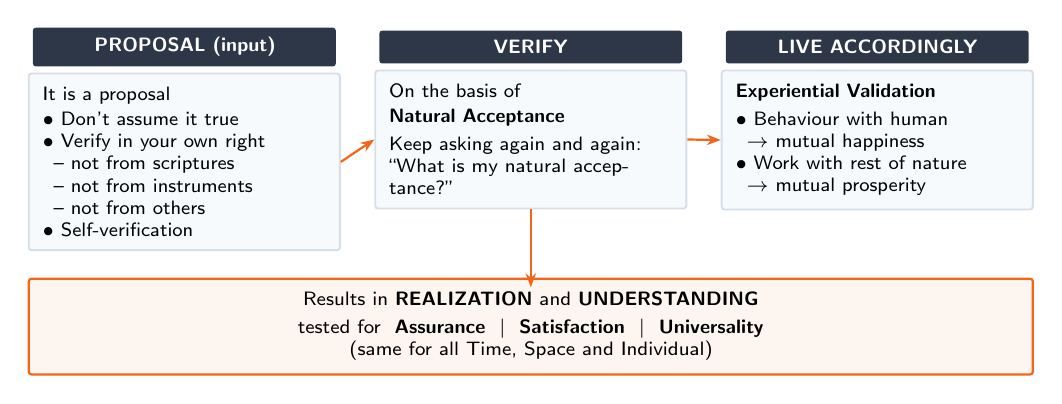
\begin{tikzpicture}[
  font=\sffamily\scriptsize,
  box/.style={draw=rulegrey,fill=panel,rounded corners=1pt,line width=0.7pt,
              align=left,inner sep=5pt,text width=36mm},
  head/.style={draw=none,fill=slate,text=white,rounded corners=1pt,
               align=center,inner sep=3.5pt,text width=36mm,font=\sffamily\bfseries\scriptsize},
  res/.style={draw=ocre,fill=tint,rounded corners=1pt,line width=0.8pt,
              align=center,inner sep=5pt,text width=124mm},
  ar/.style={-{Stealth[length=5pt]},line width=0.8pt,draw=ocre}]

\node[head] (h1) at (0,0) {PROPOSAL (input)};
\node[head] (h2) at (4.4,0) {VERIFY};
\node[head] (h3) at (8.8,0) {LIVE ACCORDINGLY};

\node[box,below=2pt of h1,text width=36mm] (b1)
  {It is a proposal\\[1pt]
   $\bullet$ Don't assume it true\\
   $\bullet$ Verify in your own right\\
   \hspace*{4pt}-- not from scriptures\\
   \hspace*{4pt}-- not from instruments\\
   \hspace*{4pt}-- not from others\\
   $\bullet$ Self-verification};
\node[box,below=2pt of h2,text width=36mm] (b2)
  {On the basis of\\[1pt]
   \textbf{Natural Acceptance}\\[2pt]
   Keep asking again and again:\\
   ``What is my natural acceptance?''};
\node[box,below=2pt of h3,text width=36mm] (b3)
  {\textbf{Experiential Validation}\\[2pt]
   $\bullet$ Behaviour with human\\
   \hspace*{4pt}$\rightarrow$ mutual happiness\\
   $\bullet$ Work with rest of nature\\
   \hspace*{4pt}$\rightarrow$ mutual prosperity};

\draw[ar] (b1.east) -- (b2.west);
\draw[ar] (b2.east) -- (b3.west);

\node[res] at (4.4,-3.55)
  {Results in \textbf{REALIZATION} and \textbf{UNDERSTANDING}\\[2pt]
   tested for \ \textbf{Assurance} \ $\vert$ \ \textbf{Satisfaction} \
   $\vert$ \ \textbf{Universality}\\
   (same for all Time, Space and Individual)};
\draw[ar] (b2.south) -- (4.4,-3.05);
\end{tikzpicture}
\end{center}

The answers we get on having realisation and understanding are:
\textbf{(a) Assuring} --- ``I am assured of the answer in myself'';
\textbf{(b) Satisfying} --- ``I am satisfied that the answers are fulfilling
for me''; \textbf{(c) Universal} --- the answers are the same for everyone,
invariant with respect to time, space and individual. If the answer fails any
of these criteria, it is most likely coming from past beliefs or conditioning
and not from natural acceptance, and needs to be re-verified.

% ------------------------------------------------------------------------ 10
\Q{10}{What do you mean by natural acceptance and experiential validation?
  Explain them as the two mechanisms of self-exploration.}{\tg{SEE}\mmk{5}}

\ans \textbf{Natural acceptance} implies unconditional and total acceptance of
the self, people and environment; it also refers to the absence of any
exception from others. It is a faculty present in each one of us, intact and
invariant, and we can always refer to it to know what is right for us. Once we
fully and truly commit ourselves on the basis of natural acceptance, we feel a
holistic sense of inner harmony, tranquillity and fulfilment.

\textbf{Experiential validation} is the process that infuses direct experience
with the learning environment and content. It may be regarded as a philosophy
and methodology in which the direct experience and focused reflection of the
individual helps to increase knowledge, develop skill and clarify values. We
live according to the proposal, and if it is true, our behaviour with humans
leads to mutual happiness and our work with the rest of nature leads to mutual
prosperity. When what we already believe to be true of us is validated by
situations, phenomena or outcomes, we may term it experiential validation.

Self-exploration takes place in \textbf{the Self, and not in the body}.

% ------------------------------------------------------------------------ 11
\Q{11}{Illustrate the purpose of self-exploration. (Seven points)}{\mmk{5}}

\ans
\begin{apts}
\item \textbf{It is a process of dialogue between ``what you are'' and ``what
      you really want to be''.} If these two are the same, there is no
      problem. If on investigation we find they are not the same, we are
      living with this contradiction, and we need to resolve this conflict
      within us.
\item \textbf{It is a process of self-evolution through self-investigation.}
      It successively enables us to bridge the gap between `what we are' and
      `what we want to be'; we become qualitatively better.
\item \textbf{It is a process of knowing oneself and, through that, knowing
      the entire existence.} The exploration starts by asking simple questions
      about ourselves, which gives clarity about our being, and then clarity
      about everything around us.
\item \textbf{It is a process of recognising one's relationship with every
      unit in existence and fulfilling it.} We become aware of our right
      relationship with other entities, discover the interconnectedness and
      co-existence, and live accordingly.
\item \textbf{It is a process of knowing human conduct, human character and
      living accordingly.} We all desire certainty and stability; once we know
      our own true nature, we understand our participation with the other
      things we live with --- this is the ethical or humane conduct.
\item \textbf{It is a process of being in harmony in oneself and in harmony
      with the entire existence.}
\item \textbf{It is a process of identifying our innateness and moving towards
      self-organisation and self-expression.}
\end{apts}

\begin{center}
{\sffamily\bfseries\color{slate}Svatva \ $\rightarrow$ \ Swatantrata \
 $\rightarrow$ \ Swarajya}
\end{center}

% ------------------------------------------------------------------------ 12
\Q{12}{What do you understand by the terms svatva, swatantrata and swarajya?
  How are they related?}{\mmk{5}}

\ans
\begin{abul}
\item \textbf{Svatva (innateness):} the innateness of the self --- the natural
      acceptance of harmony.
\item \textbf{Swatantrata (self-organisation):} being self-organised --- being
      in harmony with oneself.
\item \textbf{Swarajya (self-expression):} self-expression, self-extension ---
      living in harmony with others, and thus participation towards harmony in
      the whole existence.
\end{abul}

\begin{center}
{\sffamily\bfseries\color{slate}Svatva \ $\rightarrow$ \ Swatantrata \
 $\rightarrow$ \ Swarajya}
\end{center}

The \emph{svatva} is already there, intact in each one of us. By being in
dialogue with it, we attain \emph{swatantrata}, which enables us to work for
\emph{swarajya}. If we live in contradiction, it means we are not
self-organised and are living with pre-conditionings, having assumed certain
things and accumulated desires without first evaluating them --- then we are
\emph{partantra} (enslaved). On the other hand, when we identify our
innateness, what we really want to be, and establish a dialogue with it, it
enables us to start living with this harmony; it starts expressing itself
through our harmonious behaviour and work, and naturally extends to our
participation with the surroundings. This is working towards \emph{swarajya}.

% ------------------------------------------------------------------------ 13
\Q{13}{``Natural acceptance is innate, invariant and universal.'' Explain
  this statement with an example.}{\mmk{5}}

\ans We can verify proposals on the basis of the following characteristics of
natural acceptance:

\begin{apts}
\item \textbf{Natural acceptance does not change with time.} It remains
      invariant with time. For example, our natural acceptance for trust and
      respect does not change with age; people a hundred years ago also had
      the same natural acceptance.
\item \textbf{It does not depend on the place.} Whether we are in New Delhi,
      New York or Abu Dhabi, if we address our natural acceptance the answer
      would still be the same.
\item \textbf{It does not depend on our beliefs or past conditionings.} No
      matter how deep our belief or past conditioning, as long as we ask
      ourselves the question sincerely and refer deep within ourselves, the
      answer will always be the same.
\item \textbf{This natural acceptance is `constantly there', something we can
      refer to.} Try it: think of cheating or exploiting someone. The moment
      you think of this, you sense a contradiction within and feel unhappy
      that very instant. Every time we do something not acceptable to us,
      there is a contradiction in us, because the thought or deed conflicts
      with our own natural acceptance.
\item \textbf{Natural acceptance is the same for all of us.} It is part and
      parcel of every human being; it is part of human-ness. No human being
      finds disrespect acceptable in relationship. Our assumptions and
      choices, likes and dislikes may be different, but on basic and common
      issues like the need to be happy, to be respected, to be prosperous, we
      are all the same.
\end{apts}

\textbf{Example.} Take the proposal --- `respect is a value in human
relation'. When I verify at the level of natural acceptance, I find that it is
naturally acceptable to me. Similarly, when I behave with respect, it is
mutually fulfilling to me and to the other. Thus the proposal is true. If it
fails either of the two tests, it is untrue.

\section{C. The Basic Human Aspirations (Chapter 3)}

% ------------------------------------------------------------------------ 14
\Q{14}{What is happiness? ``To be in a state of harmony is happiness'' ---
  explain and illustrate with two examples from your day-to-day
  life.}{\tg{SEE}\mmk{6}}

\ans Happiness may be defined as \textbf{being in harmony\,/\,synergy in the
state or situation that I live in}.

\begin{keybox}
``The state\,/\,situation in which I live, if there is harmony\,/\,synergy in
it, then I like to be in that state\,/\,situation.'' \quad i.e. \quad
\textbf{To be in a state of liking is happiness.}

\vspace{3pt}
Conversely: ``The state\,/\,situation in which I live, if there is
conflict\,/\,contradiction in it, then I do not like to be in that state or
situation'' --- \textbf{to be in a state of disliking is unhappiness}.
\end{keybox}

Thus, \textbf{to be in a state of harmony is happiness; to be in a state of
disharmony or contradiction is unhappiness.} When we are in such a state of
happiness we experience no struggle, no contradiction or conflict within, and
we wish to have its continuity. One important characteristic of this feeling
is that \emph{we like to continue it}.

\textbf{Example 1 --- Respect.} Respect is a state of harmony between two
human beings. When I respect the other and the other respects me, I like to be
in that situation; it gives me happiness.

\textbf{Example 2 --- Harmony in my own thoughts.} When there is harmony in my
thoughts and feelings, I feel relaxed and want to be in that situation. This
feeling is happiness. If this harmony is disturbed --- say I am confused or in
conflict about a decision --- I feel uneasy, i.e. unhappy.

It should be noted that we do get an impression of happiness through sensory
interaction (tasty food, a beautiful picture, a sweet fragrance). However,
these impressions are always short-lived and their continuity can never be
ensured.

% ------------------------------------------------------------------------ 15
\Q{15}{What is the meaning of prosperity? How can you say that you are
  prosperous?}{\mmk{5}}

\ans \textbf{Prosperity is the feeling of having or making available more than
the required physical facilities.} Physical facilities are the material things
we use to fulfil the needs of the body; when we are able to cater to the needs
of the body adequately, we feel prosperous.

To ascertain prosperity, \textbf{two things} are essential:

\begin{apts}
\item \textbf{Correct assessment of the need for physical facilities} ---
      identification of the required quantity. We can be prosperous only if
      there is a limit to the need for physical facilities. If there is no
      limit, then whatsoever be the availability with us, the feeling of
      prosperity cannot be assured.
\item \textbf{The competence of making available more than the required
      physical facilities} (through production). Just assessing the need is
      not enough; we need to be able to produce or make available more than
      the perceived need.
\end{apts}

Since for all our physical facilities we are directly or indirectly dependent
on nature, the continuity of prosperity can be ensured only if our production
systems are in harmony with nature.

% ------------------------------------------------------------------------ 16
\Q{16}{How do prosperity and wealth differ? What is more acceptable to us and
  why?}{\tg{CIE 1}\tg{SEE}\mmk{8}}

\ans
\begin{cmptable}{Wealth}{Prosperity}
Wealth is a \textbf{physical thing}. It means having money, or having a lot of
  physical facilities, or both. &
Prosperity is a \textbf{feeling} of having more than required physical
  facilities. It is not just physical facilities. \\ \hline
It can be quantified and accumulated without limit; there is no point at which
  it is ``enough''. &
It requires (a) correct assessment of the need, and (b) the competence to make
  available more than that need. \\ \hline
Having wealth does not by itself lead to sharing; a person may have a lot of
  money but not want to share even a bit of it. &
The feeling of prosperity naturally leads to sharing with the other, becoming
  an aid by enriching the other. Deprivation leads to exploiting the other ---
  this is a simple test of prosperity. \\ \hline
Wealth is only a \textbf{part} of prosperity --- a means to the end. &
Prosperity is the \textbf{end}; the basic desire is to feel prosperous, to
  have a feeling of having enough. \\ \hline
\end{cmptable}

\textbf{Illustration.} A person has a lot of wealth, but gets worried when a
guest may stay longer than expected and might have to be fed. The person
\emph{has} wealth, but \emph{feels} deprived. On the other hand, someone who
does not have a lot of wealth may welcome you into his\,/\,her house and ask
you to stay back for a few days and help out --- this is an indication of
feeling prosperous. If one felt prosperous, one would have shared what one
has, since there is far more than enough anyway.

\textbf{What is more acceptable and why.} On checking our natural acceptance,
we find that \textbf{prosperity is more acceptable}. Given the choice between
\emph{accumulating more and more wealth while feeling deprived} and
\emph{having requisite wealth and feeling prosperous}, we find the latter
naturally acceptable. Not only do we want wealth, we want to feel prosperous
too. Wealth is only a means to that end. In order to feel prosperous, we need
to first decide how much wealth is needed, else it is like trying to fill
water in a glass that has no bottom --- the glass will never be filled,
howsoever one may try. This is why today we are busy accumulating wealth but
do not feel prosperous: we do not identify our need, and hence no matter how
much we have, it is always less, and we feel deprived.

% ------------------------------------------------------------------------ 17
\Q{17}{Critically examine the prevailing notions of happiness and prosperity
  and their consequences. \emph{(Also set as:} There are many problems
  manifest today at the level of individual, family, society and nature.
  Identify some of these.\emph{)}}{\tg{CIE 2 QB}\mmk{5}}

\ans In the current scenario, we are generally trying to achieve happiness and
prosperity by maximising \textbf{accumulation and consumption of physical
facilities}. This is an attempt to achieve happiness through pleasant sensory
interactions. Physical facilities are not seen in terms of fulfilling bodily
needs but as a means of maximising happiness. This has resulted in a wrong
assessment of wants for physical facilities as being unlimited.

But this pursuit is self-defeating. Neither can we hope to achieve continuous
happiness through sensory interactions, nor can we have prosperity, as it
amounts to trying to fulfil unlimited wants through limited resources. This
effort is engendering problems at all levels; it is becoming anti-ecological
and anti-people, and is threatening human survival itself. Some consequences:

\begin{abul}
\item \textbf{At the level of the individual} --- rising problems of
      depression, psychological disorders, suicides, stress, insecurity,
      psycho-somatic diseases, loneliness, lack of confidence and conviction.
\item \textbf{At the level of the family} --- breaking of joint families,
      mistrust, conflict between older and younger generations, insecurity in
      relationships, divorce, dowry tortures, family feuds, wasteful
      expenditure in family functions, neglect of older people.
\item \textbf{At the level of society} --- growing incidences of terrorism and
      naxalism, rising communalism, spreading casteism, racial and ethnic
      struggle, wars between nations, attempts at genocide, fear of nuclear
      and genetic warfare, corruption, adulteration, proliferation of lethal
      weapons.
\item \textbf{At the level of nature} --- global warming; water, air, soil and
      noise pollution; resource depletion of minerals and mineral oils;
      sizeable deforestation; loss of fertility of soil.
\end{abul}

All these problems are a direct outcome of an \textbf{incorrect
understanding} --- our wrong notion about happiness and prosperity and their
continuity. It therefore calls for an urgent need for human beings to
correctly understand happiness and prosperity as well as the sustainable way
to achieve these.

% ------------------------------------------------------------------------ 18
\Q{18}{What do the abbreviations SVDD, SSDD and SSSS signify?}{\mmk{4}}

\ans To achieve our basic aspirations we need to work for right understanding
as the base, on which we can work for relationship and then physical
facilities. Today we are not working according to this, and hence we find two
kinds of people in the world:

\begin{apts}
\item \textbf{SVDD --- Sadhan Viheen Dukhi Daridra:} Materially deficient,
      unhappy and deprived. Those who do not have physical
      facilities\,/\,wealth and feel unhappy and deprived.
\item \textbf{SSDD --- Sadhan Sampann Dukhi Daridra:} Materially affluent,
      unhappy and deprived. Those who have physical facilities\,/\,wealth but
      still feel unhappy and deprived.
\end{apts}

These are states we do not want to be in. We want to move to the third
category:

\begin{keybox}
\textbf{SSSS --- Sadhan Sampann Sukhi Samriddha:} Materially adequate, happy
and prosperous.
\end{keybox}

Presently, as we look around, we find most people in the first two categories,
while the natural acceptance of all human beings is to be in the category of
\textbf{SSSS}.

\section{D. The Programme to Fulfil Basic Human Aspirations (Chapter 4)}

% ------------------------------------------------------------------------ 19
\Q{19}{What are the requirements to fulfil basic human aspirations? Explain
  each and give the correct priority among them.}{\tg{CIE 2 QB}\mmk{5}}

\ans Our basic aspirations are \textbf{happiness (mutual fulfilment)} and
\textbf{prosperity (mutual prosperity)}. Happiness is ensured by relationships
with other human beings, and prosperity is ensured by working on physical
facilities. Three things are needed:

\begin{apts}
\item \textbf{Right Understanding.} This refers to the higher-order human
      skills --- the need to learn and utilise our intelligence most
      effectively. It is needed in myself; it is a need of `I'.
\item \textbf{Relationship.} This refers to the interpersonal relationships a
      person builds in his\,/\,her life --- at home, at the workplace and in
      society. We want to have the right feelings in relationship; this too is
      a need of `I'.
\item \textbf{Physical Facilities.} This includes the physiological needs of
      individuals and indicates the necessities as well as the comforts of
      life. It means the feeling of having or being able to have more physical
      facilities than is needed. This is a need of the Body.
\end{apts}

\begin{keybox}
\textbf{Correct priority: \ Right Understanding \ $\rightarrow$ \
Relationship \ $\rightarrow$ \ Physical Facilities.}
\end{keybox}

Right understanding comes first, because in order to resolve the issues in
human relationships we need to understand them first, and this comes from
`right understanding of relationship'. Similarly, in order to be prosperous
and to enrich nature, we need the right understanding --- it enables us to
work out our requirements for physical facilities and hence correctly
distinguish between wealth and prosperity. With nature as well, we need to
understand the harmony in nature and how we can complement it.

% ------------------------------------------------------------------------ 20
\Q{20}{``Right understanding $+$ Relationship $=$ Mutual fulfilment; Right
  understanding $+$ Physical facilities $=$ Mutual prosperity.'' Illustrate
  the above with two examples for each.}{\tg{CIE 1}\mmk{8}}

\ans Our basic aspirations are happiness (mutual fulfilment) and prosperity
(mutual prosperity). Happiness is ensured by relationships with other human
beings; prosperity is ensured by working on physical facilities. The reason we
are unable to have either today is that we have not focused on one more
aspect --- \textbf{right understanding}.

\begin{cmptable}{Right understanding $+$ Relationship $=$ Mutual fulfilment}%
                {Right understanding $+$ Physical facilities $=$ Mutual
                 prosperity}
With right understanding, we can be happy in ourselves and work to have
  fulfilling relationships with humans --- both sides feel fulfilled and
  satisfied from the interaction. &
With right understanding we correctly identify our need for physical
  facilities, produce more than required, and interact with nature in a way
  that is mutually enriching. \\ \hline
\end{cmptable}

\textbf{Examples for Mutual fulfilment:}
\begin{apts}
\item \textbf{Trust in the family.} With right understanding, I see that at
      the level of intention every human being wants my happiness, and only
      competence may be lacking. So when a family member fails to do something
      for me, I do not doubt his\,/\,her intention; I become a help. The
      relationship is fulfilling to both --- mutual fulfilment. Without right
      understanding, I doubt the intention, we fight, and both of us are
      unhappy.
\item \textbf{Respect for a classmate.} With right understanding, I evaluate
      the other rightly --- at the level of `I' the other is similar to me in
      aspiration, programme and potential. I neither over-evaluate nor
      under-evaluate. The other feels rightly evaluated and I feel at ease;
      both are fulfilled. Without it, I differentiate on body, wealth or
      beliefs, and both feel uneasy.
\end{apts}

\textbf{Examples for Mutual prosperity:}
\begin{apts}
\item \textbf{Farming.} With right understanding, I use a farming method that
      retains\,/\,enhances the fertility of the soil. I keep getting grain to
      feed my body and the soil is enriched --- both the human and nature
      gain. Without it, heavy chemical use makes the land unfit for
      agriculture; I lose and so does nature.
\item \textbf{Wood and trees.} The wood one person requires in a lifetime can
      be obtained from about four full-grown trees; a person can plant far
      more than four in a lifetime --- ten, twenty or a hundred. With right
      understanding I identify my limited need and plant more than I take, so
      I feel prosperous and nature is enriched. Without it, I over-produce and
      deforest, feeling deprived all the same.
\end{apts}

\begin{keybox}
Right Understanding $\rightarrow$ Relationship $\rightarrow$ \textbf{Happiness
with human beings} \hfill \textbar\hfill Right Understanding $\rightarrow$
Physical Facilities $\rightarrow$ \textbf{Mutual prosperity with the rest of
nature}
\end{keybox}

% ------------------------------------------------------------------------ 21
\Q{21}{``Physical facilities are necessary and complete for animals, while
  they are necessary but not complete for humans.'' Comment. \emph{(Also set
  as:} For human being physical facility is necessary, but relationship is
  also necessary --- justify with an example comparing with animal
  order.\emph{)}}{\tg{SEE 2025}\mmk{5--6}}

\ans
\begin{cmptable}{For Animals --- necessary and complete}%
                {For Humans --- necessary but not complete}
Animals need physical things to survive, mainly to take care of their body. A
  cow will look for food when it is hungry; once it gets the grass or fodder,
  it eats, and then sits around to chew at leisure. As long as animals have
  physical things they are largely fine. They don't desire other things like
  knowledge, or a peaceful animal society, or getting a good MBA. &
While physical facilities are necessary for human beings, they are not
  complete by themselves to fulfil our needs. Once you have had your fill, you
  do not just sit around and relax. We all have other needs and other plans
  --- going to a movie, reading a book, going to college, spending time with
  family and friends --- the list is endless. \\ \hline
\end{cmptable}

The reason is that a human being is the \textbf{co-existence of the Self (`I')
and the Body}. Physical facilities are needed for the Body; having them
ensures the fulfilment of the need of the Body. It does not address the need
of `I' --- happiness, trust, respect. Hence, besides physical facilities, we
also want \textbf{relationship} (mutual fulfilment) and \textbf{right
understanding}. Our needs are more than just physical facilities; we need
physical facilities, but the need does not end there.

% ------------------------------------------------------------------------ 22
\Q{22}{What do you mean by animal consciousness and human consciousness?
  Explain with the help of a diagram. How does the transformation take
  place?}{\mmk{5}}

\ans
\begin{abul}
\item \textbf{Animal Consciousness:} giving all priority to physical
      facilities only, or to live solely on the basis of physical facilities.
\item \textbf{Human Consciousness:} living with all three --- Right
      understanding, Relationship and Physical facilities.
\end{abul}

\vspace{4pt}
\begin{center}
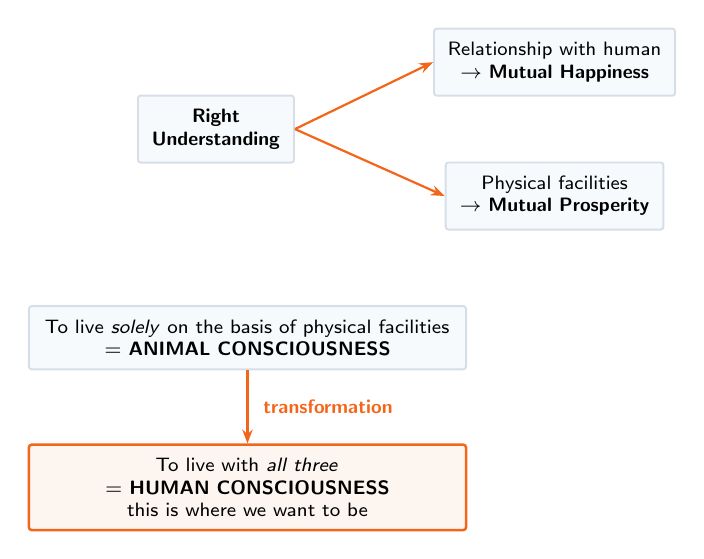
\begin{tikzpicture}[
  font=\sffamily\scriptsize,
  bx/.style={draw=rulegrey,fill=panel,rounded corners=1pt,line width=0.7pt,
             align=center,inner sep=5pt},
  hi/.style={draw=ocre,fill=tint,rounded corners=1pt,line width=0.9pt,
             align=center,inner sep=5pt},
  ar/.style={-{Stealth[length=5pt]},line width=0.8pt,draw=ocre}]

\node[bx] (ru) at (0,0) {\textbf{Right}\\\textbf{Understanding}};
\node[bx] (rel) at (4.3,0.85) {Relationship with human\\$\rightarrow$
  \textbf{Mutual Happiness}};
\node[bx] (pf) at (4.3,-0.85) {Physical facilities\\$\rightarrow$
  \textbf{Mutual Prosperity}};
\draw[ar] (ru.east) -- (rel.west);
\draw[ar] (ru.east) -- (pf.west);

\node[bx,text width=52mm] (ac) at (0.4,-2.65)
  {To live \emph{solely} on the basis of physical facilities\\
   $=$ \textbf{ANIMAL CONSCIOUSNESS}};
\node[hi,text width=52mm] (hc) at (0.4,-4.55)
  {To live with \emph{all three}\\
   $=$ \textbf{HUMAN CONSCIOUSNESS}\\
   {\scriptsize this is where we want to be}};
\draw[ar] (ac.south) -- node[right=2pt,font=\sffamily\scriptsize\bfseries,
  text=ocre]{transformation} (hc.north);
\end{tikzpicture}
\end{center}

Physical facilities: for humans --- \textbf{necessary but not complete}; for
animals --- \textbf{necessary and complete}.

From the diagram we can say: for animals, physical facilities are necessary as
well as complete, whereas for human beings they are necessary but not
complete. Working only for physical facilities is living with Animal
Consciousness. Working for right understanding as the first priority, followed
by relationship and physical facilities, implies living with Human
Consciousness.

\textbf{The transformation} from Animal Consciousness to Human Consciousness
can be accomplished only by working for \textbf{right understanding as the
first priority}. This transformation forms the basis for human values and
value-based living. The content of education is the understanding of harmony
at all four levels of our existence --- from myself to the entire existence;
and \emph{sanskar} (right living) refers to the ability to live in harmony at
all four levels. This dimension of society works to ensure `right
understanding' and `right feelings' in every individual, i.e. the
all-encompassing solution called \emph{samadhan}, and ensures that our
succeeding generations have both the content and the environment available to
work towards achieving their goal of continuous happiness and prosperity.

\section{E. Human Being as Co-existence of Self (`I') and Body (Chapter 5)}

% ------------------------------------------------------------------------ 23
\Q{23}{Distinguish between the needs of the Self and the needs of the
  Body.}{\tg{SEE}\mmk{5}}

\ans A human being is the \textbf{co-existence of the Self (`I') and the
Body}, with an exchange of information between the two. Their needs are
fundamentally different:

\renewcommand{\arraystretch}{1.3}
\arrayrulecolor{rulegrey}
\begin{longtable}{P{22mm} P{63mm} P{63mm}}
\rowcolor{slate}\hdr{} & \hdr{Self (`I')} & \hdr{Body} \\ \hline \endfirsthead
\rowcolor{slate}\hdr{} & \hdr{Self (`I')} & \hdr{Body} \\ \hline \endhead
\textbf{Needs are} & Trust, respect, happiness\ldots\ i.e.
  \textbf{Happiness (sukha)} &
  Food, clothing, shelter, instruments\ldots\ i.e. \textbf{Physical Facilities
  (suvidha)} \\ \hline
\textbf{In time} & \textbf{Continuous} --- I want to be happy and respected
  all the time, not even for a moment otherwise. &
  \textbf{Temporary} --- food, clothes, shelter are needed only periodically.
  Even breathing is not continuous; we inhale, then exhale. \\ \hline
\textbf{In quantity} & \textbf{Qualitative} (no quantity) --- we cannot speak
  of one kg of respect or two litres of affection. Either the feeling is there
  or it is not. &
  \textbf{Quantitative} (limited in quantity) --- four chapattis, one bicycle.
  Beyond the limit, consumption becomes \emph{necessary and tasteful}
  $\rightarrow$ \emph{unnecessary but tasty} $\rightarrow$ \emph{unnecessary
  and tasteless} $\rightarrow$ \emph{intolerable}. \\ \hline
\textbf{Fulfilled by} & \textbf{Right understanding and right feelings} &
  \textbf{Physico-chemical things} --- food, clothing, etc. \\ \hline
\textbf{Activities} & Desiring, thinking, etc. --- knowing, assuming,
  recognising, fulfilling &
  Breathing, heartbeat, etc. --- recognising, fulfilling \\ \hline
\textbf{Type} & \textbf{Conscious} (non-material) &
  \textbf{Physico-chemical} (material) \\ \hline
\end{longtable}

\textbf{The confusion today.} A common mistake is that we mix these two sets
of needs and assume that ``all we need is physical facilities (\emph{suvidha}),
and that will automatically ensure happiness (\emph{sukha})''. The reality is
that we need both, since one is the need of the Body and the other the need of
`I'. \textbf{One cannot replace the other}, and the programmes for the two are
also different. For example, sitting in an air-conditioned room on a
comfortable sofa with a person for whom you have a feeling of opposition ---
the body is well taken care of, but you are unhappy. Our gross
misunderstandings today are: \textbf{Body $=$ `I'; \ Facilities $=$ Happiness;
\ Clothes $=$ Respect.}

\section{F. Harmony in the Self --- and with the Body (Chapters 6 \& 7)}

% ------------------------------------------------------------------------ 24
\Q{24}{How can we ensure harmony in the Self (`I')?}{\tg{CIE 1}\mmk{4}}

\ans The activities of \textbf{imaging (desire)}, \textbf{analysing (thought)}
and \textbf{selecting\,/\,tasting (expectation)} are constantly taking place
in `I'; together they are called \textbf{imagination}. Today these are largely
set either by \textbf{pre-conditioning (manyata)} or by \textbf{sensations
from the body} --- i.e. from the outside --- and are not self-verified on the
basis of our natural acceptance. In this state we are \emph{partantra}
(enslaved), and our desires, thoughts and expectations are in conflict among
themselves and with our own natural acceptance. This is the cause of
unhappiness.

The way to ensure harmony in the Self is a \textbf{four-step process}:

\begin{apts}
\item Becoming aware that the human being is the \textbf{co-existence of `I'
      and the Body}.
\item Becoming aware that the \textbf{Body is only an instrument of `I'}; `I'
      is the seer, doer and enjoyer.
\item Becoming aware of the activities of \textbf{desire, thought and
      expectation}, and passing each of these through your \textbf{natural
      acceptance}.
\item Understanding the \textbf{harmony at all levels of our existence} by
      verifying the proposals at the level of natural acceptance. This leads
      to \textbf{realization and understanding}, which in turn become the
      basis for desire, thought and expectation --- and this leads to harmony
      in `I' in continuity.
\end{apts}

\textbf{The outcome:} desires, thoughts and expectations become definite and
have a clear flow, so there is no contradiction; we have clarity about
ourselves, our basic aspiration and the way to fulfil it; we understand all
the levels of our living and live accordingly; and we live in a state of
\emph{svatantrata} --- self-organised in our imagination, behaviour and work.
This results in continuous happiness and prosperity.

\begin{keybox}
Realization \& Understanding (1, 2) $\rightarrow$ Desire (3) $\rightarrow$
Thought (4) $\rightarrow$ Expectation (5) \ $=$ \ \emph{svatantra}
(self-organised)
\end{keybox}

% ------------------------------------------------------------------------ 25
\Q{25}{Define Sanyama and Svasthya. How are the two related?}{\mmk{4--5}}

\ans The harmony of `I' with the Body is in the form of \textbf{Sanyama} on
the part of `I' and \textbf{Svasthya} on the part of the Body.

\begin{abul}
\item \textbf{Sanyama (Self-regulation):} the feeling of responsibility in the
      Self (`I') for \textbf{nurturing, protecting and rightly utilising} the
      Body.
\item \textbf{Svasthya (Health):} the state of the Body when it is \textbf{fit
      to act according to the needs of the Self (`I')}, and there is
      \textbf{harmony among the different parts of the Body}.
\end{abul}

\textbf{Relation: Sanyama is the basis of Svasthya.} When I live with Sanyama,
there is harmony among the different parts of the Body and the Body is fit to
be used as an instrument of `I'. If there is Sanyama, health can be ensured;
if Sanyama is not there, even good health can be lost. Today, in place of
being responsible to the Body, we rely more on medication; we go for newer
sources of sensual pleasure and irresponsible practices in living, and thus
produce new diseases day by day. An increase in hospitals or medical grants is
no substitute for Sanyama.

% ------------------------------------------------------------------------ 26
\Q{26}{``Realization and understanding are essential for happiness and
  harmony.'' Explain.}{\tg{SEE}\mmk{5}}

\ans Happiness is being in a state of harmony; unhappiness is a state of
conflict and contradiction. We have seen that this conflict is primarily
\textbf{inside us} --- between our imagination (desire, thought, expectation)
and our natural acceptance.

As long as our desires are being set from the outside --- by a sensation from
the body or by a pre-conditioning (\emph{manyata}) --- there is every chance
that we are in conflict, and we are \emph{partantra} (enslaved). Not only are
the desires, thoughts and expectations in conflict among themselves, they are
also in conflict with our own natural acceptance, and this creates
unhappiness.

Through the process of self-exploration, the activities of \textbf{realization
and understanding} get activated. Once we start operating at the level of
realization and understanding, our desires, thoughts and expectations get
aligned with our own natural acceptance, and we become \emph{svatantra}
(self-organised). There is self-organisation in my activities, leading to
continuity of happiness --- this is \textbf{harmony in the Self (`I')}.

Further, since the understanding is invariant, the desires arising from it are
also definite, and hence the thoughts, selections, behaviour and work are also
in harmony. This is what gives \textbf{definiteness of human conduct}.
Realization and understanding are therefore not optional extras --- they are
the very basis of continuous happiness, which is the basic human aspiration.

% ---------------------------------------------------------------------------
%  UNIT II -- Chapters 8 and 9
% ---------------------------------------------------------------------------
\chapter{Unit II --- Harmony in the Family and in the Society: From Family
  Order to World Family Order}
\chaptermark{Unit II --- Chapters 8 and 9}

\section{A. Relationship, Justice and the State Today (Chapter 8)}

% ------------------------------------------------------------------------ 27
\Q{27}{``Family is a natural laboratory to understand human relationships''
  --- elaborate. \emph{(Also set as:} Relationship IS, and it exists between
  one jeevan and the other jeevan. Examine.\emph{)}}{\tg{CIE 2 QB}%
  \tg{CIE-II 2025}\mmk{5}}

\ans The family is the \textbf{basic unit of human interaction}. Each one of
us is naturally a part of a family that includes father, mother, brothers and
sisters, and then grandparents, aunts, uncles, cousins. These relationships
are a reality of our life --- we are \emph{born into} them; we have not
created them.

Here is the set of proposals the text asks us to verify:

\begin{apts}
\item \textbf{Relationship IS, and it exists between the Self (`I') and the
      other Self (`I').} It is not possible to create the relationships that
      are existent in a family; we are naturally born into them. It is the
      person's self which is primarily related to the other person's self. The
      Body is only a means to express or receive our relationship --- the Body
      is incapable of understanding as well as having feelings. For example, a
      mother feels related to the child she has given birth to; the body of
      the child has its source in the body of the mother, but neither body has
      feelings --- it is the Self of the mother and the child who feel
      connected.
\item \textbf{The Self (`I') has feelings in a relationship, and these
      feelings are between `I' and `I'.} Who wants trust in relationship ---
      you or the Body? The answer is, I want trust; and from the other `I'.
      There is no part of the body that wants trust or respect.
\item \textbf{These feelings in the Self are definite --- they can be
      identified with definiteness.} They are the values characterising
      relationships: trust, respect, affection, and so on.
\item \textbf{Recognising and fulfilling these feelings leads to mutual
      happiness in relationship.}
\end{apts}

\textbf{Why the family is a laboratory.} By living in relationships at all
times in the family, we get the occasion to gain the assurance that the other
person is an \textbf{aid to me and not a hindrance}. In the family we learn to
recognise relationship, recognise the definite feelings or values, and learn
how to fulfil them. The evaluation that takes place mutually in these close
relationships, leading to mutual happiness, instils a confidence in us that we
can live the right way with human beings. The family is thus a laboratory of
sorts in which we live our understanding. On getting assured, it becomes easy
to see that \textbf{society is an extension of family}, and that it is
possible to live in harmony with every human being --- thus laying the
foundation for an undivided human race, from \emph{family order} to
\emph{world family order}.

% ------------------------------------------------------------------------ 28
\Q{28}{What is `justice'? What are its four elements? Is it a continuous or a
  temporary need?}{\tg{SEE}\tg{CIE 2 QB}\tg{Scheme}\mmk{5}}

\ans \textbf{Justice is the recognition of values (the definite feelings) in
relationship, their fulfilment, and the right evaluation of the fulfilment
resulting in mutual happiness (Ubhay-tripti).} Justice concerns itself with
the proper ordering of things and people within a society.

\begin{keybox}
\textbf{The four elements of justice:}
\begin{enumerate}[label=\textbf{\color{ocre}\arabic*.},leftmargin=2.0em,
  itemsep=1pt,topsep=3pt,parsep=0pt]
\item \textbf{Recognition of values} --- recognising the definite feelings in
      the relationship
\item \textbf{Fulfilment} of those values
\item \textbf{Evaluation} of the fulfilment
\item \textbf{Mutual happiness} ensured
\end{enumerate}
\vspace{3pt}
When all four are ensured, justice is ensured. \textbf{Mutual fulfilment is
the hallmark of justice.}
\end{keybox}

\begin{center}\small\sffamily\color{slate}
Self (`I') ---relationship--- Self (`I') \ $\rightarrow$ \ Recognise the
VALUES \ $\rightarrow$ \ Fulfilment of VALUES \ $\rightarrow$ \ Evaluate the
fulfilment \ $\rightarrow$ \ Mutual happiness
\end{center}

\textbf{Is it continuous or temporary?} Justice is a \textbf{continuous need}.
Justice is essential in all relationships --- be it with the small kid in your
house, your old grandpa, the maid in the house, your fast friends or your
distant relations. We want justice not on a few occasions but \emph{every
moment}, and in every relationship, not just a few. We need to grow up in
relationships to ensure the continuity of justice in all our relationships. It
is also worth asking whether justice will get ensured in the family or in
courts of law --- in justice there is \emph{mutual fulfilment} for both
parties, which a judgement and punishment cannot deliver.

% ------------------------------------------------------------------------ 29
\Q{29}{What is the meaning of justice in human relationships? How does it
  follow from family to world family?}{\tg{CIE 2}\tg{SEE}\tg{Scheme}\mmk{5}}

\ans Justice is the recognition of values (the definite feelings in a
relationship), their fulfilment, and the right evaluation of the fulfilment
resulting in mutual happiness. There are four elements: recognition of values,
fulfilment, evaluation, and mutual happiness ensured. When all four are
ensured, justice is ensured; mutual fulfilment is the hallmark of justice.

\textbf{From family to world family.} Justice \textbf{starts from the family
and slowly expands to the world family}. The child gets an understanding of
justice in the family. With this understanding, he\,/\,she goes out into
society and interacts with people. All of us are children at some point of
time and grow into adults. In the family we learn to recognise relationship,
recognise the definite feelings or values, and learn how to fulfil them. The
evaluation that takes place mutually in close relationships, leading to mutual
happiness, instils a confidence in us that we can live the right way with
human beings; unless this confidence is ensured, we remain shaky in
relationships.

\textbf{If the understanding of justice is ensured in the family, there will
be justice in all the interactions we have in the world at large.} If we do
not understand the values in relationships, we are governed by our petty
prejudices and conditionings. We may treat people as high or low based on
their body (particular caste, or sex or race or tribe), on the basis of the
wealth one possesses, or the belief systems that one follows. All this is a
source of injustice and leads to a \emph{fragmented society}, while our
natural acceptance is for an \emph{undivided society and universal human
order}.

Having explored the harmony in human beings, we are able to explore the
harmony in the family. This enables us to understand the harmony at the level
of society and nature\,/\,existence. And this is the way the harmony in our
living grows --- we slowly get the competence to live in harmony with all
human beings.

% ------------------------------------------------------------------------ 30
\Q{30}{What is the outcome when we try to identify relationships based on the
  exchange of physical facilities?}{\mmk{5}}

\ans We are unable to see ourselves as the co-existence of the Self (`I') and
the Body. As a result we see ourselves as a body and the other as a body, and
we subsequently \textbf{reduce our relationships and the feelings in the
relationship to the level of the body}. We tend to assume that we have
relationship with our blood-related family members only.

As a result of this mistaken assumption, we have \textbf{reduced our
expectations in relationships to the mere fulfilment of physical facilities}.
We evaluate all our relationships in terms of material things like money,
property, etc. In short, the purpose of relationship has been reduced to
physical and material needs and their exchange. Hence we feel that working for
physical facilities alone is enough, or we assume that as long as we
accumulate physical facilities and provide the same to the other, the
relationship is automatically fulfilled.

\textbf{The outcome.} Suppose your father earns enough money and ensures that
your physical needs are taken care of, but does not spend time with you, does
not care for you, or instead behaves badly with you --- would you feel
satisfied? The answer is NO. Nowadays we also hear of youngsters earning a lot
of money who, instead of taking care of their parents and fulfilling their
needs of feelings at the level of `I' (trust, respect, affection), just put
their parents in some old-age home. The parents have plenty to eat, good
clothes, a big TV, servants --- but this is not fulfilling for them, since the
needs of the `I', the feelings in `I', have been totally ignored.

\textbf{The fact is:} what we need first is the \textbf{right understanding},
and this is not ensured by having money. Secondly, we need the \textbf{feelings
in relationships} to be fulfilled, which is also not ensured by having money.

\section{B. The Values in Human Relationships (Chapter 8)}

% ------------------------------------------------------------------------ 31
\Q{31}{Enumerate the important values which lie at the base of good
  relationships. \emph{(Also set as:} List the foundation value and the
  complete value in human relationship, and explain each with one
  example.\emph{)}}{\tg{CIE 2 QB}\mmk{5}}

\ans Being in relationship, we have feelings for the other. These feelings
cannot be replaced by any material or physical things. They are definite and
they are the values in a relationship. There are \textbf{nine} such values:

\renewcommand{\arraystretch}{1.3}
\arrayrulecolor{rulegrey}
\begin{longtable}{C{7mm} P{45mm} P{95mm}}
\rowcolor{slate}\hdr{\#} & \hdr{Value} & \hdr{Meaning (as defined in the text)}
  \\ \hline \endfirsthead
\rowcolor{slate}\hdr{\#} & \hdr{Value} & \hdr{Meaning (as defined in the text)}
  \\ \hline \endhead
\qn{1} & \textbf{Trust} (Vishvas) & To be assured that each human being
  inherently wants oneself and the other to be happy and prosperous.
  \textbf{The foundation value} (adhara mulya). \\ \hline
\qn{2} & \textbf{Respect} (Sammana) & Right evaluation --- to be evaluated as
  I am, without over-, under- or otherwise evaluation. \\ \hline
\qn{3} & \textbf{Affection} (Sneha) & The feeling of being related to the
  other; the acceptance of the other as one's relative. \\ \hline
\qn{4} & \textbf{Care} (Mamata) & The feeling to nurture and protect the body
  of our relative. \\ \hline
\qn{5} & \textbf{Guidance} (Vatsalya) & The feeling of ensuring right
  understanding and right feelings in the other (my relative). \\ \hline
\qn{6} & \textbf{Reverence} (Shraddha) & The feeling of acceptance of
  excellence in the other. \\ \hline
\qn{7} & \textbf{Glory} (Gaurava) & The feeling for someone who has made
  efforts for excellence. \\ \hline
\qn{8} & \textbf{Gratitude} (Kritagyata) & The feeling of acceptance for those
  who have made effort for my excellence. \\ \hline
\qn{9} & \textbf{Love} (Prema) & The feeling of being related to all.
  \textbf{The complete value} (purna mulya). \\ \hline
\end{longtable}

\textbf{Foundation value --- Trust}, with example: In a family, when a member
fails to do something for me, if I am assured that at the level of intention
he\,/\,she means well for me and only the competence was lacking, I do not get
hurt; I become a help to him\,/\,her. A relationship without trust results in
opposition; the relationship itself gets shaken up. Lack of trust is what
ultimately leads to extreme situations like war.

\textbf{Complete value --- Love}, with example: It starts with identifying
that I am related to one other human being (the feeling of affection) and
slowly expands to the feeling of being related to all human beings. When I am
able to feel related even to a stranger on the road --- recognising that at
the level of `I' he\,/\,she is exactly like me --- that is love. This feeling
of love lays down the basis of an \textbf{Undivided Society}.

Two useful points the text stresses: the basic values to be understood are
\textbf{trust and respect} --- if we have these, the remaining values flow
quite naturally. And \textbf{only Care (mamata) requires physical facilities};
for all the other feelings, what we essentially need is their proper
understanding.

% ------------------------------------------------------------------------ 32
\Q{32}{What do you understand by trust? Differentiate between intention and
  competence with examples. Why is this distinction important?}%
  {\tg{CIE 2}\tg{SEE}\tg{CIE-II 2025}\mmk{5}}

\ans \textbf{Trust (vishvas)} is defined as: ``\emph{To be assured that each
human being inherently wants oneself and the other to be happy and
prosperous.}'' We feel assured of the other person when we are sure that the
other wants to work for my happiness and prosperity. Whenever I feel the other
will deny my happiness and\,/\,or prosperity, I am afraid of that person.
Trust is the \textbf{foundation value} (adhara mulya) of relationship.

To understand it, examine four proposals: (1) I want to make myself happy;
(2) I want to make the other happy; (3) The other wants to be happy; (4) The
other wants to make me happy. Answering the fourth with deep exploration is
the basis of gaining trust in the other. On examining, we find there are
\textbf{two parts} in this exploration:

\begin{cmptable}{Intention (natural acceptance) --- \emph{wanting to}}%
                {Competence (ability to fulfil) --- \emph{being able to do}}
1a) I want to be happy \ \checkmark\newline
2a) I want to make the other happy \ \checkmark\newline
3a) The other wants to be happy \ \checkmark\newline
4a) The other wants to make me happy \ \checkmark \ (after exploration) &
1b) I am always happy \ ?\newline
2b) I always make the other happy \ ?\newline
3b) The other is always happy \ ?\newline
4b) The other always makes me happy \ ? \\ \hline
\textbf{What we really want to be} & \textbf{What we are} \\ \hline
\end{cmptable}

\textbf{The mistake we make.} When we judge ourselves, we judge on the basis
of our \emph{intention}; when we judge the other, we judge on the basis of
his\,/\,her \emph{competence}. We say ``I wanted to do well, but I could
not'' --- but for the other we say ``He did not want to do well''. ``Wanting
to'' is the intention; ``could not'' is the lack of competence.

\textbf{Example.} You are walking on your college campus and your close friend
walks by from the other direction. You look at him and smile, but he barely
notices you and keeps walking with his head down. You feel angry and
disappointed, and assume he wants to ignore you. Later you find out that he
was disturbed since he had lost his wallet. You immediately feel alright and
are not angry any more. What happened? You \textbf{doubted your friend's
intention}. It was not that he intended to ignore you; only that he was
preoccupied. Once you knew this, you realised it was not his intention but
only \textbf{his competence that was lacking} at that moment.

\textbf{Why the distinction is important.} Intention is \textbf{always
correct} and is the same in all of us; it is only the competence that is
lacking, which can be improved by right understanding. When we are assured of
the intention of the other and find that the competence is lacking, we
\textbf{become a help} to the other. When we doubt the intention of the other,
we \textbf{get into opposition}. You cannot have a problem in relationship
unless you have ended up doubting the intention of the other person, no matter
how close you are to them.

% ------------------------------------------------------------------------ 33
\Q{33}{In our behaviour, we generally observe our intention and others' lack
  of competence. Does it lead to mutual happiness? What is the alternative?
  Explain with an example.}{\tg{CIE 2 QB}\tg{Scheme}\mmk{5}}

\ans \textbf{No, it does not lead to mutual happiness.} We trust our own
intention while we are not ready to trust the other's intention. It is the
same for the others as well --- while the other trusts his\,/\,her own
intentions, he\,/\,she does not trust mine. Hence \textbf{mistrust is born and
we deny the relationship}.

When we are judging ourselves we are judging on the basis of our intention,
whereas when we are judging the other we are judging him on the basis of his
competence. We are sure that we want to make the other happy, but we are not
sure that the other wants to make us happy. We find that while we look at our
intention we are sure of it; we are not sure of the other's intention. We are
actually seeing their competence and making a conclusion on their intention
--- we say ``I wanted to do well, but I could not'', but for the other we say
``He did not want to do well''.

\textbf{The alternative.} We can see that we are not able to fulfil our
intentions in terms of our competence at all times; it is the same for the
other as well. We want to be related to the other, and we want the other to be
related to us, irrespective of who this other is. If we have trust in the
other, we are able to see the other as a \textbf{relative and not as an
adversary}. We then become ready to \textbf{become a help to the other}.
Intentions are always correct; it is only the competence that is lacking,
which can be improved by the right understanding.

\textbf{Example.} Suppose a friend promises to bring your notes to class and
forgets. If I doubt his intention (``he did not want to help me''), I get
irritated, we argue, and both of us are unhappy --- there is no mutual
happiness. If instead I am assured of his intention and see that only his
competence (memory, planning) was lacking, I do not get hurt; I remind him and
help him organise better next time. He is comfortable and so am I --- this is
mutual happiness, and his competence also improves.

% ------------------------------------------------------------------------ 34
\Q{34}{There is a common saying: ``If you trust everybody, people will take
  undue advantage of you.'' What is the basic error in this statement?
  \emph{(Also set as:} How can I trust a stranger?\emph{)}}%
  {\tg{CIE 2 QB}\tg{Scheme}\mmk{5}}

\ans \textbf{The basic error is that if we trust everybody, people will
\emph{not} take undue advantage of us.} On the contrary, it gives us
\textbf{inner strength} and we become far more effective in interacting with
and dealing with different people. This is simply because we already are
sitting with the knowledge of what the person truly wants, truly intends, even
though the person may not know this himself\,/\,herself.

Hence our ability to interact with people becomes far more effective, and in
the process \textbf{we don't get hurt, we don't get disturbed, and we end up
becoming an aid to the other}. In other words, becoming aware, having the
right understanding, and living with the assurance in the relationship does
not mean becoming ``stupid'' --- it only makes us \textbf{more competent}.
People can take advantage of you only if you \emph{do not} have the right
understanding, which is the state we are in today.

Further, what is being said is that we have \textbf{trust in the intention} of
everyone; but when it comes to \textbf{making a programme} with someone, I
evaluate my competence, I evaluate his competence, and make the programme
accordingly. This makes me more effective than if I did it otherwise, i.e. by
doubting his intention.

\textbf{``How can I trust a stranger?''} If you are able to see the
relationship with the person at the level of `I', you will see that the other
person is also like you. He\,/\,she too has natural acceptance for the same
things as you, wants to make himself\,/\,herself happy, and wants to make you
happy at the level of intention --- just as you do. But he\,/\,she may be
unaware of this fact, just as you were, and hence may be interacting with you
on the basis of your competence. \textbf{If we interact with or evaluate the
other person at the level of competence only, then there cannot be continuity
of trust.} In that case we end up doubting the other person, which causes a
sense of opposition in us; and since opposition is not naturally acceptable,
it creates a contradiction in us. Hence the way out is to relate to the other
person, to be able to see that at the level of natural acceptance we are the
same. We can then interact with the person based on their competence, and also
help them improve their competence.

\begin{keybox}
So, you can trust anyone \emph{for the intention part}. But don't assume that
his\,/\,her desires, thoughts and expectations are going to be right ---
he\,/\,she may lack competence. \textbf{The competence is to be evaluated
before you make a programme with the other.}
\end{keybox}

% ------------------------------------------------------------------------ 35
\Q{35}{What is the meaning of respect? What is the basis of respect for a
  human being? Do you see that the other human being is also similar to
  you?}{\tg{CIE 2 QB}\tg{SEE 2025}\mmk{5}}

\ans \textbf{Respect (sammana) means ``Right Evaluation''} --- to be evaluated
as I am. Usually, however, we make mistakes in evaluation in three ways:

\renewcommand{\arraystretch}{1.3}
\arrayrulecolor{rulegrey}
\begin{longtable}{P{45mm} P{40mm} P{62mm}}
\rowcolor{slate}\hdr{Mistake} & \hdr{Meaning} & \hdr{Example} \\ \hline
\endfirsthead
\rowcolor{slate}\hdr{Mistake} & \hdr{Meaning} & \hdr{Example} \\ \hline
\endhead
\textbf{Over evaluation} (adhi-mulyana) & To evaluate more than what it is &
  Your father tells guests, ``My son is the greatest scholar in India!'' ---
  you feel uncomfortable when wrongly flattered. \\ \hline
\textbf{Under evaluation} (ava-mulyana) & To evaluate less than what it is &
  ``My son is a good for nothing; he must be the laziest person in all of
  India!'' --- you feel uncomfortable when condemned. \\ \hline
\textbf{Otherwise evaluation} (a-mulyana) & To evaluate otherwise than what it
  is & ``You donkey! Can't you even understand this much?'' --- you are
  evaluated as something else, since you are a human being and not something
  else. \\ \hline
\end{longtable}

Any kind of over, under or otherwise evaluation makes us uncomfortable; we
feel `disrespected'. \textbf{We say we have been disrespected when we are
wrongly evaluated.}

\textbf{The basis for respect.} A human being is a co-existence of Self (`I')
and Body. Right evaluation is on the basis of the acceptance of this
co-existence. If we respect a human being on the basis of `I', the following
are true for every human being:

\begin{apts}
\item I want continuous happiness and prosperity --- \emph{the other too wants
      to be continuously happy and prosperous}.
\item To be happy, I need to understand and live in harmony at all four levels
      of my living --- \emph{the other also needs to understand and live in
      harmony at all four levels of his\,/\,her living}.
\item The activities in me (`I') are continuous --- we can check this for
      desire, thought and expectation --- \emph{it is the same for the other
      `I' as well}.
\end{apts}

Based on these three evaluations we conclude:

\begin{abul}
\item Our \textbf{basic aspiration} is the same --- we both want continuous
      happiness and prosperity.
\item Our \textbf{programme of action} is the same --- to understand and live
      in harmony at all four levels of our living.
\item Our \textbf{potential} is the same --- the activities and powers of the
      self are continuous and the same in both of us at the level of `I'.
\end{abul}

\begin{keybox}
$\Rightarrow$ \ \textbf{The other is similar to me.}
\end{keybox}

Yes --- when we are able to see that the other is similar to me, we are able
to recognise the feeling of respect in the relationship. If not, we either
hold ourselves more or less than the other, and this only leads to
differentiation. The difference between me and the other can only be at the
level of \emph{understanding} (not information), and this manifests as a
meaningful responsibility, not as a criterion for superiority or inferiority:
if the other has better understanding than me, I want to understand from the
other; if the other has less understanding than me, I accept the
responsibility to improve the understanding of the other.

% ------------------------------------------------------------------------ 36
\Q{36}{How do we differentiate in relationships on the basis of body, physical
  facilities or beliefs? What problems do we face because of such
  differentiation? \emph{(Also set as:} ``Discrimination leads to acrimony in
  relationships.'' Explain.\emph{)}}%
  {\tg{CIE 2}\tg{SEE}\tg{CIE-II 2025}\tg{Scheme}\mmk{5}}

\ans Instead of respect being a basis of similarity or of \emph{right
evaluation}, we have made it into something on the basis of which we
differentiate. We differentiate on three bases:

\renewcommand{\arraystretch}{1.3}
\arrayrulecolor{rulegrey}
\begin{longtable}{P{22mm} P{60mm} P{65mm}}
\rowcolor{slate}\hdr{Basis} & \hdr{How we differentiate} &
  \hdr{Problems created (as per the scheme)} \\ \hline \endfirsthead
\rowcolor{slate}\hdr{Basis} & \hdr{How we differentiate} &
  \hdr{Problems created (as per the scheme)} \\ \hline \endhead
\textbf{Body} & \textbf{Sex\,/\,Gender} --- respect males more than females
  (or the reverse), ignoring that being male or female is an attribute of the
  body, not of `I'. &
  Issue of women's rights; women protesting and demanding equality in
  education, in jobs and in people's representation. People are insecure and
  afraid of one another based on their gender. \\ \hline
 & \textbf{Race} --- skin colour, Mongolian\,/\,Aryan\,/\,Dravidian race, or
  caste taken as high and low. &
  Many movements and protests against racial discrimination and demands for
  equality; racial attacks; movements against caste discrimination; people
  living in fear of racism, racist attacks, casteism and discrimination.
  \\ \hline
 & \textbf{Age} --- notions such as ``one must respect elders''; age relates
  to the body, not to `I'. &
  Protests and movements demanding equal rights for children on the one hand
  and rights for elderly people on the other; the \emph{generation gap}, a
  source of tension in many families. \\ \hline
 & \textbf{Physical strength} --- treating the stronger person differently. We
  think we are respecting, while it is actually fear. &
  Many programmes, awards and titles based on physical strength, which have
  nothing to do with how the person is at the level of `I'. \\ \hline
\textbf{Physical facilities} & \textbf{Wealth} --- the ``rich person'' gets
  idolised; we never check whether such people feel prosperous or are happy. &
  Class struggle and movements to do away with class-differentiation; many
  people suffering from a lack of self-esteem, and some even committing
  suicide. \\ \hline
 & \textbf{Post} --- respect on the basis of a person's position; the post
  wrongly evaluated as the mark of excellence. &
  Protests against high-handed government officials. At the level of the
  individual, it leads to depression, since those who do not qualify for a
  post feel they will not get respect in society. \\ \hline
\textbf{Beliefs} & \textbf{`Isms'} --- capitalism, socialism, communism, etc.;
  belief systems adopted since childhood. &
  Fights, turmoil, terrorism and war; people converting from one `ism' to
  another in order to get more respect. \\ \hline
 & \textbf{Sects} --- a set of beliefs reflected in traditions and practices;
  only those with a similar belief system are considered `own' and worthy of
  respect. &
  Countless religions and sects, each with its own movement to ensure there is
  no discrimination against people of their belief; demands for special
  provisions in jobs and in education; clashes that even turn violent.
  \\ \hline
\end{longtable}

\textbf{The way out.} To move beyond differentiation we have to understand the
human being as the co-existence of Self (`I') and Body, and then base our
evaluation on the Self (`I'), where we find we are similar to the other in
natural acceptance, programme of action and potential. This becomes the basis
of the feeling of respect. We differ from the other only in terms of
competence, and there we either learn from the other or take the
responsibility of helping the other improve.

% ------------------------------------------------------------------------ 37
\Q{37}{What is the difference between respect and disrespect? Which of the two
  is naturally acceptable to you? \emph{(Also set as:} List the differences
  between respect and differentiation.\emph{)}}{\tg{CIE 2}\tg{CIE 2 QB}%
  \tg{SEE}\mmk{5}}

\ans
\begin{cmptable}{Respect (Right Evaluation)}{Disrespect \,/\, Differentiation}
Means \textbf{right evaluation} --- to evaluate the other as he\,/\,she is. &
Means \textbf{wrong evaluation} --- over evaluation, under evaluation, or
  otherwise evaluation. \\ \hline
Evaluation is done at the level of the \textbf{Self (`I')}. &
Evaluation is done at the level of the \textbf{Body, physical facilities or
  beliefs}. \\ \hline
Based on \textbf{similarity} --- the other is similar to me in aspiration,
  programme of action and potential. &
Based on \textbf{difference} --- sex, race, age, physical strength, wealth,
  post, `isms', sects. \\ \hline
Leads to a feeling of relationship, mutual fulfilment and ease in both. &
Leads to a feeling of opposition, discomfort, and problems in relationship.
  \\ \hline
It is \textbf{continuous} --- once we have this feeling out of understanding,
  it remains there all the time; it is the state of harmony between one human
  and the other. &
It is \textbf{unstable} and changes with the person's body, possessions or
  position, and hence needs constant re-establishment. \\ \hline
Does not require the other to do anything special; the fact that you are human
  is enough for me to respect you. &
Makes everyone run around trying to become ``special'' to earn respect ---
  which fetches only attention, not respect. \\ \hline
Its outcome is an \textbf{undivided society}. &
Its outcome is a \textbf{fragmented society}. \\ \hline
\end{cmptable}

\textbf{Which is naturally acceptable? Respect.} Verify it for yourself: what
is naturally acceptable to you --- the feeling of respect or disrespect for
yourself? And for the other? You will find that each one of us has an
acceptance for the feeling of respect. Just as we desire this, the other also
expects the same. \textbf{Every human being wants to respect and be
respected.} No human being finds disrespect acceptable in relationship.

% ------------------------------------------------------------------------ 38
\Q{38}{Define affection. How does affection lead to harmony in the family?
  What is the role of physical facilities in the fulfilment of this
  feeling?}{\tg{CIE 2}\mmk{5}}

\ans \textbf{Affection (sneha) is the feeling of being related to the other.}
Affection comes when I recognise that we both want to make each other happy
and that both of us are similar. Then, for the first time, I feel that I am
related to the other, that the other is a relative of mine. ``\emph{This
feeling of acceptance of the other as one's relative is the feeling of
affection or sneha in relationship.}''

\textbf{How it leads to harmony in the family.}

\begin{abul}
\item This feeling comes only if \textbf{Trust and Respect are already
      ensured}. Without trust and respect you feel the other is trying to make
      you unhappy and does not wish well for you, and hence you can never feel
      affection for him\,/\,her; you always see the other as being in
      opposition. That is why in families people live together for years and
      still don't feel related to each other --- the basic trust and respect
      are missing.
\item When affection is there, I have come to realise that I am related to you
      and you are related to me. There is no doubt on intention, hence no
      irritation, anger or feeling of opposition --- and therefore no fights.
      This is harmony in the family.
\item Affection also \textbf{removes competition}. Competition results when
      there is a lack of affection. When there is affection, I \emph{help the
      other grow}; when I miss this feeling, I try to beat the other and act
      as an opponent. What is naturally acceptable to us is excellence, not
      competition --- and we humans can grow only in relationships.
\item Affection is the starting point of the expansion outward: it starts with
      being related to one, and slowly expands to the feeling of being related
      to everyone, which is \textbf{love} --- and this lays the basis of an
      undivided society.
\end{abul}

\textbf{Role of physical facilities.} Affection is a feeling in `I'; it is
\emph{not} fulfilled by physical facilities. Of the nine values, \textbf{only
Care (mamata) requires physical facilities}, because care is the feeling to
nurture and protect the body of our relative. For affection and the other
feelings, what we need essentially is their \emph{proper understanding}.
Trying to express affection only by giving things is precisely the mistake of
reducing relationship to the exchange of physical facilities.

% ------------------------------------------------------------------------ 39
\Q{39}{Explain the feelings of care, guidance, reverence, glory and gratitude.
  \emph{(Also set as:} Illustrate the natural acceptance values in
  relationship with an example for each --- (i) Reverence (ii)
  Glory.\emph{)}}{\tg{CIE-II 2025}\mmk{5}}

\ans
\begin{abul}
\item \textbf{Care (Mamata)} --- the feeling to \textbf{nurture and protect
      the body of our relative}. We understand a human being as a co-existence
      of the Self (`I') and the Body, and the Body is an instrument of `I'.
      Based on this understanding, we take the responsibility of nurturing and
      protecting the body of our relative. \emph{(This is the only value that
      requires physical facilities.)}
\item \textbf{Guidance (Vatsalya)} --- the feeling of \textbf{ensuring right
      understanding and right feelings in the other} (my relative). We
      understand the need of our Self for right understanding and feelings; we
      also understand that the other is similar to me in the faculty of
      natural acceptance, in the desire for continuous happiness, and in the
      potential of desire, thought and expectation. Right understanding is
      also a need of the other, and the other is related to me; hence I have
      the responsibility to help the other.
\item \textbf{Reverence (Shraddha)} --- the feeling of \textbf{acceptance of
      excellence in the other}. We aspire for continuous happiness, and to
      realise it we must understand harmony at all levels of living and live
      accordingly. When we see that the other has achieved this excellence, we
      have a feeling of reverence for him\,/\,her. \emph{Example:} a teacher
      who has actually understood harmony at all four levels and lives
      accordingly --- I accept that excellence in them, and that acceptance is
      reverence.
\item \textbf{Glory (Gaurava)} --- the feeling for someone who has \textbf{made
      efforts for excellence}. There have been people in history, or even
      around us, who invest their time, energy and belongings to achieve
      excellence and to make others excellent. This gives us a feeling of
      glory for them. \emph{Example:} a person who gave up a comfortable
      career to work for the right understanding of others --- I accept their
      \emph{effort} towards excellence, and that acceptance is glory.
\item \textbf{Gratitude (Kritagyata)} --- the feeling of \textbf{acceptance
      for those who have made effort for my excellence}. Today, what we
      generally call gratitude is a feeling coming out of assistance at the
      level of physical facilities; this feeling is short-lived, since the
      physical facility and the sensation from it are also short-lived. But
      gratitude coming out of someone doing something for my \emph{right
      understanding is permanent}, since the happiness we get from right
      understanding is permanent.
\end{abul}

\begin{keybox}
\textbf{\sffamily Reverence, glory and gratitude --- the distinction that is
examined.} Reverence is for the \emph{excellence achieved}; glory is for the
\emph{effort made} towards excellence; gratitude is for the effort made
towards \emph{my} excellence. The object shifts: their achievement, their
effort, their effort for me.
\end{keybox}

% ------------------------------------------------------------------------ 40
\Q{40}{Define love. How can you say that love is the complete value?
  \emph{(Also set as:} ``The feeling of love lays down the basis of an
  undivided society.'' Explain.\emph{)}}{\tg{SEE}\tg{CIE 2 QB}\mmk{5}}

\ans \textbf{The feeling of being related to all is love (prema).}

\textbf{Why it is the complete value.} This feeling or value is also called
the \textbf{complete value (Purna mulya)}, since it is the feeling of
relatedness to all human beings. The other values are directed towards one
other person --- affection is the feeling of being related to \emph{the
other}, care is towards \emph{my relative's} body, guidance towards \emph{my
relative}. Love is the same feeling extended to everyone, \textbf{without
exception}. Hence nothing more remains to be added; it completes the set of
values in relationship. It starts with identifying that one is related to
\emph{the other} human being (the feeling of affection) and it slowly expands
to the feeling of being related to \emph{all} human beings.

\begin{center}\small\sffamily\color{slate}
Trust \ $\rightarrow$ \ being related to one (Affection) \ $\rightarrow$ \
being related to everyone (Love)
\end{center}

\textbf{How it lays the basis of an undivided society.} The feeling of love
leads to an \textbf{Undivided Society (Akhanda Samaja)} --- it starts from the
family and slowly expands to the world family. Every human being has a natural
acceptance for relatedness up to the world family in the form of love. The
feeling of being related to every human being leads to our participation in an
undivided society. With the understanding of values in human relationships, we
are able to recognise the connectedness with every individual correctly, and
fulfil it. Conversely, if we do not understand the values in relationship, we
are governed by our petty prejudices and conditionings; we treat people as
high or low on the basis of body, wealth or belief. All this is a source of
injustice and leads to a fragmented society, while our natural acceptance is
for an undivided society and universal human order. Love is precisely the
feeling that removes every basis for such fragmentation, and hence it is the
foundation of the undivided society.

\section{C. Harmony in the Society (Chapter 9)}

% ------------------------------------------------------------------------ 41
\Q{41}{What is the comprehensive human goal? Explain how this is conducive to
  sustainable happiness and prosperity for all. How can these four goals
  create harmony in society?}{\tg{CIE 2}\tg{CIE 2 QB}\tg{SEE 2025}\mmk{5--6}}

\ans In order to facilitate the fulfilment of the basic aspirations of all
human beings in society, the following \textbf{comprehensive human goal} needs
to be understood:

\renewcommand{\arraystretch}{1.3}
\arrayrulecolor{rulegrey}
\begin{longtable}{C{7mm} P{45mm} P{26mm} P{62mm}}
\rowcolor{slate}\hdr{\#} & \hdr{Goal} & \hdr{Level} & \hdr{Meaning} \\ \hline
\endfirsthead
\rowcolor{slate}\hdr{\#} & \hdr{Goal} & \hdr{Level} & \hdr{Meaning} \\ \hline
\endhead
\qn{1} & \textbf{Right Understanding} (Samadhana) & In every individual &
  Right understanding is necessary for all human beings. When one does not
  have it, one remains disturbed and also acts so as to create disharmony with
  other human beings and with the rest of nature. \\ \hline
\qn{2} & \textbf{Prosperity} (Samriddhi) & In every family &
  The family is able to identify its needs and is able to
  produce\,/\,achieve more than its requirements. \\ \hline
\qn{3} & \textbf{Fearlessness (Trust)} (Abhaya) & In society &
  Every member of society feels related to everyone else, and therefore there
  is trust and fearlessness. \\ \hline
\qn{4} & \textbf{Co-existence} (Saha-astitva) & In nature &
  There is a relationship and complementarity among all the entities in
  nature, including human beings. \\ \hline
\end{longtable}

\textbf{How the four are related (and hence create harmony):}

\begin{apts}
\item The harmony in society \textbf{begins from the individual}. We need to
      ensure right understanding in the individual as the foundation of
      harmony in society.
\item With right understanding, the \textbf{need for physical facilities in
      the family can be ascertained}. By assessing our needs correctly and by
      producing more than required, the family can be prosperous.
\item Assurance of right understanding in the individuals and prosperity in
      the families, together with the understanding of human relationships,
      leads to harmony and \textbf{trust (fearlessness) in society}. When
      every individual is able to live harmoniously in relationship, and the
      needs of all the families are ensured, fearlessness (mutual trust) in
      society will naturally follow.
\item When human beings with right understanding interact with nature, it will
      be in consonance with \textbf{co-existence} and will be mutually
      enriching.
\end{apts}

\begin{keybox}
\textbf{1. Right Understanding \ $\rightarrow$ \ 2. Prosperity \ $\rightarrow$
\ 3. Fearlessness (trust) \ $\rightarrow$ \ 4. Co-existence}
\end{keybox}

\textbf{Why it is conducive to sustainable happiness and prosperity for all.}
With little exploration, we find that \textbf{all four are required}; we are
not satisfied with anything less. This is the basic minimum requirement to
ensure sustainable happiness and prosperity, and also the maximum we can think
of --- we cannot cut down any of them, and the moment we leave any one out,
there will be a loss of continuity and the goal cannot be achieved. The goal
is not only comprehensive but also \emph{universal}, i.e. equally applicable to
all human beings and for all times. Because it secures right understanding in
the individual (so happiness does not depend on sensation), prosperity in the
family (so the need is limited and met), fearlessness in society (so no one
lives in the fear of another), and co-existence with nature (so production
does not destroy its own base), the happiness and prosperity so achieved are
\textbf{sustainable} rather than temporary.

% ------------------------------------------------------------------------ 42
\Q{42}{Explain the comprehensive human goal. How does fearlessness follow from
  right understanding and prosperity?}{\tg{CIE 2}\mmk{5}}

\ans The four constituents of the comprehensive human goal are as listed in
\textbf{Q41}: right understanding in every individual, prosperity in every
family, fearlessness (trust) in society, and co-existence in nature.

\textbf{How fearlessness follows.} Fearlessness (\emph{abhaya}) in society
means that every member of society feels related to everyone else, and
therefore there is trust and fearlessness. It follows from the first two goals
in this sequence:

\begin{abul}
\item \textbf{From right understanding:} With right understanding, the
      individual is able to recognise that relationship \emph{is} --- that it
      exists at the level of `I' --- and is able to recognise and fulfil the
      values in that relationship (trust, respect, affection\ldots). Since
      trust means being assured that the other inherently wants my happiness
      and prosperity, an individual with right understanding \textbf{does not
      doubt the intention of the other}, and hence has no reason to fear the
      other. When every individual is able to live harmoniously in
      relationship, mutual trust in society naturally follows.
\item \textbf{From prosperity:} With right understanding, the need for
      physical facilities in the family can be ascertained; by assessing needs
      correctly and producing more than required, the family becomes
      prosperous. A family that feels prosperous has \textbf{no motive to
      exploit, hoard or grab} from another family --- on the contrary, the
      feeling of prosperity leads to sharing and becoming an aid to the other.
      Deprivation, by contrast, leads to exploiting the other. Hence when the
      needs of all the families are ensured, the basis of mutual fear between
      them disappears.
\end{abul}

Thus fearlessness is not something to be manufactured separately; it is the
\textbf{natural consequence} of right understanding in individuals plus
prosperity in families. This is why the text states the relation as the
sequence: \textbf{Right Understanding $\rightarrow$ Prosperity $\rightarrow$
Fearlessness (trust) $\rightarrow$ Co-existence.}

Contrast this with our state today: in place of working for fearlessness, we
are working for \emph{strategic powers}. In the name of defence we are
misusing the valuable resources of nature to make weapons and ammunition. We
are becoming increasingly more fearful of each other, paranoid that the other
human being is out to get me --- so most countries are busy preparing for war,
in the hope that more and more competence for war will lead to peace.

% ------------------------------------------------------------------------ 43
\Q{43}{Critically examine the state of society today in terms of the
  fulfilment of the comprehensive human goal.}{\tg{CIE 2 QB}\tg{SEE 2025}%
  \mmk{5--6}}

\ans
\renewcommand{\arraystretch}{1.3}
\arrayrulecolor{rulegrey}
\begin{longtable}{P{40mm} P{112mm}}
\rowcolor{slate}\hdr{Goal} & \hdr{Where we are today} \\ \hline \endfirsthead
\rowcolor{slate}\hdr{Goal} & \hdr{Where we are today} \\ \hline \endhead
\textbf{Right understanding in individuals} &
  We are not really working for this. We are talking so much about
  \emph{information and skills}, but ignoring the need for right
  understanding, ignoring the need to understand happiness correctly, and
  ignoring the need to understand and be in relationship. The programme to
  ensure the very first step is missing --- and the route to prosperity and
  social harmony is through right understanding only. \\ \hline
\textbf{Prosperity in families} &
  We are not able to see that the need for physical facilities is limited and
  that we can have more than what we need. We are only talking about how to
  \emph{generate more wealth}. Our economy, education and market lure
  individuals to generate as much wealth as possible. We feel proud declaring
  the number of billionaires and trillionaires, without ever evaluating
  whether this is taking us to the state of prosperity. \\ \hline
\textbf{Fearlessness (trust) in society} &
  In place of working for fearlessness, we are working for \emph{strategic
  powers}. In the name of defence we misuse the valuable resources of nature
  to make weapons and ammunition. We are becoming increasingly fearful of each
  other; most countries are busy preparing for war in the hope that more
  competence for war will lead to peace. We have organisations like the United
  Nations, but even there we do not have programmes to ensure mutual trust
  among people. \\ \hline
\textbf{Co-existence with nature} &
  Instead of co-existing, we are busy figuring out better ways to exploit
  nature. We have assumed that the goal of technological development is to get
  victory over nature, to subjugate the entities in nature and to disrupt
  nature's cycles. We have disregarded the obvious truth that nature is our
  basic support system, and that disturbing its balance will result in our own
  destruction. \\ \hline
\end{longtable}

\textbf{Conclusion.} We have missed out on the core things. There is a need to
re-align our focus towards ensuring right understanding and relationship. For
this we have to understand the harmony at all levels of our living, and move
from \emph{living with assumptions} to \emph{living with right
understanding}. Each one of us needs to start this journey within, to be able
to contribute towards the rectification of this dangerous situation.

% ------------------------------------------------------------------------ 44
\Q{44}{What are the five dimensions of human endeavour in society conducive to
  manaviya vyavastha? How are they helpful in achieving the comprehensive
  human goal?}{\tg{CIE 2 QB}\mmk{5}}

\ans These five dimensions broadly cover all the activities that are necessary
and fundamental to the harmonious existence of human society:

\begin{apts}
\item \textbf{Education -- Right Living (Siksha-Sanskara).} Education $=$ to
      understand harmony at all four levels of living. Right Living
      (\emph{sanskara}) $=$ the commitment and preparedness to live in harmony
      at all four levels of living. This dimension ensures `right
      understanding' and `right feelings' in every individual.
\item \textbf{Health -- Self-regulation (Svasthya-Sanyama).} \emph{Sanyama} is
      the feeling of responsibility for nurturing, protecting and rightly
      utilising the body; \emph{Svasthya} is the state of the body when it is
      fit to act according to the needs of the Self and there is harmony among
      the parts of the body. Sanyama is the basis of Svasthya.
\item \textbf{Justice -- Preservation (Nyaya-Suraksha).} Justice refers to
      harmony in the relationship \emph{between human beings} --- its
      recognition, fulfilment and evaluation leading to mutual happiness.
      Preservation refers to harmony in the relationship \emph{between the
      human being and the rest of nature}, leading to mutual prosperity ---
      i.e. \textbf{Enrichment (samvardhana), Protection (sanrakshana)} and
      \textbf{Right Utilization (sadupayoga)} of nature.
\item \textbf{Production -- Work (Utpadana-Karya).} Work is the labour that
      the human does on the rest of nature; Production is the physical
      facility obtained out of work. Two questions matter: \emph{what to
      produce?} (physical facilities for nurturing, protecting and rightly
      utilising the body) and \emph{how to produce?} (through a
      \textbf{cyclic (avartansheel) process}, in harmony with nature, ensuring
      that every unit is enriched).
\item \textbf{Exchange -- Storage (Vinimaya-Kosha).} Exchange is the
      exchanging of produce between members of society \emph{for mutual
      fulfilment, not for the madness of profit}; Storage is the storing of
      produce after the fulfilment of needs, \emph{with a view to right
      utilisation in the future, not hoarding}.
\end{apts}

\textbf{How they achieve the comprehensive human goal:}

\begin{cmptable}{Dimension}{Leads to}
Education -- Right Living (Siksha-Sanskara) &
  \textbf{Right understanding} (samadhana) in the individual \\ \hline
Health -- Self-regulation (Svasthya-Sanyama) &
  \textbf{Prosperity} (samriddhi) --- well-being of the body and
  identification of the need for physical facilities \\ \hline
Justice -- Preservation (Nyaya-Suraksha) &
  \textbf{Fearlessness} (abhaya) and \textbf{Co-existence} (saha-astitva)
  respectively \\ \hline
Production -- Work (Utpadana-Karya) &
  \textbf{Prosperity} and \textbf{Co-existence} --- production is done in
  harmony with nature \\ \hline
Exchange -- Storage (Vinimaya-Kosha) &
  \textbf{Prosperity} and \textbf{Fearlessness} --- when we store and exchange
  for mutual fulfilment and not for exploitation \\ \hline
\end{cmptable}

% ------------------------------------------------------------------------ 45
\Q{45}{Explain how production activities can be enriching to all the orders of
  nature. Give any two examples. \emph{(Also set as:} What is the avartansheel
  process of production?\emph{)}}{\tg{CIE 2 QB}\mmk{5}}

\ans On understanding the harmony at all levels of our living, it becomes
evident that there is an inherent balance in nature. So it is only natural
that any production system we design is \textbf{within the framework present
in nature}. When we look at the way nature is organised, two things become
apparent:

\begin{apts}
\item The systems in nature are \textbf{cyclic}, i.e. they are not open-ended.
\item The systems in nature are \textbf{mutually fulfilling or mutually
      enriching}.
\end{apts}

Thus the way to produce is through a \textbf{cyclical (avartansheel) process,
in harmony with nature}: (a) it has to be cyclic, and (b) it has to ensure
that every unit is enriched.

\textbf{Example 1 --- The seed and the soil (nature's own cycle).} When a seed
is planted in soil and water is added, it grows into a tree and in turn bears
leaves, flowers and fruits. The fruits ripen, leaves mature and fall to the
ground and enrich the soil, forming manure by decaying. Seeds are scattered
from the fruit into the soil and once again form a plant and bear fruit. This
way the soil gets enriched, seeds are multiplied and the tree grows ---
everything is regenerated. The process is both cyclic and enriching.

\textbf{Example 2 --- Extending the cycle: guava and jam.} Guavas grow in
nature; we eat them and finally the residue goes back to the soil through
human excreta. We can extend this process by making jam or jelly out of guava
and eating the jam. This making of jam is production, which is essentially an
extension of the cyclic production process already taking place in nature.

\textbf{Example 3 --- Wood and trees.} The amount of wood one person would
require in a lifetime can be obtained from about four full-grown trees. How
many trees can a person plant in a lifetime? Certainly more than four --- it
can even be ten, twenty or a hundred. So, if aware, a human being can be
enriching for nature in a much more effective manner than an animal can.

\textbf{What we do instead.} While nature's processes are all cyclic
(close-ended), our processes are \textbf{acyclic (open-ended)} and deplete
resources. When we burn coal, it is a non-renewable resource --- we can never
again produce it. The utility of the fossil fuels at the bottom of the earth
is to keep the temperature on the earth's surface in a steady state; by
depleting them we tamper with the earth's ability to maintain its temperature,
which is an irreparable damage. And burning them in enormous quantities
pollutes the atmosphere and poisons the air we breathe. Similarly, on
enriching we largely fare `NO': land that has seen heavy use of chemical
fertilisers becomes unfit for agriculture, and pesticides poison our own
bodies as well as animals and birds.

% ------------------------------------------------------------------------ 46
\Q{46}{Describe the concept of an undivided society and the universal human
  order, and explain how both can help create a world
  family.}{\tg{CIE 2 QB}\tg{SEE}\mmk{5}}

\ans
\begin{abul}
\item \textbf{Undivided Society (Akhanda Samaja)} --- the feeling of being
      related to \textbf{every human being}.
\item \textbf{Universal Human Order (Sarvabhauma Vyavastha)} --- the feeling
      of being related to \textbf{every unit}, including human beings and the
      other entities of nature.
\end{abul}

\textbf{Undivided society.} Harmony in the family is the building block for
harmony in society, and harmony in society leads to an undivided society when
we feel related to each and every human being. Today our feelings for our
society have become very limited and each one of us lives in a very small web
of relationships. Our natural acceptance, however, is for relatedness with
all, and we can very naturally expand into the world family. The feeling of
being related to every human being --- i.e. love, the complete value --- leads
to our participation in an undivided society. With the understanding of values
in human relationships, we are able to recognise the connectedness with every
individual correctly, and fulfil it.

\textbf{Universal human order.} When we understand the values in relationship
with the other units in nature too, we are able to recognise our connectedness
with them and fulfil it. This enables us to participate in the universal human
order. Having understood the comprehensive human goal, we are able to be in
harmony not only with human beings but also with the rest of nature; we see
that we are related to every unit in nature and ensure mutual fulfilment in
that relationship.

\textbf{How both help create a world family.} Working on the five dimensions
of human endeavour in the light of right understanding, we are able to work
for an \textbf{orderly living of human society, whose foundational unit is the
family and whose final destination is the world family}. Thus a number of
family units in the form of a village, and a number of villages, integrate
into larger clusters of human society --- expanding in this sequence finally
to a universal human order on this planet. Living in this order, we are able
to plan for the need of physical facilities, the availability of natural
resources and the role of human beings in ensuring the need at the level of
the planet. We are able to work for the inculcation of universally acceptable
human values through education, plan systems to ensure justice for all human
beings, and make policies for the well-being of all.

\begin{keybox}
Individual $\rightarrow$ Family $\rightarrow$ Society $\rightarrow$
Nature\,/\,Existence \hfill $\equiv$ \hfill Family order $\rightarrow$ World
family order
\end{keybox}

% ------------------------------------------------------------------------ 47
\Q{47}{Right understanding in the individuals is the basis for harmony in the
  family, which is the building block for harmony in the society. Give your
  comments.}{\tg{CIE 2 QB}\tg{Scheme}\mmk{5}}

\ans Right understanding in the individuals is the basis for harmony in the
family, which is the building block for harmony in the society.

\begin{apts}
\item The harmony in the society \textbf{begins from the individual}. We need
      to ensure right understanding in the individual as the foundation of
      harmony in the society.
\item With right understanding, the \textbf{need for physical facilities in
      the family can be ascertained}. By assessing our needs correctly and by
      producing more than required, the family can be prosperous.
\item Assurance of right understanding in the individuals and prosperity in
      the families, and the understanding of human relationships, leads to
      \textbf{harmony and trust (fearlessness) in the society}. When every
      individual is able to live harmoniously in relationship, and the needs
      of all the families are ensured, fearlessness (mutual trust) in society
      will naturally follow.
\item When human beings with right understanding interact with nature, it will
      be in consonance with the \textbf{co-existence} and will be mutually
      enriching.
\end{apts}

We may also understand it in the following sequence:

\begin{keybox}
\textbf{1. Right understanding \ $\rightarrow$ \ 2. Prosperity \ $\rightarrow$
\ 3. Fearlessness (trust) \ $\rightarrow$ \ 4. Co-existence}
\end{keybox}

% ------------------------------------------------------------------------ 48
\Q{48}{What is the role of the value system in family harmony? \emph{(Also set
  as:} Explain the difference between response and reaction.\emph{)}}%
  {\tg{SEE}\mmk{5}}

\ans The values (feelings) in relationship are definite and can be recognised.
Their recognition, fulfilment and evaluation lead to \textbf{mutual
happiness} --- which is exactly what justice in the family means. Living with
these feelings is our innate need; problems arise in relationships because we
are unable to ensure the continuity of these feelings.

The role of the value system in family harmony can be seen from the following:

\begin{abul}
\item Relationship is \textbf{already there}; it does not have to be created.
      It only needs to be \emph{understood and fulfilled accordingly} --- and
      the value system is precisely what allows us to recognise and fulfil it.
\item \textbf{Trust is the foundation value.} If trust --- the \emph{adhara
      mulya} --- is shaken, then the whole relationship is disturbed. The
      problem today is that even in families we doubt each other, with the
      result that we behave like enemies, we try to put the other person down,
      and there is a breakdown of relationship.
\item The basic values to be understood in relationship are \textbf{trust and
      respect}. If we have these, the remaining values (affection, care,
      guidance, reverence, glory, gratitude, love) flow quite naturally, and
      harmony in the family is ensured.
\end{abul}

\textbf{Response vs.\ reaction.} If we look at our living today, it is largely
in the \emph{reaction} mode and not in the \emph{response} mode:

\begin{cmptable}{Reaction}{Response}
Doubt on intention & We are able to see that relationship IS, at the level of
  `I' \\ \hline
Irritation & We feel the relatedness with the other at the level of `I'
  \\ \hline
Getting angry & We don't doubt the intention of the other `I' \\ \hline
Fights & We feel a sense of responsibility to improve our own competence and
  the other's competence; we work for mutual fulfilment \\ \hline
\end{cmptable}

For want of proper understanding of relationships, we keep reacting to the
behaviour of the other person and are at the mercy of the situation. Only when
we recognise the relationships in terms of appropriate values do we respond to
every situation and to every person in the right way.

% ------------------------------------------------------------------------ 49
\Q{49}{How can exchange of physical goods be mutually fulfilling? Evaluate the
  motivation of exchange in today's scenario. Why is storage
  required?}{\mmk{5}}

\ans \textbf{Exchange (vinimaya)} refers to the exchange of physical
facilities between the members of society; \textbf{storage (kosha)} refers to
the storage of physical facilities that is left after fulfilling the needs of
the family.

\begin{abul}
\item \textbf{Exchange} --- exchanging of produce for \emph{mutual
      fulfilment} (with a view to mutual fulfilment, \textbf{not the madness
      of profit}).
\item \textbf{Storage} --- storing of produce after fulfilment of needs (with
      a view to \emph{right utilisation in future}, \textbf{not hoarding}).
\end{abul}

\textbf{How exchange can be mutually fulfilling.} Each family has the capacity
to produce more than what it needs for itself. If a family produces wheat, it
can produce for ten families together; another family can similarly produce
cotton for its whole neighbourhood. Summing up all the needs in society,
families are capable of producing \textbf{more than the need}. And then we can
exchange things --- in the form of commodities themselves, or through currency
wherever required. We are exchanging so that \textbf{all of us are able to
fulfil our needs together}. As soon as we are able to recognise the
relationship with the other human being or with the rest of nature, we cannot
think of exploiting anything.

\textbf{Why storage is required.} When we produce more than required, we
exchange for our current needs and store for future needs. This storage is to
be used when production is not taking place, or when some relative of ours
needs it. It is for the \textbf{proper utilisation of the physical facility in
the future}, not with a view to hoard.

\textbf{Motivation of exchange today.} We have developed efficient ways of
selling and buying, sending or receiving money, and investing it to multiply
faster than nature ever could. Sitting with a laptop we can purchase
commodities across the world and invest capital in distant markets; profits
can multiply overnight and one can enter the list of trillionaires without any
physical work; we can store hoards of currency within a digital map. But with
these rising modes of exchange and storage, the \textbf{exploitation of mankind
and nature has shot up}. The disparities in wealth have increased, and the
\textbf{madness for profit has become the general motivation}. Liquidity of
money has of course provided a smooth mode of exchange, but it has created
more problems than solutions. These problems are the outcome of our
mis-perception in visualising money, which is a \emph{notional} entity, to be
the same as \emph{physical facilities}, which are tangible and are our real
needs. It needs to be remembered that \textbf{money is not a need in itself but
only a mechanism to facilitate the exchange of physical facilities}.

\section{D. Further Questions from the 2025--2026 Papers}

% ------------------------------------------------------------------------ 67
\Q{67}{The complete content of respect is to be able to see that ``the other
  is similar to me and we are complementary''. Define complementary in this
  context.}{\tg{CIE-II 2025}\mmk{5}}

\ans The complete content of respect has \textbf{two halves}, and the question
asks about the second.

\textbf{First half --- ``the other is similar to me''.} On the three
evaluations set out in \textbf{Q35}, at the level of `I' the other has the
same basic aspiration (continuous happiness and prosperity), the same
programme of action (to understand and live in harmony at all four levels) and
the same potential (the activities and powers of the Self are continuous and
the same in both of us). That similarity is what makes right evaluation ---
respect --- possible at all.

\textbf{Second half --- ``we are complementary''.} \emph{Complementary} here
means that the difference which does remain between us is \textbf{not a ground
for superiority or inferiority, but a ground for mutual completion}. We are
the same in aspiration, programme and potential; we differ only in
\textbf{competence} --- that is, in how much of that potential each of us has
so far activated, and in our level of \emph{understanding} (not information).
The text is explicit that this difference manifests as a \textbf{meaningful
responsibility}, not as a criterion for ranking:

\begin{apts}
\item If the other has \textbf{better understanding} than me, I want to
      understand from the other --- the other completes what is lacking in me.
\item If the other has \textbf{less understanding} than me, I accept the
      \textbf{responsibility to improve the understanding of the other} --- I
      complete what is lacking in the other.
\end{apts}

So to be complementary is to be \textbf{an aid to the other and not a
hindrance}: each of us supplies what the other lacks, and neither of us is
diminished by the exchange. It is the opposite of competition, in which the
difference in competence is read as a ranking and the other becomes an
opponent to be beaten. Recall from \textbf{Q38} that affection removes
competition precisely because, once I feel related, I help the other grow
instead of trying to beat the other.

\begin{keybox}
\textbf{Similar} $=$ same at the level of `I' (aspiration, programme,
potential). \quad \textbf{Complementary} $=$ the remaining difference, which
is only in competence and understanding, is a basis for helping each other
rather than for ranking each other.
\end{keybox}

Note the consequence. If I see only the similarity, I may feel related but
have nothing to do about the difference. If I see only the difference, I
differentiate --- and, as \textbf{Q36} shows, differentiation on body,
physical facilities or beliefs leads to discrimination and to a fragmented
society. Respect is complete only when both are seen together: the other is
similar to me, \emph{and} where we differ, we complete each other.

% ------------------------------------------------------------------------ 68
\Q{68}{Discuss how right understanding in relationships contributes to harmony
  in the family. Analyse the role of trust, respect and responsibility in
  maintaining family unity, and provide examples to support your
  answer.}{\tg{SEE 2025}\mmk{7}}

\ans \textbf{How right understanding contributes.} Relationship is
\emph{already there} between the Self (`I') and the other Self (`I'); it does
not have to be created, only \emph{understood and fulfilled}
(\textbf{Q27}). Right understanding is exactly what lets us do this: it
enables us to recognise that the feelings in relationship are definite, to
identify them, and to fulfil them. Their recognition, fulfilment and
evaluation lead to mutual happiness --- which is what justice in the family
means. Where right understanding is missing, we reduce the relationship to the
exchange of physical facilities (\textbf{Q30}) and the feelings in `I' go
unaddressed, however well the bodies are provided for.

\textbf{The role of trust (vishvas).} Trust is the \textbf{foundation value
(adhara mulya)}. To trust is to be assured that the other inherently wants
oneself and the other to be happy and prosperous. With right understanding I
separate \emph{intention} from \emph{competence}: intention is always correct
and the same in all of us; only competence is lacking, and competence can be
improved. If trust is shaken, the whole relationship is disturbed --- we
behave like enemies even inside a family.

\emph{Example.} A family member fails to do something he promised. If I am
assured of his intention and see that only his competence was lacking, I do
not get hurt --- I become a help to him, and both of us are comfortable. If I
doubt his intention, we fight, and both of us are unhappy.

\textbf{The role of respect (sammana).} Respect is \textbf{right
evaluation} --- to evaluate the other as he\,/\,she is, at the level of `I',
where the other is similar to me in aspiration, programme and potential. Over,
under or otherwise evaluation all make us uncomfortable; that discomfort is
what we call disrespect. Within a family, differentiation on the basis of the
body (gender, age), of physical facilities (who earns more) or of beliefs is
precisely what produces the generation gap and the sense of opposition between
members.

\emph{Example.} Evaluating a sister as ``only a girl'', or a grandparent as
``too old to understand'', is evaluation at the level of the body, not of `I'.
Evaluated wrongly, they feel disrespected; evaluated as they are, both they
and I are at ease.

\textbf{The role of responsibility.} Once trust and respect are ensured, the
difference in competence between members becomes a \textbf{responsibility}
rather than a ranking (\textbf{Q67}). At the level of feelings this
responsibility takes definite forms named in the text: \emph{care} (mamata)
--- the responsibility of nurturing and protecting the body of my relative;
and \emph{guidance} (vatsalya) --- the responsibility of ensuring right
understanding and right feelings in my relative. Living in this mode is what
the text calls \emph{response} rather than \emph{reaction} (\textbf{Q48}).

\emph{Example.} A younger sibling is doing badly at studies. In the reaction
mode I get irritated and shout, doubting his intention. In the response mode I
accept the responsibility to improve his competence, and I remain related to
him throughout.

\textbf{How this maintains family unity.} With trust there is no doubt on
intention, hence no irritation, anger or opposition --- and therefore no
fights. With respect there is no differentiation, hence no basis for one
member to feel high or low. With responsibility the difference in competence
is worked on together instead of being fought over. Affection --- the feeling
of being related to the other --- can then arise, and affection removes
competition inside the family, because I help the other grow rather than try
to beat the other. This is harmony in the family, and it is why the family is
the \textbf{natural laboratory} in which we gain the assurance that we can
live rightly with human beings at all --- an assurance that then expands from
the family order to the world family order.

% ------------------------------------------------------------------------ 69
\Q{69}{How do justice and preservation contribute to a harmonious society?
  Analyse the shortcomings of focusing solely on punishment in cases of
  injustice, and explain how true preservation ensures prosperity and
  coexistence with nature.}{\tg{SEE 2025}\mmk{6}}

\ans \textbf{Justice and preservation are one of the five dimensions of human
endeavour} --- \emph{Nyaya-Suraksha} (\textbf{Q44}). They are paired because
they are the same relationship-understanding applied in two directions:

\begin{abul}
\item \textbf{Justice (nyaya)} --- harmony in the relationship \emph{between
      human beings}: recognition of values, their fulfilment, evaluation of
      the fulfilment, and mutual happiness ensured. It leads to
      \textbf{fearlessness (trust) in society}.
\item \textbf{Preservation (suraksha)} --- harmony in the relationship
      \emph{between the human being and the rest of nature}, leading to mutual
      prosperity. It has three aspects: \textbf{Enrichment (samvardhana),
      Protection (sanrakshana)} and \textbf{Right Utilisation (sadupayoga)}.
      It leads to \textbf{co-existence with nature}.
\end{abul}

Between them they secure two of the four constituents of the comprehensive
human goal, which is why a society cannot be harmonious without both.

\textbf{Shortcomings of focusing solely on punishment.} The text's definition
of justice makes the shortcoming plain: justice is complete only when
\textbf{all four elements} are ensured, and the fourth is \textbf{mutual
happiness (ubhay-tripti)}. Punishment cannot deliver it.

\begin{apts}
\item \textbf{Punishment addresses only the fourth element, and only
      negatively.} It may register that a value was violated, but it does not
      produce recognition of the value, nor its fulfilment, in either party.
      Three of the four elements are simply left out.
\item \textbf{It cannot produce mutual fulfilment.} In justice there is mutual
      fulfilment for \emph{both} parties. A judgement produces a winner and a
      loser; neither is left feeling related to the other, so the relationship
      is not restored.
\item \textbf{It is a temporary intervention where a continuous need exists.}
      Justice is needed \emph{every moment and in every relationship} --- with
      the child at home, the old grandparent, the maid, close friends, distant
      relations. Courts act after the event and only in the few cases brought
      to them.
\item \textbf{It leaves the actual cause untouched.} Injustice arises from a
      \emph{lack of right understanding} --- from doubting the intention of
      the other, and from evaluating people on body, wealth or belief.
      Punishment does not supply right understanding; it operates on the body
      and on physical facilities, which is the wrong level entirely.
\item \textbf{Hence the text's own question:} will justice be ensured in the
      family, or in the courts of law? Justice has to be \emph{understood and
      lived} in relationship; the legal apparatus can at best contain the
      damage where it has already failed.
\end{apts}

\textbf{How true preservation ensures prosperity and co-existence.}
Preservation is not the mere absence of harm; it is enrichment, protection and
right utilisation together.

\begin{abul}
\item \textbf{It ensures prosperity} because prosperity is the feeling of
      having \emph{more than required} physical facilities, and for all
      physical facilities we are directly or indirectly dependent on nature.
      The continuity of prosperity can therefore be ensured only if our
      production systems are in harmony with nature. Production must follow a
      \textbf{cyclic (avartansheel)} process that enriches every unit
      (\textbf{Q45}) --- as the seed-and-soil cycle does. A person needs the
      wood of about four full-grown trees in a lifetime and can plant ten,
      twenty or a hundred: identify the limited need, produce more than it,
      and both the human and nature gain.
\item \textbf{It ensures co-existence} because co-existence in nature means
      relationship and complementarity among all the entities, human beings
      included. Recognising that we are related to every unit in nature, we
      cannot think of exploiting any of it.
\item \textbf{The contrast with what we do today} shows the mechanism in
      reverse. Our processes are acyclic and open-ended: we burn fossil fuels
      whose actual utility is to keep the earth's surface temperature steady,
      and we cannot produce them again; heavy chemical fertiliser use makes
      land unfit for agriculture. This destroys the very base on which
      prosperity rests, so the exploitation is self-defeating --- nature is
      our basic support system, and disturbing its balance results in our own
      destruction.
\end{abul}

\textbf{Conclusion.} Justice makes society fearless; preservation makes it
prosperous and keeps it in co-existence with nature. Punishment substitutes
for neither, because it works after the fact, on one side only, and at the
level of the body rather than of understanding.

% ------------------------------------------------------------------------ 70
\Q{70}{Explain the concept of harmony in the family. Why is it important, and
  how can it be achieved through right understanding and mutual
  relationships?}{\tg{SEE 2025}\mmk{7}}

\ans \textbf{The concept.} Harmony in the family is the state in which the
values (feelings) in relationship between the members are \emph{recognised,
fulfilled and rightly evaluated}, resulting in \textbf{mutual happiness}. The
family is the \textbf{basic unit of human interaction}; relationship there is
not created but \emph{is}, between the Self (`I') and the other Self (`I'),
and the feelings in it are definite and identifiable --- the nine values, of
which trust is the foundation value and love the complete value
(\textbf{Q31}).

\textbf{Why it is important.}

\begin{apts}
\item \textbf{It is where justice is actually learnt.} The child gets its
      understanding of justice in the family and carries it out into society.
      If the understanding of justice is ensured in the family, there will be
      justice in all our interactions in the world at large.
\item \textbf{It is the natural laboratory.} By living in relationship at all
      times, we gain the assurance that the other is \emph{an aid to me and
      not a hindrance}. Without that assurance we remain shaky in every
      relationship.
\item \textbf{It is the building block of harmony in society.} Right
      understanding in individuals gives harmony in the family, and the family
      is the building block for harmony in society --- and thence for the
      undivided society and the world family order (\textbf{Q47}).
\item \textbf{The alternative is visible around us.} Where it is missing we
      see mistrust, conflict between generations, insecurity in relationships,
      divorce and neglect of older people --- the family-level consequences
      listed in \textbf{Q17}.
\end{apts}

\textbf{How it is achieved --- through right understanding.}

\begin{abul}
\item Recognise that \textbf{relationship IS} and that it exists at the level
      of `I'; the Body is only the means to express or receive it.
\item Recognise that the \textbf{feelings in relationship are definite} and
      can be named --- trust, respect, affection, care, guidance, reverence,
      glory, gratitude, love --- and learn to fulfil them.
\item Understand that \textbf{only care (mamata) requires physical
      facilities}. For all the other feelings what is needed is their proper
      understanding, not more things. Attempting to express affection only by
      giving things is the mistake of reducing relationship to exchange.
\item Move from the \textbf{reaction mode to the response mode}
      (\textbf{Q48}): from doubt-irritation-anger-fights, to seeing that
      relationship is, feeling related, not doubting intention, and taking
      responsibility for improving competence on both sides.
\end{abul}

\textbf{How it is achieved --- through mutual relationships.}

\begin{abul}
\item \textbf{Ensure trust and respect first.} These two are the basic values;
      once they are there, the remaining seven flow quite naturally. Affection
      cannot arise at all until trust and respect are ensured --- which is why
      people can live together in a family for years and still not feel
      related.
\item \textbf{Do not doubt intention.} Assurance of intention plus recognition
      of lacking competence makes me a help to the other; doubt of intention
      puts us in opposition. No problem arises in a relationship unless the
      intention of the other has been doubted.
\item \textbf{Evaluate at the level of `I', not of the body, facilities or
      beliefs.} That removes the ground for differentiation inside the family.
\item \textbf{Let affection remove competition.} With affection I help the
      other grow instead of trying to beat the other; what is naturally
      acceptable to us is excellence, not competition, and human beings can
      grow only in relationship.
\end{abul}

\textbf{Conclusion.} Harmony in the family is not an emotional accident; it is
the predictable result of right understanding applied to a relationship that
already exists. Understand that relationship is, identify the definite
feelings in it, ensure trust and respect, and respond rather than react ---
and mutual happiness in the family follows. That, extended outwards, is the
route from the family order to the world family order.

% ---------------------------------------------------------------------------
%  UNIT III -- Chapter 10
% ---------------------------------------------------------------------------
\chapter{Unit III --- Understanding Harmony in Nature and Existence}
\chaptermark{Unit III --- Chapter 10}

\section{A. Nature, Harmony and the Four Orders}

% ------------------------------------------------------------------------ 50
\Q{50}{Define harmony in nature. Why is it important? Explain with
  examples.}{\tg{SEE}\tg{CIE 3 QB}\mmk{5}}

\ans Nature is the combination of all that is in the solid, liquid or gas
state; in other words, the \textbf{aggregate of all the mutually interacting
units --- big or small, sentient or insentient --- together can be called
nature}. These units are infinite in number, and we could easily observe that
there exists a \textbf{dynamic balance, a self-regulation} among all these
units. \textbf{This self-regulation is harmony or balance in nature.}

The law of nature has a unique cause-and-effect system which must be
understood in order to be in harmony with the natural law of things. Natural
harmony is necessary for the following reasons:

\begin{apts}
\item It is necessary to solve the problem of \textbf{global warming}, and the
      depletion of non-renewable natural resources can be avoided.
\item Natural harmony with trees cures many problems --- reduction of wind
      velocity, energy savings, companion planting, development of an
      eco-subsystem in terms of establishing a forest garden, and reduction of
      building heat.
\item It is possible to achieve natural harmony in the establishment,
      maintenance and management of educational institutions like schools,
      colleges and universities.
\item One can understand the depths of harmony and alignment in nature by
      contemplating and reflecting upon the natural order. It is possible to
      unravel the mystery of the natural synthesis in the midst of ongoing
      chaos at the material plane.
\end{apts}

\textbf{How to create it.} First of all we have to understand the importance
of nature for our existence, and then our responsibility towards nature. When
we take from nature, we should also plan to give back to it. Renewable energy
sources such as solar power and wind are perhaps the best methods to begin
moving in this direction. There can be harmony only if each subsystem of the
entire creation can strike a mutually satisfying relationship with every other
subsystem, without disturbing the other's peaceful existence and without
hindering its own growth. To create harmony in nature, we have to work in the
direction of the development of mankind from \textbf{animal consciousness to
human consciousness} --- and this entails working for the \textbf{right
understanding}.

% ------------------------------------------------------------------------ 51
\Q{51}{What are the four orders of nature? Briefly explain
  them.}{\tg{CIE 3}\tg{SEE}\tg{Scheme}\mmk{5}}

\ans All the physical objects in the solid, liquid or gas state, living or
non-living, are collectively termed nature --- the aggregate of all mutually
interacting units, big or small, sentient or insentient. These units are
infinite in number and there exists a dynamic balance and self-regulation
among them. The concept of the four orders provides a framework for
understanding the natural world as an \textbf{interconnected system composed
of distinct yet interdependent categories}:

\begin{apts}
\item \textbf{Material Order (Padartha Avastha \,/\, Bhautik Avastha).} The
      big land masses of the continents, gigantic water bodies like oceans and
      seas, mountains and rivers, the atmosphere above, the heaps of metals
      and minerals below, the dense gases and fossil fuels deep below the
      surface of the earth --- all fall into the material order. Beyond the
      earth it is visible as stars, planets, moons and several astronomical
      bodies. It comprises all \textbf{non-living elements} --- soil, water,
      air, minerals and other inanimate objects --- and forms the foundational
      base for all other forms of life. It follows natural laws like
      gravitation, thermodynamics and chemical reactions; these elements are
      stable and do not possess the ability to grow or reproduce.
\item \textbf{Pranic \,/\, Plant \,/\, Bio Order (Prana Avastha \,/\, Jeevan
      Avastha).} Our land mass is covered with grass and small shrubs which
      form the lining on the entire soil; shrubs, plants and trees form huge
      forests, along with the flora in the ocean. This order includes all
      \textbf{living but non-conscious} entities --- plants, trees and other
      vegetation. It is responsible for sustaining life by producing oxygen,
      absorbing carbon dioxide, and providing food and shelter to animals and
      humans. It is characterised by growth, reproduction and the ability to
      interact with the environment through processes like photosynthesis.
      However, it does not have self-awareness.
\item \textbf{Animal Order (Jeeva Avastha \,/\, Chetan Avastha).} Animals and
      birds form the third largest order. It includes all \textbf{conscious
      living beings} --- animals, birds, insects and other creatures that
      possess sensory abilities. Animals play a crucial role in maintaining
      ecological balance by being part of the food chain, aiding in
      pollination, seed dispersal and other natural processes. The animal
      order is characterised by \textbf{instincts, sensory perception and
      consciousness}. Animals can experience pleasure, pain and emotions, but
      are primarily driven by instincts rather than rational thinking.
\item \textbf{Human \,/\, Knowledge Order (Manav Avastha \,/\, Gyana
      Avastha).} Humans are the smallest order. The human order encompasses
      all human beings, who are \textbf{conscious, self-aware and capable of
      rational thought}. Humans have the unique ability to reflect on their
      actions, make ethical decisions, create culture and innovate. They also
      have the responsibility to nurture and maintain harmony among the other
      orders. The human order is defined by self-awareness, the ability to
      think rationally, creativity, and the pursuit of knowledge.
\end{apts}

\begin{keybox}
\textbf{Note the relative quantity:} the material order is far greater than
the plant\,/\,bio order, which is far greater than the animal order, which is
far greater than the human order.
\end{keybox}

\textbf{Conclusion.} The four orders of nature --- physical, bio, animal and
human --- are interconnected and interdependent. Each order plays a vital role
in maintaining the balance and harmony of the natural world. Understanding
these orders helps us appreciate the complexity of existence and encourages
responsible and sustainable living.

% ------------------------------------------------------------------------ 52
\Q{52}{What are the four orders in nature? Describe their activity,
  innateness, natural characteristic, basic activity and
  conformance.}{\tg{CIE 3 QB}\mmk{8--10}}

\ans The four orders can be distinctly recognised in terms of the following
five parameters:

\renewcommand{\arraystretch}{1.3}
\arrayrulecolor{rulegrey}
\begin{longtable}{P{27mm} P{31mm} P{31mm} P{31mm} P{31mm}}
\rowcolor{slate} & \hdr{Material Order} & \hdr{Pranic \,/\, Bio Order} &
  \hdr{Animal Order} & \hdr{Human Order} \\ \hline \endfirsthead
\rowcolor{slate} & \hdr{Material Order} & \hdr{Pranic \,/\, Bio Order} &
  \hdr{Animal Order} & \hdr{Human Order} \\ \hline \endhead
\textbf{Things} & Soil, air, water, metals, minerals &
  Plants, herbs, trees; animal bodies and human bodies &
  Animal body $+$ `I' & Human body $+$ `I' \\ \hline
\textbf{Activity} \newline (Kriya) & Composition\slash Decomposition &
  Composition\slash Decomposition $+$ Respiration &
  \emph{Body:} Comp.\slash Decomp., Respiration\newline
  \emph{`I':} $+$ Selection (assuming) &
  \emph{Body:} Comp.\slash Decomp., Respiration\newline
  \emph{`I':} Desiring, Thinking, Selecting --- with the possibility of
  Realization \& Understanding \\ \hline
\textbf{Innateness} \newline (Dharana) & Existence & Existence $+$ Growth &
  (Existence $+$ Growth) in body $+$ \textbf{Will to live} in `I' &
  (Existence $+$ Growth) in body $+$ \textbf{Will to live with happiness} in
  `I' \\ \hline
\textbf{Natural Charac\-teristic} \newline (Svabhava) &
  Composition\slash Decomposition &
  Comp.\slash Decomp. $+$ Nurture\slash Worsen &
  (Comp.\slash Decomp., Nurture\slash Worsen) in body $+$
  \textbf{Non-cruelty\slash Cruelty} in `I' &
  (Comp.\slash Decomp., Nurture\slash Worsen) in body $+$
  \textbf{Perseverance, Bravery, Generosity} in `I' \\ \hline
\textbf{Basic Activity} & Recognising, Fulfilment &
  Recognising, Fulfilment &
  \emph{Body:} Recognising, Fulfilment\newline
  \emph{`I':} Assuming, Recognising, Fulfilment &
  \emph{Body:} Recognising, Fulfilment\newline
  \emph{`I':} Knowing, Assuming, Recognising, Fulfilment \\ \hline
\textbf{Conformance} \newline (Anushangita) & Constitution conformance &
  Seed conformance & Breed conformance & Sanskar conformance \\ \hline
\end{longtable}

\begin{note}
\textbf{\sffamily This single table is the highest-yield thing to memorise for
Unit III.} Most Unit III questions are a row or a column of it. Q53 is the
\emph{Innateness} row, Q54 the \emph{Svabhava} row, Q55 the
\emph{Conformance} row, Q56 the \emph{Activity} and \emph{Basic activity}
rows, Q57 the Pranic and Animal columns, Q58 the Animal and Human columns.
\end{note}

% ------------------------------------------------------------------------ 53
\Q{53}{What do you mean by `innateness' (dharana)? What is the innateness in
  the four orders?}{\tg{CIE 3 QB}\mmk{5}}

\ans \textbf{Innateness (dharana)} means the qualities which are innate to the
unit. Each unit in existence exhibits an innateness, an intrinsic quality that
\textbf{cannot be separated from it}. This is intrinsic to the unit.

\begin{abul}
\item \textbf{Material order --- Existence.} When we burn coal and only some
      ash is left and the smoke has gone out, it is not that the fundamental
      particles in the coal have ``ceased to exist''. They may not be visible
      to the eye at that moment, but they continue to exist in the form of
      other matter or gases. We cannot destroy matter; we can only convert it
      from one form to another. Thus \emph{``to exist''} is intrinsic to all
      material --- we cannot separate the `existence' of a thing from the
      thing itself.
\item \textbf{Pranic \,/\, plant order --- Existence $+$ Growth.} Because the
      pranic order is a development of the material order, it also has the
      innateness of `existence'. In addition it exhibits `growth'. This
      principle cannot be separated from any unit of this order: if you have a
      plant, you cannot stop it from growing. The only way to stop it is by
      cutting it --- but when you do that, it ceases to belong to the pranic
      order and, instead, decays and belongs to the material order.
\item \textbf{Animal order --- Existence $+$ Growth $+$ Will to live.} The
      animal body is a development of the pranic order and therefore inherits
      `existence' and `growth' at the level of the body, which is
      physico-chemical in nature. In addition, all units in this order have
      the \textbf{`will to live'} in `I'. No unit in this order can be
      separated from this will to live.
\item \textbf{Human (knowledge) order --- Existence $+$ Growth $+$ Will to
      live with happiness.} In the human being, `existence' and `growth' are
      fundamentally present in the body, just as in the animal body. At the
      level of `I', however, in addition to the `will to live', a human
      being's innateness is the \textbf{`will to live with happiness'}.
\end{abul}

% ------------------------------------------------------------------------ 54
\Q{54}{What is the natural characteristic (svabhava) of a unit? Explain the
  svabhava of the human order and how it helps in living with harmony.}%
  {\tg{CIE 3}\tg{SEE}\tg{SEE 2025}\tg{Scheme}\mmk{5--7}}

\ans When we look at the different orders in nature, we find that each order
has a certain value --- in a fundamental way, this is the
\textbf{`usefulness' or `participation'} of the order in existence. This value
or participation is also referred to as the \textbf{natural characteristic or
svabhava}. The characteristic the order displays is natural to itself.

\begin{cmptable}{Order}{Svabhava}
Material order & Composition \,/\, decomposition \\ \hline
Pranic \,/\, plant order & Composition \,/\, decomposition, and to
  \textbf{nurture or worsen} other pranic units \\ \hline
Animal order & \emph{Body:} composition\,/\,decomposition,
  nurture\,/\,worsen\newline
  \emph{`I':} \textbf{non-cruelty (akrurata) and cruelty (krurata)}. Cruelty
  means the feeling that it can fulfil its needs through violence and
  forcefulness. Cows may largely live with non-cruelty, while tigers and lions
  may exhibit cruelty. \\ \hline
Human order & \emph{Body:} composition\,/\,decomposition,
  nurture\,/\,worsen\newline
  \emph{`I':} \textbf{perseverance (dhirata), bravery (virata) and generosity
  (udarata)} \\ \hline
\end{cmptable}

\textbf{Svabhava of the human order in detail.} As in the case of animals, the
human body also belongs to the plant\,/\,bio order and hence has the same
svabhava as the pranic order --- it either nurtures or worsens other pranic
units. (When I digest a vegetable, I absorb the plant and it worsens, while my
body is nurtured.) The svabhava of the self (`I') in human beings is:

\begin{abul}
\item \textbf{Perseverance (dhirata)} --- being assured that the
      all-encompassing solution is to understand and live in harmony at all
      levels of existence, and living with this commitment \emph{without any
      perturbation}.
\item \textbf{Bravery (virata)} --- being assured of this solution, and being
      \emph{ready to help the other have the right understanding}. This is the
      commitment to help the other understand harmony and to live at all
      levels of existence.
\item \textbf{Generosity (udarata)} --- being assured of this solution, and
      being \emph{ready to invest myself, my body and my wealth} to help the
      other have the right understanding.
\end{abul}

\textbf{How this helps in living with harmony.} Human beings are not living as
per this natural characteristic; even though we have a svabhava, we are not
living according to it. This is the basic reason for the contradiction and
conflict that we see in the human being, and what leads to a state of
unhappiness. Only when we live according to our basic human characteristics as
mentioned above do we have a \textbf{definite character}; otherwise it is not
definite, it is uncertain --- unlike the other three orders, which are always
according to their svabhava.

\begin{note}
\textbf{\sffamily The scheme's alternative wording.} The 2024 CIE~3 scheme
expresses the same idea in general terms: the svabhava of the human order
revolves around \emph{self-awareness and consciousness, the desire for
knowledge and understanding, the ability to make rational decisions, the
aspiration for justice and ethics, and creativity and innovation}. Either
formulation is acceptable; \textbf{the textbook triad (dhirata, virata,
udarata) is the safer answer} --- give it first, and add the scheme's list
only if marks remain.
\end{note}

% ------------------------------------------------------------------------ 55
\Q{55}{What do you mean by `conformance'? Explain the conformance in the four
  orders. \emph{(Also set as:} What is sanskaar? Explain its effects or the
  conformance of the human order.\emph{)}}%
  {\tg{CIE 3 QB}\tg{Impr.\ CIE 2025}\tg{SEE 2025}\mmk{5--7}}

\ans Each unit conforms through the principle of \textbf{conformance
(anushangita)}. It means \textbf{how the continuity of the fundamental nature
of the unit is preserved}.

\begin{abul}
\item \textbf{Material order --- Constitution conformance.} The continuity of
      the fundamental nature of a material unit is preserved through physical
      and chemical processes. Take iron: each atom of iron conforms to the
      constitutional structure of `iron'. There is no atom of iron that will
      be unlike another atom of iron --- if it were, we would not call it
      iron. The same holds for oxygen, nitrogen, gold, silver, aluminium: all
      conform to the constitution of their kind.
\item \textbf{Plant \,/\, bio order --- Seed conformance.} A neem seed will
      always sprout a neem plant. Its fruits, its leaves, the taste and colour
      of the leaves --- all this basic information of every neem plant is
      stored in the seed. Thus the plant is always as the seed: \emph{``as the
      seed, thus the plant''}. This seed-conformance method is the mechanism
      by which the continuity of a plant species is maintained in
      nature\,/\,existence.
\item \textbf{Animal order --- Breed conformance.} A cow is always like a cow,
      and a dog is always like a dog. Animals conform to their lineage --- how
      animals are, and their behaviour, is according to the lineage they come
      from. This breed-conformance method is the mechanism by which the
      continuity of an animal species is maintained in nature\,/\,existence.
\item \textbf{Human (knowledge) order --- Sanskar conformance.} We humans are
      \emph{not} according to our lineage or race, as animals are. We may pick
      up something from our parents as we grow up, but we are usually very
      different from them in many ways. We humans are according to our
      \textbf{imagination} --- according to our desires, thoughts and
      selections in `I'. These can come from past memories, our parents, the
      environment, the media --- anywhere. In the case of humans we can say
      \emph{``as the education, so the human''}. Together we call these
      \textbf{sanskara}; hence a human being conforms to his or her sanskar.
\end{abul}

\begin{keybox}
\textbf{\sffamily The `what is sanskaar?' version.} \emph{Sanskaar} is the sum
of the desires, thoughts and selections in `I' --- our imagination --- from
whatever source it has been picked up. \textbf{Its effect} is that it, and not
lineage, is what the human being conforms to. This is why the human is the
only order whose conduct is \emph{not definite}: an animal is always according
to its breed, but a human is according to sanskaar, which can be right or
wrong. It is also why education matters so much in this course --- ``as the
education, so the human'' --- and why right understanding, once ensured, fixes
conduct at its source.
\end{keybox}

% ------------------------------------------------------------------------ 56
\Q{56}{How is the activity in the human order different from that in the
  animal and plant order? Explain the activity in the four
  orders.}{\tg{CIE 3 QB}\mmk{5}}

\ans An activity means something that `has motion' and\,/\,or `has a result'.
We can understand this in two ways: things that are \emph{visibly moving} (a
spinning top, a moving bus) are active; and things that are \emph{visibly
stationary} are also active --- e.g. the activity of a chair is that the wood
is interacting with the environment and, as a result, decays with time. All
units around us, including ourselves, are active all the time; in the activity
there is a state or configuration and motion simultaneously.

\begin{abul}
\item \textbf{Material order.} All material things can be understood as an
      activity of units coming together to form a bigger unit ---
      \emph{composition} (e.g. a chair made of smaller pieces of wood). Bigger
      units can also separate to form smaller units --- \emph{decomposition}
      (a wooden chair decays after a few years). Thus any unit in the material
      order is an activity of composition\,/\,decomposition.
\item \textbf{Plant \,/\, bio order.} Composition\,/\,decomposition $+$
      \textbf{respiration}. Not only do plants compose (forming new plants)
      and decompose (decaying), they are also breathing or pulsating, which we
      call respiration.
\item \textbf{Animal order.} Two aspects:
      \emph{Body --- physico-chemical activities:} the body displays the same
      activities as the plant --- composition\,/\,decomposition and
      respiration; hence we say the body belongs to the plant\,/\,bio order.
      \emph{`I' --- conscious activities:} `I' is a unit that has the ability
      of \textbf{assuming}. Animals make assumptions. If we have a dog and a
      stranger comes into the house, the dog may start barking at him. If this
      person stays at our house, the dog may stop barking at him but will
      continue to bark at other strangers. The dog's \emph{assumption} about
      this person has changed, due to which the way it responds has changed.
      This consciousness or faculty of assuming is not in the body; the body
      belongs to the plant\,/\,bio order and just responds to physico-chemical
      inputs.
\item \textbf{Human (knowledge) order.} The activities in the human body are
      similar to those in the animal body --- composition\,/\,decomposition
      and respiration. When it comes to consciousness or `I', however, the
      human displays more than just an ability to select or make choices as
      animals do. In human beings, `I' has the activities of \textbf{desiring,
      thinking, and selecting\,/\,tasting, with a possibility or need for
      realization and understanding}. \textbf{Only humans have this need to
      know}, and that is why it is called \emph{gyana avastha --- the
      knowledge order}.
\end{abul}

\textbf{Basic activity.} In the material and pranic orders there is only
\textbf{recognising and fulfilment}; such units do not have the activities of
assuming and knowing. Hydrogen and oxygen recognise the relation to each other
and combine to form water. A brick and another brick have a definite relation,
recognise it, and get arranged to form a building. A plant recognises the
relation with sun and water and fulfils it by acting accordingly. There is no
selection involved --- a plant does not choose to turn or not to turn to the
sun. When we look at animals and humans, we find \emph{selection} taking
place; in animals there is additionally \emph{assuming}, and in humans there
is additionally \emph{knowing}.

% ------------------------------------------------------------------------ 57
\Q{57}{Explain the difference and similarities between the Pranic order and
  the Animal order. What is the relation between the two
  orders?}{\tg{CIE 3}\tg{Scheme}\mmk{5}}

\ans
\begin{cmptable}{Pranic Order (Bio Order)}{Animal Order}
All forms of plant life, including trees, shrubs, grasses and other
  vegetation. &
All animal species, including mammals, birds, reptiles, fish, insects and
  others. \\ \hline
\textbf{Lacks conscious awareness} and sensory perception; operates primarily
  on biological and chemical processes. &
\textbf{Possesses conscious awareness}, sensory perception and instincts;
  animals can perceive their environment, feel pain, and respond to stimuli.
  \\ \hline
Engages in growth, reproduction, photosynthesis and other life-sustaining
  processes without the need for consciousness or decision-making. &
Engages in \textbf{instinct-driven behaviours} such as hunting, mating and
  social interaction, guided by sensory input and biological needs. \\ \hline
Relies on sunlight, water and nutrients from the soil to produce energy
  through photosynthesis. &
Relies on consuming plants (herbivores) or other animals (carnivores) for
  energy. \\ \hline
Typically stationary, with movements limited to growth or response to
  environmental stimuli (e.g.\ plants growing towards light). &
Typically mobile, with the ability to move from one place to another in search
  of food, shelter or mates. \\ \hline
\end{cmptable}

\textbf{Similarities:}
\begin{apts}
\item \textbf{Life processes:} both orders are living entities that undergo
      biological processes such as growth, reproduction and respiration.
\item \textbf{Interdependence:} both are interconnected and interdependent
      within ecosystems. Plants provide oxygen and food for animals, while
      animals contribute to plant reproduction through pollination, seed
      dispersal and nutrient cycling.
\item \textbf{Ecological roles:} both play crucial roles in maintaining
      ecological balance. Plants are primary producers, converting sunlight
      into energy, while animals often act as consumers, maintaining the
      balance of populations within ecosystems.
\end{apts}

\textbf{Relation between the two orders:}
\begin{apts}
\item The \textbf{animal body is a development of the pranic order} --- the
      body of the animal belongs to the plant\,/\,bio order and hence has the
      same `usefulness' or value (nurture\,/\,worsen) as the pranic order.
      Consequently, the animal order inherits the innateness of the pranic
      order --- \textbf{existence and growth} --- and, in addition, has the
      \textbf{will to live} in `I'.
\item The Pranic Order can therefore be seen as the broader concept
      encompassing the life force that animates living bodies, while the
      Animal Order is the \textbf{co-existence of that pranic body with the
      self (`I')}. In this way the Pranic Order provides a more holistic view
      that includes the scientific categorisation found in the Animal Order.
\end{apts}

% ------------------------------------------------------------------------ 58
\Q{58}{Explain the differences and similarities between the animal order and
  the human order. What is the relation between the two?}{\tg{CIE 3 QB}\mmk{5}}

\ans Both orders are the \textbf{co-existence of a body (pranic order) and the
self (`I' $=$ consciousness)}. The animal order is the co-existence of the
animal body and `I'; the human order is the co-existence of the human body and
`I'. That is the fundamental similarity, and the body-level activities
(composition\,/\,decomposition and respiration) are identical in both. The
differences are entirely at the level of `I':

\renewcommand{\arraystretch}{1.3}
\arrayrulecolor{rulegrey}
\begin{longtable}{P{28mm} P{60mm} P{60mm}}
\rowcolor{slate}\hdr{Parameter} & \hdr{Animal Order} & \hdr{Human Order}
  \\ \hline \endfirsthead
\rowcolor{slate}\hdr{Parameter} & \hdr{Animal Order} & \hdr{Human Order}
  \\ \hline \endhead
\textbf{Activity in `I'} & \textbf{Assuming} --- the dog that stops barking at
  a person who stays in the house, but keeps barking at other strangers, has
  changed its assumption. &
  \textbf{Desiring, thinking, selecting\,/\,tasting}, with a possibility or
  need for \textbf{realization and understanding}. Only humans have this need
  to know --- hence \emph{gyana avastha}. \\ \hline
\textbf{Innateness} & Existence $+$ growth (body) $+$ \textbf{will to live}
  (`I') &
  Existence $+$ growth (body) $+$ \textbf{will to live with happiness} (`I')
  \\ \hline
\textbf{Svabhava} & Nurture\,/\,worsen (body) $+$ \textbf{non-cruelty\,/\,
  cruelty} (`I') &
  Nurture\,/\,worsen (body) $+$ \textbf{perseverance, bravery, generosity}
  (`I') \\ \hline
\textbf{Basic activity} & Recognising, fulfilment (body); assuming,
  recognising, fulfilment (`I') &
  Recognising, fulfilment (body); \textbf{knowing}, assuming, recognising,
  fulfilment (`I') \\ \hline
\textbf{Conformance} & \textbf{Breed conformance} --- a cow is always like a
  cow, a dog always like a dog; behaviour is according to lineage. &
  \textbf{Sanskar conformance} --- we are according to our desires, thoughts
  and selections, which can come from memories, parents, environment or media.
  \emph{``As the education, so the human.''} \\ \hline
\textbf{Definiteness of conduct} & \textbf{Definite} --- the animal is always
  according to its breed. &
  \textbf{Not definite today} --- because we are not living according to our
  svabhava; this is the basic reason for contradiction and conflict in the
  human being. \\ \hline
\end{longtable}

\textbf{Relation.} The human order is a further development of the animal
order: the human body belongs to the plant\,/\,bio order just as the animal
body does, and the human inherits existence, growth and the will to live. What
is added in the human order is the activity of \textbf{knowing}, and
correspondingly the innateness of the \textbf{will to live with happiness}.
This addition is precisely what makes the human being \emph{responsible} for
maintaining harmony among the other three orders.

\section{B. Interconnectedness, Recyclability and Self-organisation}

% ------------------------------------------------------------------------ 59
\Q{59}{How will you show interconnectedness and mutual fulfilment in the four
  orders of nature with examples? How is the human order responsible to the
  other three orders?}{\tg{CIE 3 QB}\tg{Impr.\ CIE 2026}\mmk{5}}

\ans In nature, all the units are connected to each other and fulfilling each
other. A human being is related to all other human beings, and is connected to
all the material units in existence, becoming aware of it as he\,/\,she starts
exploring.

\begin{abul}
\item \textbf{Material order and Plant\,/\,Bio order.} The material order
      provides the nutrients to the plant\,/\,bio order in the form of soil,
      minerals, etc., while the plant\,/\,bio order decays and forms more
      nutrients, thus enriching the soil. The plant\,/\,bio order also decays
      into substances like oil and coal, stored deep within the earth as
      protection against the heat from the molten core and from the sun.
      Plants help move the nutrients through the various layers of the soil;
      the roots hold the soil together and prevent erosion; plants produce
      oxygen\,/\,carbon dioxide and thus help in the movement of the material
      order. There is mutual interdependency and co-existence here.
\item \textbf{Material, Plant\,/\,Bio and Animal orders.} The material order
      provides the basis for the movement of all animals, birds and fishes.
      Water, oxygen and other gases are necessities for both plants and
      animals. At the same time, the animal order helps enrich the soil with
      its excreta, which gives nutrients to plants. The plant\,/\,bio order
      provides food for animals, birds and fishes; the animal order helps in
      the pollination of the flowers of the pranic order.
\item \textbf{All four orders including the Human order.} We humans also have
      a natural acceptance to be mutually fulfilling to these three orders.
      \textbf{However, we are not able to ensure this mutual fulfilment.} We
      are dependent on the material order for soil, minerals and metals, but
      only end up polluting the soil and depleting the fossil fuels. We are
      dependent on plants for our food and for holding together the larger
      ecosystem, but we have destroyed forests and multiple species of plants
      and herbs. We are dependent on animals to carry out our production and
      transportation activities, but have made many species extinct, and are
      today known for our cruelty towards animals.
\end{abul}

\textbf{Conclusion.} We can see that there is interconnectedness and mutual
fulfilment in all the orders of nature \textbf{except the human order. We have
to work on this.} The purpose of science and technology is to facilitate the
cyclic processes in nature and make human beings more and more fulfilling to
the other entities. If we understand the processes in nature, we can design
our production systems through the application of science and technology in
such a way that this mutual fulfilment is better ensured, rather than
disturbed.

% ------------------------------------------------------------------------ 60
\Q{60}{Explain how there is recyclability and self-regulation in nature, with
  examples. How is it useful for sustainable production?}%
  {\tg{CIE 3 QB}\tg{Impr.\ CIE 2025}\mmk{5--6}}

\ans There are several \textbf{cyclical processes} that we can see in nature.
For example, the cycle of water --- evaporating, condensing and precipitating
back to water, giving the weather phenomena. The cycles keep these materials
self-regulated on the earth.

\textbf{Examples of self-regulation:}

\begin{abul}
\item \textbf{Forest:} the growth of trees takes place in a way such that the
      amount of soil, plants and animals remains conserved. It never happens
      that the number of trees shoots up and there is a lack of soil for the
      trees. The appropriateness of the conditions for the growth of both
      plants and animals is self-regulated in nature, keeping the population
      proportions naturally maintained.
\item \textbf{Breeds:} in a single breed of animals, the number of males and
      females generated through procreation is such that the continuity of the
      species is ensured by itself. (This happens with humans too, but inhuman
      practices have led to disproportionate numbers of men and women.)
\end{abul}

These two characteristics --- \textbf{cyclical nature and self-regulation} ---
provide us with clues of the harmony that is in nature.

\textbf{Usefulness for sustainable production.} Since nature's systems are
cyclic and mutually enriching, our production systems must be designed within
that framework --- i.e. the \textbf{avartansheel (cyclical) process}, which is
cyclic and ensures that every unit is enriched. Our processes today are acyclic
(open-ended) and deplete resources: when we burn coal we can never again
produce it, and burning it in enormous quantities pollutes the atmosphere.
Recognising recyclability and self-regulation tells us \emph{how} to produce
--- extend the production system already inherently present in nature, so that
resources are continuously renewed and replenished, and production becomes
sustainable rather than depleting.

% ------------------------------------------------------------------------ 61
\Q{61}{How can we say that `nature is self-organised and in space
  self-organisation is available'?}{\tg{CIE 3}\tg{SEE}\tg{Scheme}\mmk{4--5}}

\ans \textbf{Every unit is an organisation.} A unit recognises other units and
combines to form a bigger organisation. Starting from the atom to the big
galaxy, this organisation goes on, as a self-organisation. At every level we
get a self-organisation: sub-atomic particles recognise each other and come
together to form atoms; cells recognise each other and form organisations like
organs and a body; planetary bodies, solar systems and galaxies are still
bigger organisations. \textbf{We are not organising it. We are not supplying
it organisation from outside.}

\textbf{In the human being.} We are self-organised at the level of the body
--- we are not doing anything for the coordination between the heart, kidneys,
lungs, eyes, brain, hands and legs; all these function together. Our input is
needed only to provide the required nutrition and to assist the body when we
fall sick or get injured. At the level of `I', however, we are \emph{not}
self-organised --- but, being in space, \textbf{self-organisation is
available} to the self. That is why we are in pursuit of happiness, which is
essentially being in harmony; whenever we are not in harmony, we are unhappy.

All the units of the four orders are self-organised. No one is organising them
from outside; no one is supplying this organisation. This self-organisation is
available to units \textbf{being in space}. Hence, for space, we say
\textbf{``self-organisation is available''}.

\textbf{Supporting points (from the CIE 3 scheme):}

\begin{abul}
\item \textbf{Natural balance:} ecosystems regulate themselves through food
      chains, nutrient cycles and population-control mechanisms, ensuring that
      no single species dominates to the detriment of others.
\item \textbf{Autonomous processes:} the water cycle, the carbon cycle and the
      growth of plants occur without external intervention, governed by
      natural laws.
\item \textbf{Feedback mechanisms:} predator--prey relationships keep animal
      populations in check; plants adjust their growth based on the
      availability of sunlight and nutrients.
\item \textbf{Role of space:} space is not just a void but an all-encompassing
      entity that provides the medium for everything to exist and interact. It
      allows for the free movement of energy, matter and information, and
      provides the context within which natural laws operate.
\item \textbf{Resilience and adaptation:} ecosystems recover from disturbances
      such as fires or floods through natural regeneration, guided by the
      inherent organisation within nature.
\end{abul}

\section{C. Existence as Co-existence}

% ------------------------------------------------------------------------ 62
\Q{62}{Define existence. ``Existence is co-existence of mutually interacting
  units in all-pervasive space.'' Explain.}{\tg{CIE 3}\tg{SEE}\tg{Scheme}%
  \mmk{5}}

\ans All the units together constitute nature. All the units of nature exist
in space, which is an important reality to understand. \textbf{Existence is
nothing but nature submerged in space.}

\begin{keybox}
\textbf{Existence $=$ Space $+$ Units (in space)}

\vspace{2pt}
Since nature consists of the four orders: \textbf{Existence $=$ Nature
submerged in space}, where Nature $=$ the four orders (Material,
Plant\,/\,Bio or Pranic, Animal and Human Order).
\end{keybox}

A unit is something that is limited in size --- from a small blade of hair to
the biggest planets, all are limited in size, i.e. bounded on six sides. We
can recognise them; they are countable. But there is another reality called
space. We normally don't pay attention to it because it is not a unit --- we
can't touch it or smell it, we just see through it. But the fact that we can't
touch it does not mean it does not exist. Space exists everywhere. When we
look at existence around us, the first thing we see is space; then we see the
units in space, and between every two units there is space.

\textbf{Explaining the statement (as per the CIE 3 scheme).} Existence is
fundamentally the co-existence of various units that interact with one another
within the infinite expanse of space. Each unit --- whether it is a physical
entity like a rock, a biological entity like a plant, or a conscious being
like a human --- is \textbf{not isolated}; rather, it exists in relation to
and interacts with other units.

\begin{apts}
\item \textbf{Co-existence:} all entities or units, be they material or
      living, do not exist in isolation. They inherently exist together,
      forming a cohesive whole. This concept highlights the interconnectedness
      of all elements in the universe.
\item \textbf{Mutual interaction:} units in existence are in constant
      interaction with one another. These interactions are governed by natural
      laws that ensure balance and harmony within the system. For example,
      plants (bio order) interact with the physical environment (soil, water)
      and animals, facilitating the flow of energy and matter.
\item \textbf{All-pervasive space:} space is not merely an empty void but the
      foundation in which all units exist and interact. It is all-pervasive,
      meaning it is present everywhere, allowing these interactions to occur
      seamlessly.
\item \textbf{Holistic perspective:} the idea of co-existence emphasises a
      holistic view of the universe, where the well-being of each unit is tied
      to the well-being of the whole. Disruptions in this balance can lead to
      disharmony, affecting the entire system.
\item \textbf{Sustainability:} recognising existence as co-existence leads to
      an understanding of the need for sustainable living. When humans
      acknowledge their role as part of this interconnected system, they are
      more likely to engage in practices that promote balance and harmony.
\end{apts}

\textbf{In conclusion}, existence is a dynamic process of co-existence where
all units, through their interactions within the vast expanse of space,
contribute to the overall harmony of the universe. This perspective encourages
us to live in a way that respects and nurtures these connections.
\textbf{Existence is in the form of co-existence. It is in harmony. We don't
have to create this harmony --- it already exists. We only have to understand
it to be in it.}

% ------------------------------------------------------------------------ 63
\Q{63}{What do you mean by co-existence? \emph{(Also set as:} Give any two
  definitions for the term co-existence.\emph{)}}%
  {\tg{SEE}\tg{CIE 2/3 QB}\tg{SEE 2025}\tg{Impr.\ CIE 2026}\mmk{1--6}}

\ans \textbf{Co-existence in nature means there is a relationship and
complementarity among all the entities in nature, including human beings.}
Co-existence is a state in which two or more groups are living together while
respecting their differences and resolving their conflicts non-violently. It
has been defined in numerous ways:

\begin{apts}
\item To exist together (in time or space) and to exist in mutual tolerance.
\item To learn to recognise and live with difference.
\item To have a relationship between persons or groups in which none of the
      parties is trying to destroy the other.
\item To exist together (in time or place) and to exist in mutual tolerance.
\end{apts}

The world is full of diversity --- there are different nations, cultures,
religions, communities, languages and beliefs. The beauty of existence can only
be maximised if everything in this world is in harmony. \textbf{Peaceful,
symbiotic co-existence is the key to harmony in the world.}

Co-existence (\emph{saha-astitva}) is also the fourth constituent of the
\textbf{comprehensive human goal} --- co-existence in nature. In the context
of co-existence, `prosperity' means \textbf{holistic well-being and
happiness}, not material wealth accumulation.

\begin{keybox}
\textbf{\sffamily For the one-mark version (``give any two definitions'').}
Any two of the four numbered definitions above will do. The safest pair is
\emph{(1)} to exist together and in mutual tolerance, and \emph{(3)} a
relationship in which none of the parties is trying to destroy the other.
\end{keybox}

% ------------------------------------------------------------------------ 64
\Q{64}{Define the terms Gathansheel, Gathanpurna, Kriyapurnata and
  Acharanpurnata. Explain the holistic perception of harmony in
  existence.}{\tg{CIE 3 QB}\mmk{5}}

\ans
\begin{cmptable}{Term}{Meaning}
\textbf{Gathansheel} & The material units are \textbf{transformable}, and
  their composition keeps on changing --- hence these are
  \emph{gathansheel}. \\ \hline
\textbf{Gathanpurna} & The other category of units, the sentient `I', \textbf{do
  not transform} and are \textbf{complete in composition} --- hence
  \emph{gathanpurna}. \\ \hline
\textbf{Kriyapurnata} & \textbf{Completion of right understanding} in the human
  being. \\ \hline
\textbf{Acharanpurnata} & The \textbf{ability to live with complete
  understanding}. \\ \hline
\end{cmptable}

\textbf{Holistic perception of harmony in existence.} Existence is units in
space. Space is the empty area all around. The units are of two types:
\textbf{material (insentient)} and \textbf{conscious (the sentient `I')}. The
material units are changeful (with the activities of recognising and
fulfilment only), while the other kind of units are continuous (with the
activities of knowing, assuming, recognising and fulfilment).

The material units are available in two orders --- \textbf{material order} and
\textbf{pranic order}. In the material order, an atom combines with another
atom to form a molecule; a molecule similarly forms a molecular structure.
Molecular structures are found in two forms: \textbf{lumps and fluids}. Fluids
give nutrition to the pranic order. In the pranic order, the smallest units
are \textbf{plant cells}, which combine with other cells to form plants,
animal bodies and human bodies. The \textbf{co-existence of `I' with the
animal body becomes the animal order}, and the \textbf{co-existence of `I'
with the human body becomes the human order}.

On the material side, the transformation keeps taking place and it is
\textbf{cyclic} in nature. On the side of the sentient `I', the transitions are
\textbf{acyclic}. This implies that what we have understood \textbf{continues
to stay with us} --- we will never miss it. This is a transition in one
direction, and this is actually called \textbf{development (vikas)}.

So, existence is in the form of co-existence; it is in harmony. We don't have
to create this harmony --- it already exists; we only have to understand it in
order to be in it. This means that having the knowledge of the self (`I')
gives me the knowledge of \textbf{humane conduct} --- how to live in
existence, with the four orders. With this knowledge I can live with humane
conduct. \textbf{This is the pending task we have to complete.}

% ------------------------------------------------------------------------ 65
\Q{65}{Comment on the statement: ``Nature is limited and space is unlimited.''
  Differentiate between units and space. \emph{(Also set as:} Elaborate the
  terms `units' and `space' and mention their characteristics.\emph{)}}%
  {\tg{CIE 3 QB}\tg{Impr.\ CIE 2025}\tg{Impr.\ CIE 2026}\mmk{1--7}}

\ans Nature has four orders and there are units in each order. \textbf{Each
unit is limited in size.} The size ranges from being really small (an atom) to
really big (galaxies). Each and every unit is \textbf{finite and limited} in
size, be it the smallest particle or the biggest galaxy.

\textbf{Space, on the other hand, is unlimited.} Space has no `size'; unlike
units, it is not bounded. There is no beginning or end to space, as there is
to units.

\textbf{Illustration.} When we take a book, we know that it starts and
finishes --- the book is `limited' in size. When we take space, there is no
such thing. There is space behind us, inside us, between us and the book,
between the book and the earth, in the book, in every page of it, inside the
page, and beyond the earth --- all the way till we can imagine. Even if we say
space ends \emph{here} and there is ``nothing'' after that, that ``nothing''
is still space. We find that space \textbf{pervades}; it is all-pervading.
Units, on the other hand, are not all-pervading. This is precisely how we
recognise them as units.

\vspace{2pt}
\textbf{The five characteristics, side by side} --- this is the full form the
seven-mark version of the question wants:

\begin{cmptable}{Units (Nature)}{Space}
\textbf{Limited} (\emph{simit}) in size; bounded on six sides; countable and
  recognisable; not all-pervading &
\textbf{Unlimited} (\emph{asimit}); not bounded; no beginning or end;
  \textbf{all-pervading} (\emph{vyapaka}) \\ \hline
\textbf{Active} (\emph{kriyasil}) --- every unit of all four orders has
  activity, be it physical, physico-chemical or sentient. When something is
  active or has activity, we call it a \emph{unit}. &
\textbf{No-activity} (\emph{kriya-sunya}). There is empty space between you
  and this book and it has no activity. That is how we come to know of it.
  \\ \hline
\textbf{Energised} (\emph{urjit}) --- anything that is a unit has activity, and
  anything that has activity is energised. &
\textbf{Energy in equilibrium} (\emph{samya urja}) --- constant energy. This
  energy is available to all units. \\ \hline
\textbf{Each unit recognises and fulfils its relation with other units}
  (\emph{parasparata ko pahachanana, nirvaha karana}) --- the water recognises
  its relationship with the soil, the air with the soil, and so on. &
\textbf{Reflecting and transparent} (\emph{paradarsi}) --- every unit is
  reflected in the other units in space; because space is transparent there is
  no obstruction, so all units are able to recognise each other and are
  related being in space. \\ \hline
\textbf{Self-organised} (\emph{niyantrit}) --- every unit maintains its own
  organisation; no one organises it from outside. &
\textbf{Self-organisation is available} (\emph{niyantran upalabdha}) --- space
  is not itself self-organised; it is that in which self-organisation is
  available to units. \\ \hline
\end{cmptable}

\begin{keybox}
\textbf{\sffamily To sum up (the text's own summary).} There are two kinds of
realities in existence: \textbf{space, and units in space}. The units are in
co-existence with space and among themselves. Each unit is energised and
active in space, self-organised in space, and recognising and fulfilling its
relationship with other units in space. Space is in continuum: all-pervading
and no-activity. We are also units in space, and there is acceptance in us (in
`I') for self-organisation.
\end{keybox}

% ------------------------------------------------------------------------ 66
\Q{66}{Explain `energised' and `energy in equilibrium'.}{\tg{CIE 3 QB}\mmk{4}}

\ans What we normally call or consider as energy today is the \textbf{transfer
of energy}. For example, when we place water in a vessel on the stove, we say
the heat energy from the flame was transferred to the water in the vessel.

What about the water \emph{before} we put it on the stove --- was it
energised? What about the stove before we lit it? We may normally think ``no'',
but the fact is that it was. \textbf{Anything that is a unit has activity; and
anything that has activity is energised.} All the particles in the water and
the metal stove are active, very active, and energised. We can't see this
easily, or we don't see the `physical effects' of the unheated water or the
unlit metal stove, but they are still energised.

Space, on the other hand, is not a unit and has no activity. Hence we do not
say that space is energised; we say \textbf{``space is energy in
equilibrium''}, or that it is \textbf{constant energy}. All units are
energised in space, and this energy is available to all units.

\begin{keybox}
\textbf{Space is equilibrium energy; all units are in space; all units are
energised and active being in space.}
\end{keybox}

\section{D. Further Questions from the 2025--2026 Papers}

% ------------------------------------------------------------------------ 71
\Q{71}{Outline the 2 types of units with examples.}{\tg{Impr.\ CIE 2026}%
  \mmk{5}}

\ans Existence is units in space. Those units are categorised into
\textbf{two types}:

\begin{cmptable}{Material units (\emph{jada})}%
                {Conscious units (\emph{chaitanya})}
\textbf{Activities:} recognising and fulfilment \emph{only}. There is no
  assuming in them --- no potential to know or to assume. &
\textbf{Activities:} knowing, assuming, recognising and fulfilment. Currently
  assuming, recognising and fulfilment are predominant in humans; the capacity
  to \emph{know} is explored through natural acceptance. \\ \hline
\textbf{Temporary} in nature --- they undergo structural changes. Also called
  \textbf{gathansheel}. &
\textbf{Continuous} --- there is no structural change in them; there can only
  be a \emph{qualitative} change. Also called \textbf{gathanpurna}. \\ \hline
\textbf{Examples:} everything in the material order --- stones, minerals,
  soil, petrol; and everything in the plant\,/\,bio order --- plants, shrubs,
  grass; \emph{and also the animal body and the human body}. &
\textbf{Example:} the Self, `I' (\emph{Jivana}) --- in the animal order and in
  the human order. \\ \hline
\end{cmptable}

\textbf{Why the body counts as a material unit.} This is the point the
question is testing. If we consider the animal and human \emph{body}, we find
there is only recognition and fulfilment --- there is no assuming in the body.
The text's illustration: take a blade and cut your finger. If the blade is
sharper than your skin, the skin gets cut and bleeds --- no matter how many
times you try it, and no matter who does it. The skin does not respond
differently depending on who is cutting it.

But at the level of the Self, assumption \emph{is} involved. If you have gone
to a doctor's clinic, you know why the cut is being made and you cooperate. If
you are sitting in a bus and a stranger takes a knife to your skin, you are
alarmed and resist. The body behaves identically in both cases; only the
\emph{assumption} differs. Hence:

\begin{keybox}
At the level of the \textbf{body} there is only recognising and fulfilment.
\newline
At the level of \textbf{`I'} there is assuming and knowing, \emph{in addition
to} recognising and fulfilment.
\end{keybox}

\textbf{Why this classification is worth making.} If we know which units assume
and which do not, we know how to interact with them. Interacting with the
material order --- a stone --- we know no assumption is involved and can be
assured of its behaviour. Interacting with animals or humans, we know
assumption \emph{is} involved, and keeping this in consideration we can
improve our interaction and our relationship.

% ------------------------------------------------------------------------ 72
\Q{72}{Justify that the requirement of any order is already available in
  abundance in nature.}{\tg{Impr.\ CIE 2026}\mmk{5}}

\ans The claim has two halves, and both have to be established: that the
\emph{requirement} is limited, and that the \emph{availability} exceeds it.

\textbf{1. The requirement is limited.} A human being is the co-existence of
the Self (`I') and the Body. The needs of the Body --- physical facilities ---
are \textbf{quantitative and limited}: four chapattis, one bicycle. Beyond the
limit, consumption goes from \emph{necessary and tasteful} to
\emph{unnecessary but tasty} to \emph{unnecessary and tasteless} to
\emph{intolerable}. We have a common misconception today that our ``needs are
unlimited''; but on considering the needs of the body in order to maintain
health and right utilisation, it turns out to be \textbf{limited}.

\textbf{2. The availability is more than the requirement.} If you look around
in nature, the availability of facilities is \emph{more than our needs}. As
long as we are looking at the real needs of the Body, \textbf{there is enough
in nature already for all of us}. The text's own examples: there is more wheat
grown in the world than we can eat, more oxygen and air than we can breathe,
and more water than we can drink.

\textbf{3. This holds for the other orders too, by mutual fulfilment.} Each
order's requirement is met in abundance by the others, which is what
interconnectedness in nature means (\textbf{Q59}): the material order provides
nutrients to the pranic order in the form of soil and minerals, while the
pranic order decays and enriches the soil in return; the material order
provides the basis for the movement of all animals; water, oxygen and other
gases are available for both plants and animals; the plant order provides food
for animals, birds and fishes. The material order is itself the \emph{most
abundant} in nature. None of these orders denies the other, and none of them
runs short.

\textbf{4. Hence prosperity is possible.} It is \textbf{only} when we see that
the availability in nature is more than the limited needs of the body, and
that these can easily be fulfilled, that there emerges \textbf{a possibility
of prosperity} --- prosperity being the feeling of having \emph{more than
required} physical facilities (\textbf{Q15}).

\textbf{5. And hence the converse is the real problem.} Today we have assumed
our needs to be unlimited, by confusing `I' with the Body, and so we keep
running after ``unlimited amounts''. We fail to see that ``unlimited'' means
``having no end'', and so we try to accumulate endlessly --- a mad race. If we
can see the simple point that the needs of the Self and the needs of the Body
are different, and that the needs of the body are limited, there is the
possibility of prosperity for each one of us.

\begin{keybox}
\textbf{If the needs are assumed unlimited, then there is not enough even for
any ONE of us.} The shortage is manufactured by the assumption, not by nature.
\end{keybox}

% ------------------------------------------------------------------------ 73
\Q{73}{Summarize how the domain of consciousness helps in accomplishing
  development or permanent change.}{\tg{Impr.\ CIE 2026}\mmk{5}}

\ans \textbf{What development means.} Start with the question the text asks:
if you had `development', would you want it to be reversible or irreversible?
Would you want what you gained to stay, or to go back to where you started?
The answer is that we want development to be \textbf{irreversible, to stay
with us, to be permanent}. So if something we do is in a cycle --- if we go
back to where we started from --- \textbf{we would not call it development at
all}.

\textbf{Why the material domain cannot give it.} The material and pranic
orders are \textbf{cyclic by nature}. They undergo
composition\,/\,decomposition; the material units are \emph{gathansheel} ---
transformable, temporary, forever changing structure. No matter what we do
with the material and plant order, it will transform and go back. Hence
\textbf{we cannot `develop' there.} We shall keep losing that `development',
since it is cyclic. We can put things there to \emph{use} --- but use is not
development.

\textbf{Why the domain of consciousness can.} The Self (`I') is a
\textbf{conscious (chaitanya)} unit: it is \emph{gathanpurna} ---
\textbf{continuous}, with no structural change in it. The only change possible
in it is a \textbf{qualitative} change. On the material side the transformation
is cyclic; on the side of the sentient `I' the transition is \textbf{acyclic
--- in one direction only}. This implies that what we have understood
\textbf{continues to stay with us; we will never lose it}. That one-directional
qualitative transition is precisely what the text calls \textbf{development
(vikas)}.

\begin{keybox}
Change in `I' is \textbf{qualitative} and \textbf{permanent}. \textbf{This is
development.} If we want development, this is where we need to be working ---
for right understanding (knowledge) and right living.
\end{keybox}

\textbf{Where each domain should therefore be used.} The text sets out the
correct division of effort:

\begin{abul}
\item \textbf{For composition\,/\,construction, work on the material order} ---
      houses, implements, transport, communication; things we want to remain
      as constructed. Production here can stay within nature's framework of
      recycling.
\item \textbf{For growth, work on the plant\,/\,pranic order} --- we work to
      enrich nature, and there is enough in nature for all of us.
\item \textbf{For development, work on `I'} --- by knowing reality, knowing
      the entire existence, and living in accordance with it. Ensuring right
      understanding and right living in `I' ensures that our interaction with
      all four orders is in harmony, and that we are in harmony in ourselves.
\end{abul}

\textbf{The mistake we make today.} What we are doing in the name of
`development' is to focus on the material order and the plant order --- which
are cyclic --- so we are, in the text's words, \textbf{investing ourselves to
grow things that do not grow, and to develop things where it cycles back}.
Accumulation in the material order cannot be a substitute for the needs of
knowledge, understanding and relationship in `I'. Work on the material order
needs to be done \emph{in the light of} understanding in `I' and the needs of
`I'.

The completion of this development has two names in the text:
\textbf{kriyapurnata} --- the completion of right understanding --- and
\textbf{acharanpurnata} --- the ability to live with that complete
understanding (\textbf{Q64}).

% ------------------------------------------------------------------------ 74
\Q{74}{Explain the classification of units into Four Orders and the harmony
  among them with the help of a schematic diagram.}{\tg{Impr.\ CIE 2025}%
  \mmk{6}}

\ans \textbf{The classification.} Existence is nature submerged in space. All
the units of nature fall into two kinds --- material (\emph{jada}) and
conscious (\emph{chaitanya}) --- and these build up, in a self-organised
sequence, into the four orders:

\begin{abul}
\item In the \textbf{material order}, an atom combines with another atom to
      form a molecule; molecules form molecular structures, which exist either
      as \textbf{lumps (pinda)} or \textbf{fluids (rasa)}.
\item Fluids are the basis of the \textbf{plant cell}, and such cells combine
      to form plants --- this is the \textbf{pranic order}. The same cells go
      on to form the animal body and the human body.
\item The \textbf{animal order} is the co-existence of the animal body (pranic
      order) with the Self, `I'.
\item The \textbf{human order} is the co-existence of the human body (pranic
      order) with the Self, `I'.
\end{abul}

All these processes take place in a \textbf{self-organised, natural manner.
There is nothing controlling them}; they occur naturally in co-existence.

\vspace{6pt}
\begin{center}
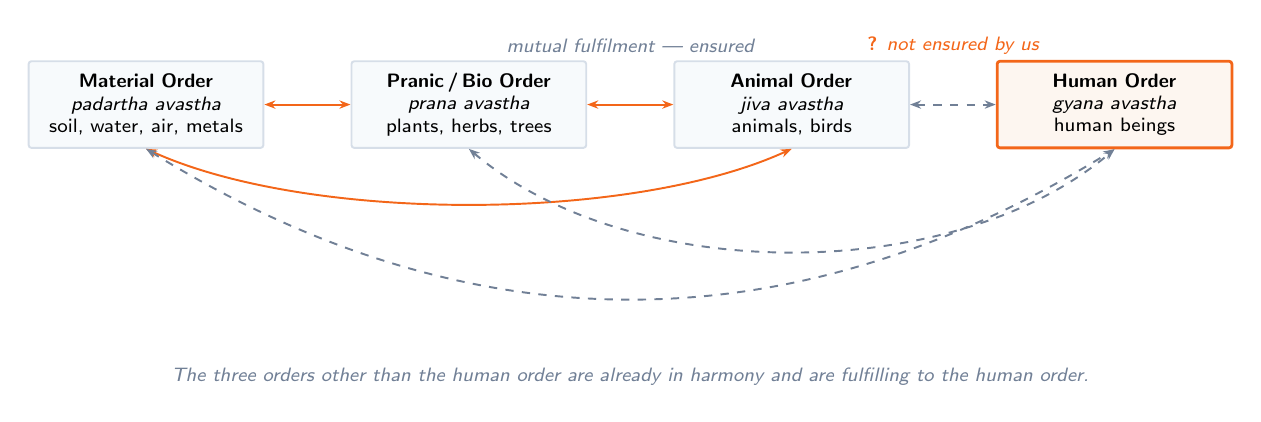
\begin{tikzpicture}[
  font=\sffamily\scriptsize,
  ord/.style={draw=rulegrey,fill=panel,rounded corners=1pt,line width=0.7pt,
              align=center,inner sep=4pt,text width=27mm,minimum height=11mm},
  hum/.style={draw=ocre,fill=tint,rounded corners=1pt,line width=1pt,
              align=center,inner sep=4pt,text width=27mm,minimum height=11mm},
  lbl/.style={font=\sffamily\scriptsize\itshape,text=slatelight},
  mf/.style={{Stealth[length=4pt]}-{Stealth[length=4pt]},line width=0.7pt,
             draw=ocre},
  miss/.style={{Stealth[length=4pt]}-{Stealth[length=4pt]},line width=0.7pt,
               draw=slatelight,dashed}]

\node[ord] (m) at (0,0)    {\textbf{Material Order}\\ \emph{padartha avastha}\\
  soil, water, air, metals};
\node[ord] (p) at (4.1,0)  {\textbf{Pranic\,/\,Bio Order}\\ \emph{prana
  avastha}\\ plants, herbs, trees};
\node[ord] (a) at (8.2,0)  {\textbf{Animal Order}\\ \emph{jiva avastha}\\
  animals, birds};
\node[hum] (h) at (12.3,0) {\textbf{Human Order}\\ \emph{gyana avastha}\\
  human beings};

\draw[mf] (m) -- (p);
\draw[mf] (p) -- (a);
\draw[miss] (a) -- (h);

\draw[mf] (m.south) .. controls (2.05,-1.5) and (6.15,-1.5) .. (a.south);
\draw[miss] (p.south) .. controls (6.15,-2.3) and (10.25,-2.3) .. (h.south);
\draw[miss] (m.south) .. controls (4.1,-3.1) and (8.2,-3.1) .. (h.south);

\node[lbl] at (6.15,0.75) {mutual fulfilment --- ensured};
\node[lbl,text=ocre] at (10.25,0.75) {\textbf{?} not ensured by us};
\node[lbl] at (6.15,-3.45) {The three orders other than the human order are
  already in harmony and are fulfilling to the human order.};
\end{tikzpicture}
\end{center}

\textbf{The harmony among them.} The solid links above are relations of
\textbf{mutual fulfilment} that already hold; the dashed links are the ones
\textbf{we have failed to ensure}.

\begin{apts}
\item \textbf{Material $\leftrightarrow$ Pranic.} The material order provides
      nutrients as soil and minerals; the pranic order decays and enriches the
      soil in return, holds it against erosion, and produces
      oxygen\,/\,carbon dioxide.
\item \textbf{Material, Pranic $\leftrightarrow$ Animal.} The material order
      provides the basis for the movement of animals, birds and fishes; the
      animal order enriches the soil with its excreta and pollinates the
      flowers of the pranic order; the pranic order feeds the animals.
\item \textbf{The three orders $\rightarrow$ Human.} Each of these orders is
      fulfilling to the human order --- verifiable from the multiple uses we
      draw from them.
\item \textbf{Human $\rightarrow$ the three orders: missing.} We too have a
      natural acceptance to be mutually fulfilling to the other three, but
      \textbf{we are not able to ensure it}. We depend on the material order
      but pollute the soil and deplete the fossil fuels; we depend on plants
      but have deforested and destroyed species; we depend on animals but have
      made many extinct.
\end{apts}

\textbf{Conclusion.} There is interconnectedness and mutual fulfilment in all
the orders of nature \textbf{except the human order} --- and that single
missing link is the whole problem, and the whole task. We have not understood
the harmony that exists between the orders, nor our own needs properly, and
have consequently disturbed both ourselves and the balance among the other
three.


\part{Objective Question Bank with Answers}
% ---------------------------------------------------------------------------
%  PART II -- Objective question bank
% ---------------------------------------------------------------------------
\chapter{Objective Question Bank with Answers}
\chaptermark{Objective Question Bank}

Every multiple-choice question, fill-in-the-blank and one-mark short answer
recorded for HS248AT --- \textbf{76 items} in three sections. The
multiple-choice section is arranged \emph{by paper}, because the objective
part of a paper is written against the clock and it helps to know what one
paper's worth of them looks like.

\section{A. Multiple Choice Questions}

\subsection*{A.1\enspace From the CIE quiz papers (with official answers)}
\addcontentsline{toc}{section}{A.1 From the CIE quiz papers}

\begin{objtable}
\qn{1} & What is the fundamental principle of harmony in nature and existence?
  \optsinline{Competition}{Coexistence}{Dominance}{Isolation} &
  \textbf{(b) Coexistence} \\ \hline
\qn{2} & What is the role of human beings in maintaining harmony in nature?
  \optsinline{Exploiting natural resources}{Preserving and nurturing nature}%
  {Dominating other species}{Isolating from the environment} &
  \textbf{(b) Preserving and nurturing nature} \\ \hline
\qn{3} & Which of the following best describes the Physical Order?
  \optsinline{Includes only human-made objects}{Comprises natural elements
  like soil, water, air and minerals}{Refers exclusively to living beings}%
  {Focuses on mental and spiritual aspects} &
  \textbf{(b) Comprises natural elements like soil, water, air and minerals}
  \\ \hline
\qn{4} & What distinguishes the Human Order from the other three orders?
  \optsinline{Physical strength}{Intelligence and moral values}{Ability to
  photosynthesise}{Instinctual behaviour only} &
  \textbf{(b) Intelligence and moral values} \\ \hline
\qn{5} & In the context of coexistence, what is the meaning of `prosperity'?
  \optsinline{Material wealth accumulation}{Holistic well-being and
  happiness}{Physical strength and power}{Technological superiority} &
  \textbf{(b) Holistic well-being and happiness} \\ \hline
\qn{6} & Comprehensive Human Goals include all the following except:
  \optsinline{Resolution}{Prosperity}{Fearlessness (trust)}{Isolation} &
  \textbf{(d) Isolation} \\ \hline
\qn{7} & Gratitude is considered a \blank\ value in relationships.
  \optsinline{Cultural}{Financial}{Universal}{Personal} &
  \textbf{(c) Universal} \\ \hline
\qn{8} & The word ``society'' is primarily used in the context of human
  \blank\ relationship.
  \optsinline{Human}{Nature}{Both}{None} &
  \textbf{(a) Human} \\ \hline
\qn{9} & Prosperity deals with:
  \optsinline{Right understanding in the self}{Fulfilment in relationship}%
  {Ensuring more than required physical facility}{None} &
  \textbf{(c) Ensuring more than required physical facility} \\ \hline
\qn{10} & \blank\ is the feeling of responsibility towards the body of my
  relative.
  \optsinline{Care}{Guidance}{Respect}{Affection} &
  \textbf{(a) Care} (mamata) \\ \hline
\qn{11} & \blank\ means harmony within myself.
  \optsinline{Pleasure}{Happiness}{Excitement}{Fearlessness} &
  \textbf{(b) Happiness} \\ \hline
\qn{12} & The fourth order of nature is \blank.
  \optsinline{Bio order}{Animal order}{Human order}{Material order} &
  \textbf{(c) Human order} \\ \hline
\qn{13} & The continuity of a plant species is maintained in nature by the
  \blank\ method.
  \optsinline{Constitution conformance}{Seed conformance}{Right value \,/\,
  sanskaar}{Breed conformance} &
  \textbf{(b) Seed conformance} \\ \hline
\qn{14} & There is \blank\ among the four orders of nature.
  \optsinline{Inherent struggle}{No dependency}{Mutual fulfilment}%
  {Opposition} &
  \textbf{(c) Mutual fulfilment} \\ \hline
\qn{15} & Our natural acceptance is to live in \blank\ with nature.
  \optsinline{Harmony}{Struggle for survival}{Opposition}{None of the above} &
  \textbf{(a) Harmony} \\ \hline
\qn{16} & Production and work for physical facilities leads to \blank\ in
  family and \blank\ with nature.
  \optsinline{Prosperity, existence}{Happiness, existence}{Happiness,
  co-existence}{Prosperity, co-existence} &
  \textbf{(d) Prosperity, co-existence} \\ \hline
\end{objtable}

\subsection*{A.2\enspace CIE-II --- 7 May 2025}
\addcontentsline{toc}{section}{A.2 CIE-II, 7 May 2025}

\begin{objtable}
\qn{17} & Which of the following is considered the foundation of a strong
  human relationship?
  \optsinline{Intelligence}{Trust}{Wealth}{Appearance} &
  \textbf{(b) Trust} --- the \emph{adhara mulya}, foundation value
  \seeq{31}\seeq{32} \\ \hline
\qn{18} & Disrespect Arising out of
  \begin{optlist}
  \item Lack of communication
  \item Lack of knowledge
  \item Differentiation leading to Discrimination
  \item Lack of Wealth
  \end{optlist} &
  \textbf{(c) Differentiation leading to Discrimination} \seeq{36} \\ \hline
\qn{19} & Care is the feeling
  \begin{optlist}
  \item of responsibility and commitment for nurturing and protection of the
        Body of my relative.
  \item of responsibility and providing facility for nurturing and protection
        of the Body of my relative
  \item of responsibility of making the other feel comfortable with respect to
        Body of my relative
  \item of showing affection to the Body of my relative
  \end{optlist} &
  \textbf{(a)} --- the text defines care (\emph{mamata}) as the feeling to
  \emph{nurture and protect the body of our relative}, taken up as a
  responsibility \seeq{39} \\ \hline
\qn{20} & Fulfilment of relationship means
  \begin{optlist}
  \item Making effort for self development, i.e.\ development of one's own
        competence
  \item Making effort for mutual development, i.e.\ development of one's own
        competence and being of help to the other in developing their
        competence
  \item Making effort for mutual understanding, i.e.\ understanding of one's
        own competence and being of help to the other in understanding their
        competence
  \item Making effort for mutual in acquiring prosperity
  \end{optlist} &
  \textbf{(b) Mutual development} --- the response mode is defined as
  ``a sense of responsibility to improve our own competence and the other's
  competence; we work for mutual fulfilment'' \seeq{48} \\ \hline
\qn{21} & With the complete understanding of respect
  \begin{optlist}
  \item \ldots we all are the same in terms of intelligent, prosperity and
        status.
  \item \ldots we all are the same in terms of Knowledge, family, society.
  \item \ldots we all are the same in terms of competence, prosperity and
        status.
  \item \ldots we all are the same in terms of intention, program and
        potential.
  \end{optlist} &
  \textbf{(d) intention, program and potential} \seeq{35} \\ \hline
\end{objtable}

\begin{note}
\textbf{\sffamily A note on item 21.} The text's own triad is \emph{basic
aspiration} (we both want continuous happiness and prosperity),
\emph{programme of action} (to understand and live in harmony at all four
levels) and \emph{potential} (the activities and powers of the Self are the
same in both). The paper writes ``intention'' where the text writes
``aspiration\,/\,desire'', but option (d) is the only one carrying the triad
at all --- and note that (c) is a deliberate trap: \textbf{competence} is
precisely the one thing in which we are \emph{not} the same.
\end{note}

\subsection*{A.3\enspace Improvement CIE --- June 2025}
\addcontentsline{toc}{section}{A.3 Improvement CIE, June 2025}

\begin{objtable}
\qn{22} & The participation of the human being in ensuring the role of
  physical facility in nurture, protection and providing means for the body is
  called its \blank
  \optsinline{Utility value}{Artistic value}{Activity}{Energy} &
  \textbf{(a) Utility value} \seeq{4} \\ \hline
\qn{23} & When something is active or has activity, it is called as \blank
  \optsinline{space}{unit}{energy}{value} &
  \textbf{(b) unit} --- ``only units are active; when something is active or
  has activity, we call it a unit'' \seeq{65} \\ \hline
\qn{24} & The following are the characteristics of space except \blank
  \optsinline{Unlimited}{No activity}{Energy in equilibrium}{Self-organized} &
  \textbf{(d) Self-organized} --- space is \emph{not} self-organised; it is
  that in which \emph{self-organisation is available} \seeq{61}\seeq{65}
  \\ \hline
\qn{25} & The natural characteristic of material order is \blank
  \optsinline{Composition}{Decomposition}{Composition\slash Decomposition}%
  {Nurture\slash worsen} &
  \textbf{(c) Composition\slash Decomposition} \seeq{52}\seeq{54} \\ \hline
\qn{26} & Conformance of material order is named as \blank
  \optsinline{constitution conformance}{Seed conformance}{Breed conformance}%
  {sanskaar conformance} &
  \textbf{(a) constitution conformance} \seeq{55} \\ \hline
\end{objtable}

\subsection*{A.4\enspace Semester End Examination --- June/July 2025}
\addcontentsline{toc}{section}{A.4 SEE, June/July 2025}

\begin{objtable}
\qn{27} & How does ensuring justice in relationships contribute to society?
  \begin{optlist}
  \item It leads to fearlessness and co-existence
  \item It leads to prosperity and right understanding
  \item It promotes self-regulation and health
  \item It ensures better exchange and storage
  \end{optlist} &
  \textbf{(a) fearlessness and co-existence} --- \emph{Nyaya-Suraksha} is the
  dimension that leads to \emph{abhaya} and \emph{saha-astitva}
  \seeq{44}\seeq{69} \\ \hline
\qn{28} & Imagination is continuous with
  \optsinline{Time}{Soul}{Body}{None} &
  \textbf{(a) Time} --- ``imaging continues with time; it is taking place all
  the time'' \seeq{24} \\ \hline
\qn{29} & Identify the solution which helps human being to transform from
  animal consciousness to human consciousness.
  \optsinline{Right understanding}{Realization}{Value education}{Physical
  facilities} &
  \textbf{(a) Right understanding} --- the transformation is accomplished
  ``only by working for right understanding as the first priority''
  \seeq{22} \\ \hline
\qn{30} & Which of the following is a fundamental human aspiration related to
  relationships?
  \begin{optlist}
  \item Physical comfort.
  \item Financial security.
  \item Mutual understanding and fulfillment.
  \item Accumulating wealth.
  \end{optlist} &
  \textbf{(c) Mutual understanding and fulfillment} \seeq{19} \\ \hline
\qn{31} & Which of the following capacity leads to desires
  \optsinline{Power}{Expectation}{Realization}{Thoughts} &
  \textbf{(c) Realization} --- see the note below \seeq{24} \\ \hline
\qn{32} & Which of the following is considered the foundation of a strong
  human relationship?
  \optsinline{Intelligence}{Trust}{Wealth}{Appearance} &
  \textbf{(b) Trust} \seeq{31}\seeq{32} \\ \hline
\qn{33} & Respect in a relationship means:
  \begin{optlist}
  \item Agreeing to everything
  \item Controlling the other person's actions
  \item Valuing the other person's opinions and boundaries
  \item Always trying to win argument.
  \end{optlist} &
  \textbf{(c) Valuing the other person's opinions and boundaries} --- the
  option nearest to \emph{right evaluation} \seeq{35} \\ \hline
\qn{34} & The participation of the human being in ensuring the role of
  physical facility to help and preserve its utility is called its \blank
  \optsinline{Utility value}{Artistic value}{Activity}{Energy} &
  \textbf{(a) Utility value} \seeq{4} \\ \hline
\qn{35} & A harmonious world is created by values at 4 levels. These are:
  \begin{optlist}
  \item Home, family, society, country
  \item Individual, family, society, universe
  \item School, home, office, temple
  \item None of these
  \end{optlist} &
  \textbf{(b) Individual, family, society, universe} \seeq{5} \\ \hline
\qn{36} & When nature is submerged in space it is known as
  \optsinline{Conformance}{Acceptance}{Mixing}{Co-existence} &
  \textbf{(d) Co-existence} --- see the note below \seeq{62} \\ \hline
\end{objtable}

\begin{note}
\textbf{\sffamily Three items on this paper need care.}

\textbf{Item 31 --- ``which capacity leads to desires''.} The text gives the
self-organised sequence as \textbf{Realization \& Understanding (1, 2)
$\rightarrow$ Desire (3) $\rightarrow$ Thought (4) $\rightarrow$ Expectation
(5)}. On that sequence the capacity that leads to desire is
\textbf{Realization}, and that is the answer to give. Be aware of the trap:
the text \emph{also} describes today's enslaved (\emph{partantra}) flow, in
which the direction is reversed --- sensation sets thoughts, and thoughts set
desires. `Thoughts' is therefore true of how we live now, but `Realization' is
the capacity the text names.

\textbf{Item 35 --- the four levels.} The text's four levels of living are
\emph{individual, family, society, nature\,/\,existence}. The paper's option
(b) writes ``universe'' for nature\,/\,existence; it is nonetheless the only
option carrying the right sequence.

\textbf{Item 36 --- nature submerged in space.} The text's own equation is
\textbf{Existence $=$ Nature submerged in Space}, so the strictly correct word
is \emph{existence}, which is not on offer. Since the text immediately adds
that \textbf{existence is co-existence}, option (d) is the intended answer.
\end{note}

\section{B. Fill in the Blanks and One-Liners}

\begin{objtable}
\qn{1} & \blank\ and Respect are considered the foundational values of a
  relationship. & \textbf{Trust} (vishvas) \\ \hline
\qn{2} & Visualising a universal harmonious order in society includes the idea
  of an \blank\ Society and Universal Order, from family to world family. &
  \textbf{Undivided} (Akhanda Samaja) \\ \hline
\qn{3} & Prosperity and fearlessness (trust) are part of the comprehensive
  human goals in \blank\ in society. &
  \textbf{Right understanding} (samadhana) \\ \hline
\qn{4} & There are \blank\ comprehensive human goals. &
  \textbf{Four} --- right understanding, prosperity, fearlessness (trust),
  co-existence \\ \hline
\qn{5} & The human goal at the level of the individual is \blank. &
  \textbf{Right understanding} (samadhana) \\ \hline
\qn{6} & The human goal at the level of the family is \blank. &
  \textbf{Prosperity} (samriddhi) \\ \hline
\qn{7} & The human goal at the level of society is \blank. &
  \textbf{Fearlessness \,/\, trust} (abhaya) \\ \hline
\qn{8} & The human goal at the level of nature is \blank. &
  \textbf{Co-existence} (saha-astitva) \\ \hline
\qn{9} & Human--human interaction (its recognition, fulfilment and evaluation
  leading to mutual happiness) is called \blank. &
  \textbf{Justice} (nyaya) \\ \hline
\qn{10} & Human--rest-of-nature relation (recognition, fulfilment, evaluation
  leading to mutual prosperity) is called \blank. &
  \textbf{Preservation} (suraksha) --- enrichment, protection, right
  utilisation \\ \hline
\qn{11} & Human values are essential for \blank. &
  \textbf{Harmony at all four levels of living} --- and hence for mutual
  fulfilment and mutual happiness in relationship \\ \hline
\qn{12} & Mutual happiness in human--human interaction leads to \blank. &
  \textbf{Justice} (nyaya) --- mutual happiness ensured is the fourth element
  of justice \\ \hline
\qn{13} & \blank\ is the foundation value (adhara mulya) in relationship. &
  \textbf{Trust} (vishvas) \\ \hline
\qn{14} & What do you understand by complete value? &
  \textbf{Love} (prema) --- the feeling of being related to all; hence called
  \emph{purna mulya} \\ \hline
\qn{15} & The value or participation of different orders in existence is also
  referred to as \blank. &
  \textbf{Natural characteristic} (svabhava) \\ \hline
\qn{16} & \emph{Sah-astitva} means \blank. & \textbf{Co-existence} \\ \hline
\qn{17} & Which activity of the self indicates that ``there is
  complementarity in nature and no opposition''? &
  \textbf{Realization} (and understanding) --- activities 1 and 2 of the Self
  \\ \hline
\qn{18} & Respect means \blank. &
  \textbf{Right evaluation} --- to be evaluated as I am \\ \hline
\qn{19} & The three mistakes in evaluation are \blank, \blank\ and \blank. &
  \textbf{Over evaluation} (adhi-mulyana), \textbf{under evaluation}
  (ava-mulyana), \textbf{otherwise evaluation} (a-mulyana) \\ \hline
\qn{20} & Ensuring justice in relationship, on the basis of values, leads to
  \blank\ in society. &
  \textbf{Fearlessness \,/\, trust} (abhaya) \\ \hline
\qn{21} & The two mechanisms of self-exploration are \blank\ and \blank. &
  \textbf{Natural acceptance} and \textbf{experiential validation} \\ \hline
\qn{22} & Realization and understanding are tested for \blank, \blank\ and
  \blank. &
  \textbf{Assurance, satisfaction and universality} (same for all time, space
  and individual) \\ \hline
\qn{23} & The needs of the Self are \blank\ and \blank; the needs of the Body
  are \blank\ and \blank. &
  \emph{Self:} \textbf{continuous and qualitative}. \emph{Body:}
  \textbf{temporary and quantitative}. \\ \hline
\qn{24} & Sanyama is the basis of \blank. & \textbf{Svasthya} (health)
  \\ \hline
\qn{25} & The five dimensions of human endeavour are \blank. &
  \textbf{Siksha-Sanskara, Svasthya-Sanyama, Nyaya-Suraksha, Utpadana-Karya,
  Vinimaya-Kosha} \\ \hline
\qn{26} & The three aspects of suraksha are \blank. &
  \textbf{Enrichment} (samvardhana), \textbf{Protection} (sanrakshana),
  \textbf{Right utilisation} (sadupayoga) \\ \hline
\qn{27} & Production must be through a \blank\ process, in harmony with
  nature. &
  \textbf{Cyclical} (avartansheel) process --- cyclic, and enriching every
  unit \\ \hline
\qn{28} & Existence $=$ \blank\ $+$ \blank. &
  \textbf{Space $+$ Units} (in space); i.e.\ \textbf{nature submerged in
  space} \\ \hline
\qn{29} & Space is \blank\ energy; units are \blank. &
  Space is \textbf{energy in equilibrium} (constant energy); units are
  \textbf{energised and active} \\ \hline
\qn{30} & Conformance in the four orders is \blank, \blank, \blank\ and
  \blank. &
  \textbf{Constitution, Seed, Breed, Sanskar} conformance \\ \hline
\qn{31} & The innateness of the human order at the level of `I' is \blank. &
  \textbf{The will to live with happiness} \\ \hline
\qn{32} & The svabhava of the self (`I') in human beings is \blank. &
  \textbf{Perseverance} (dhirata), \textbf{bravery} (virata) and
  \textbf{generosity} (udarata) \\ \hline
\qn{33} & SVDD, SSDD and SSSS stand for \blank. &
  \textbf{Sadhan Viheen Dukhi Daridra; Sadhan Sampann Dukhi Daridra; Sadhan
  Sampann Sukhi Samriddha} \\ \hline
\qn{34} & Svatva, Swatantrata and Swarajya mean \blank. &
  \textbf{Innateness; self-organisation} (harmony in oneself);
  \textbf{self-expression} (harmony with others) \\ \hline
\qn{35} & The four elements of justice are \blank. &
  \textbf{Recognition of values, fulfilment, evaluation, mutual happiness
  ensured} \\ \hline
\end{objtable}

\section{C. One-Mark Short Answers}

The Improvement CIE of \textbf{18 June 2026} broke with the earlier pattern:
its Part~A was not multiple choice but five one-mark short-answer questions,
to be written in ten minutes. There is nothing to guess at, so these are worth
rehearsing as written answers.

\begin{objtable}
\qn{1} & Give any two definitions for the term co-existence. \mmk{1} &
  Any two of: \textbf{(i)} to exist together and in mutual tolerance;
  \textbf{(ii)} to learn to recognise and live with difference;
  \textbf{(iii)} a relationship in which none of the parties is trying to
  destroy the other \seeq{63} \\ \hline
\qn{2} & State the four orders of nature. \mmk{1} &
  \textbf{Material} (padartha avastha), \textbf{Pranic\,/\,Bio} (prana
  avastha), \textbf{Animal} (jiva avastha), \textbf{Human\,/\,Knowledge}
  (gyana avastha) \seeq{51} \\ \hline
\qn{3} & Identify the svabhava\,/\,value of the self (`I') in human beings.
  \mmk{1} &
  \textbf{Perseverance} (dhirata), \textbf{bravery} (virata) and
  \textbf{generosity} (udarata) \seeq{54} \\ \hline
\qn{4} & Summarize 2 things that human beings have to do to realize the mutual
  fulfilment in nature. \mmk{1} &
  \textbf{(i) Understand} the harmony and interconnectedness among the four
  orders --- and our own needs --- correctly; \textbf{(ii) live and produce
  accordingly}, through a cyclic (avartansheel) process that enriches every
  unit \seeq{59}\seeq{60} \\ \hline
\qn{5} & Differentiate between Units and Space. \mmk{1} &
  \textbf{Units} are limited, active, energised, recognise and fulfil their
  relation with other units, and are self-organised. \textbf{Space} is
  unlimited and all-pervading, no-activity, energy in equilibrium, reflecting
  and transparent, and self-organisation is available in it \seeq{65}
  \\ \hline
\end{objtable}

\begin{note}
\textbf{\sffamily On item 4.} The text does not give a numbered list of ``two
things'' under that heading. What it does say, in diagnosing why the human
order alone fails to be mutually fulfilling, is that \emph{``we have not
understood the harmony that exists between these orders. We have not even
understood our own needs properly, nor have we understood harmonious ways to
fulfil our needs.''} The two things to do are therefore the two failures put
right: \textbf{understand}, and then \textbf{live and produce accordingly}.
That is the answer given above; it is derived from the text rather than quoted
from a list in it.
\end{note}


\part{The Question Papers}
% ---------------------------------------------------------------------------
%  PART III -- The question papers, reproduced in full
% ---------------------------------------------------------------------------
\chapter{The Question Papers}
\chaptermark{The Question Papers}

The five papers for which full scans survive are reproduced here
question-for-question, in chronological order, exactly as printed --- header,
instructions, question order, numbering, and the three code columns each paper
carried beside its questions.

\vspace{2pt}
Every question also carries a pointer in the last column to the answer
elsewhere in this book, so a whole past paper can be worked end to end and
then marked:

\begin{keybox}
\textbf{Q\emph{n}} \ $\rightarrow$ \ Part~I, descriptive question \emph{n}
\hfill
\textbf{A\emph{n}} \ $\rightarrow$ \ Part~II, multiple-choice item \emph{n}
\newline
\textbf{B\emph{n}} \ $\rightarrow$ \ Part~II, fill-in-the-blank \emph{n}
\hfill
\textbf{C\emph{n}} \ $\rightarrow$ \ Part~II, one-mark short answer \emph{n}
\end{keybox}

The four papers not reproduced here --- SEE October 2023, CIE~1 of 22 June
2024, CIE~2 of 24 July 2024 and SEE September/October 2024 --- are listed
question by question in \textbf{Appendix~A}, with the same pointers. Their
questions are all answered; only the printed paper itself was unavailable.

\section{Improvement CIE --- 28 August 2024}

\begin{papermeta}
\mk{Course code}   & \mv{HS248AT}                    &
\mk{Maximum marks} & \mv{25}                          \\
\mk{Semester}      & \mv{IV}                          &
\mk{Duration}      & \mv{60 minutes}                  \\
\mk{Academic year} & \mv{2023--2024, Even Semester}   &
\mk{Assessment}    & \mv{Improvement CIE --- Quiz and Test} \\
\mk{Date}          & \mv{28 August 2024}              &
\mk{Structure}     & \mv{Part A 5 M \textbf{+} Part B 25 M} \\
\end{papermeta}

\subsection*{Part A --- Objective Questions \hfill 5 Marks}

\begin{qtable}
\qn{1} & What is the fundamental principle of harmony in nature and existence?
  \optsinline{Competition}{Coexistence}{Dominance}{Isolation}
  & 1 & CO3 & L1 & \ap{A1} \\ \hline
\qn{2} & What is the role of human beings in maintaining harmony in nature?
  \begin{optlist}
  \item Exploiting natural resources
  \item Preserving and nurturing nature
  \item Dominating other species
  \item Isolating from the environment
  \end{optlist}
  & 1 & CO2 & L2 & \ap{A2} \\ \hline
\qn{3} & Which of the following best describes the Physical Order?
  \begin{optlist}
  \item Includes only human-made objects
  \item Comprises natural elements like soil, water, air, and minerals
  \item Refers exclusively to living beings
  \item Focuses on mental and spiritual aspects
  \end{optlist}
  & 1 & CO2 & L1 & \ap{A3} \\ \hline
\qn{4} & What distinguishes the Human Order from the other three orders?
  \begin{optlist}
  \item Physical strength
  \item Intelligence and moral values
  \item Ability to photosynthesize
  \item Instinctual behaviour only
  \end{optlist}
  & 1 & CO4 & L1 & \ap{A4} \\ \hline
\qn{5} & In the context of coexistence, what is the meaning of `prosperity'?
  \begin{optlist}
  \item Material wealth accumulation
  \item Holistic well-being and happiness
  \item Physical strength and power
  \item Technological superiority
  \end{optlist}
  & 1 & CO3 & L1 & \ap{A5} \\ \hline
\end{qtable}

\subsection*{Part B --- Descriptive Questions \hfill 25 Marks}

\begin{qtable}
\qn{1} & Existence is co-existence of mutually interacting units in
  all-pervasive space. Explain & 5 & CO3 & L2 & \ap{Q62} \\ \hline
\qn{2} & What is the natural characteristics (swabhava) of human order?
  Explain & 5 & CO2 & L1 & \ap{Q54} \\ \hline
\qn{3} & What are the four orders of nature? Briefly explain them
  & 5 & CO4 & L2 & \ap{Q51} \\ \hline
\qn{4} & How can we say that `nature is Self-Organized and in space
  Self-Organization Is Available.' & 5 & CO4 & L2 & \ap{Q61} \\ \hline
\qn{5} & Explain the difference and similarities between Pranic order and
  animal order. What is the relation between the two orders? & 5 & CO2 & L1 &
  \ap{Q57} \\ \hline
\end{qtable}

\subsection*{Marks distribution as printed}

\begin{mdtable}
Test --- Max Marks & xx & 12 & 07 & 11 & 14 & 16 & xx & xx & xx & xx \\ \hline
\end{mdtable}

\vspace{4pt}
Four cells were left as the template's own \texttt{xx} placeholder and are
reproduced that way. They are all cells that would have been zero: no question
on this paper is mapped to CO1, and none is set above L2.

\begin{note}
\textbf{\sffamily The paper does not add up to its own maximum.} The header
states a maximum of \textbf{25 marks}, but Part~A carries 5 and the five
Part~B questions carry 5 each --- \textbf{30 in total}. The footer table above
agrees with the questions, not with the header: its CO row totals 30
($12+7+11$) and its BT row totals 30 ($14+16$), and both reconcile exactly
with the per-question codes in the two grids. The discrepancy is in the
original and has been left as printed.
\end{note}

\section{CIE-II --- 7 May 2025}

\begin{papermeta}
\mk{Course code}   & \mv{HS248AT}                    &
\mk{Maximum marks} & \mv{25 $+$ 5}                    \\
\mk{Semester}      & \mv{IV}                          &
\mk{Duration}      & \mv{60 minutes}                  \\
\mk{Academic year} & \mv{2024--2025, Even Semester}   &
\mk{Assessment}    & \mv{CIE-II --- Quiz and Test}    \\
\mk{Date}          & \mv{7 May 2025}                  &
\mk{Structure}     & \mv{Part A 5 M \textbf{+} Part B 25 M} \\
\end{papermeta}

This is the only regular CIE in the collection --- the other four papers are
improvement or semester-end sittings. Its subject matter is correspondingly
narrower: every question on it comes from harmony in the family and the values
in relationship, which is the block of the syllabus a second CIE covers.

\subsection*{Part A --- Objective Questions \hfill 5 Marks}

\begin{qtable}
\qn{1} & Which of the following is considered the foundation of a strong human
  relationship?
  \optsinline{Intelligence}{Trust}{Wealth}{Appearance}
  & 1 & CO1 & L1 & \ap{A17} \\ \hline
\qn{2} & Disrespect Arising out of
  \begin{optlist}
  \item Lack of communication
  \item Lack of knowledge
  \item Differentiation leading to Discrimination
  \item Lack of Wealth
  \end{optlist}
  & 1 & CO2 & L1 & \ap{A18} \\ \hline
\qn{3} & Care is the feeling
  \begin{optlist}
  \item of responsibility and commitment for nurturing and protection of the
        Body of my relative.
  \item of responsibility and providing facility for nurturing and protection
        of the Body of my relative
  \item of responsibility of making the other feel comfortable with respect to
        Body of my relative
  \item of showing affection to the Body of my relative
  \end{optlist}
  & 1 & CO2 & L1 & \ap{A19} \\ \hline
\qn{4} & Fulfilment of relationship means
  \begin{optlist}
  \item Making effort for self development, i.e. development of one's own
        competence
  \item Making effort for mutual development, i.e. development of one's own
        competence and being of help to the other in developing their
        competence
  \item Making effort for mutual understanding, i.e. understanding of one's
        own competence and being of help to the other in understanding their
        competence
  \item Making effort for mutual in acquiring prosperity
  \end{optlist}
  & 1 & CO3 & L1 & \ap{A20} \\ \hline
\qn{5} & With the complete understanding of respect
  \begin{optlist}
  \item we can see for every individual on the earth that we all are the same
        in terms of intelligent, prosperity and status.
  \item we can see for every individual on the earth that we all are the same
        in terms of Knowledge, family, society.
  \item we can see for every individual on the earth that we all are the same
        in terms of competence, prosperity and status.
  \item we can see for every individual on the earth that we all are the same
        in terms of intention, program and potential.
  \end{optlist}
  & 1 & CO1 & L1 & \ap{A21} \\ \hline
\end{qtable}

\subsection*{Part A --- marks distribution as printed}

\begin{mdtable}
Test --- Max Marks & 2 & 2 & 1 & --- & 5 & --- & --- & --- & --- & --- \\
\hline
\end{mdtable}

\subsection*{Part B --- Descriptive Questions \hfill 25 Marks}

\begin{qtable}
\qn{1} & Justify the following (i)~Relation ship is between one Self (I1) and
  another Self (I2), (ii)~feelings in relationship --- in one Self (I1) for the
  other Self (I2) & 2$+$3 & CO1 & L1 & \ap{Q27} \\ \hline
\qn{2} & Distinguish between Intention and Competence with respect Trust with
  suitable example & 5 & CO3 & L2 & \ap{Q32} \\ \hline
\qn{3} & The complete content of respect is to be able to see that `the other
  is similar to me and we are complementary'. Define complementary in this
  context. & 5 & CO1 & L1 & \ap{Q67} \\ \hline
\qn{4} & Disrespect arises out of differentiation leading to discrimination on
  the basis of body, physical facility or beliefs. illustrate With an example
  & 5 & CO2 & L2 & \ap{Q36} \\ \hline
\qn{5} & Illustrate the natural acceptance values in relationship with an
  example for each (i)~Reverence (ii)~Glory & 5 & CO3 & L1 & \ap{Q39}
  \\ \hline
\end{qtable}

\subsection*{Part B --- marks distribution as printed}

\begin{mdtable}
Test --- Max Marks & 10 & 10 & 5 & --- & 15 & 10 & --- & --- & --- & --- \\
\hline
\end{mdtable}

\section{Improvement CIE --- June 2025}

\begin{papermeta}
\mk{Course code}   & \mv{HS248AT}                    &
\mk{Maximum marks} & \mv{30}                          \\
\mk{Semester}      & \mv{IV}                          &
\mk{Duration}      & \mv{60 minutes}                  \\
\mk{Academic year} & \mv{2024--2025, Even Semester}   &
\mk{Assessment}    & \mv{Improvement CIE --- Quiz and Test} \\
\mk{Date}          & \mv{June 2025}                   &
\mk{Structure}     & \mv{Quiz 5 M \textbf{+} Test 25 M}  \\
\mk{Set by}        & \mv{Department of Mechanical Engineering} &
                   & \\
\end{papermeta}

\subsection*{Quiz \hfill 5 Marks}

\begin{qtable}
\qn{1} & The participation of the human being in ensuring the role of physical
  facility in nurture, protection and providing means for the body is called
  its \blank
  \optsinline{Utility value}{Artistic value}{Activity}{Energy}
  & 1 & CO1 & L2 & \ap{A22} \\ \hline
\qn{2} & When something is active or has activity, it is called as \blank
  \optsinline{space}{unit}{energy}{value}
  & 1 & CO2 & L3 & \ap{A23} \\ \hline
\qn{3} & The following are the characteristics of space except \blank
  \optsinline{Unlimited}{No activity}{Energy in equilibrium}{Self-organized}
  & 1 & CO1 & L1 & \ap{A24} \\ \hline
\qn{4} & The natural characteristic of material order is \blank
  \optsinline{Composition}{Decomposition}{Composition/Decomposition}%
  {Nurture/worsen}
  & 1 & CO1 & L1 & \ap{A25} \\ \hline
\qn{5} & Conformance of material order is named as \blank
  \optsinline{constitution conformance}{Seed conformance}{Breed conformance}%
  {sanskaar conformance}
  & 1 & CO3 & L3 & \ap{A26} \\ \hline
\end{qtable}

\subsection*{Test \hfill 25 Marks}

\begin{qtable}
\qn{1} & Explain the classification of units into Four Orders and the harmony
  among them with the help of a schematic diagram. & 6 & CO1 & L2 &
  \ap{Q74} \\ \hline
\qn{2} & What do you mean by `conformance'? Explain the conformance in the
  four orders. & 6 & CO2 & L4 & \ap{Q55} \\ \hline
\qn{3} & Explain how there is recyclability and self-regulation in nature.
  & 6 & CO3 & L3 & \ap{Q60} \\ \hline
\qn{4} & Elaborate the terms `units' and `space' and mention their
  characteristics. & 7 & CO4 & L4 & \ap{Q65} \\ \hline
\end{qtable}

\subsection*{Marks distribution as printed}

\begin{mdtable}
Test --- Marks & 9 & 7 & 7 & 7 & 3 & 7 & 7 & 13 & --- & --- \\ \hline
\end{mdtable}

\vspace{4pt}
Both rows total 30, which is the paper's maximum. Note that L4 alone carries
13 of the 30 marks: this is an analytical paper, and the six- and seven-mark
questions on conformance and on units and space are where those marks sit.

\section{Semester End Examination --- June/July 2025}
\sectionmark{SEE --- June/July 2025}

\begin{papermeta}
\mk{Course code}   & \mv{HS248AT}                    &
\mk{Maximum marks} & \mv{50}                          \\
\mk{Semester}      & \mv{IV}                          &
\mk{Duration}      & \mv{2 hours}                     \\
\mk{Examination}   & \mv{IV Semester B.E. Regular / Supplementary} &
\mk{Assessment}    & \mv{Semester End Examination}    \\
\mk{Date}          & \mv{June/July 2025}              &
\mk{Applies to}    & \mv{Common to all programs}      \\
\end{papermeta}

\begin{note}
\textbf{\sffamily Instructions to the students, as printed.}
\begin{enumerate}[leftmargin=1.6em,itemsep=2pt,topsep=4pt]
\item Answer all questions from Part A. Part A questions should be answered in
      first three pages of the answer book only.
\item Answer THREE full questions from Part B. In Part B question number 2 is
      compulsory. Answer any one full question from 3 and 4 \& 5 and 6.
\end{enumerate}
\end{note}

The blueprint is worth reading off the instructions before the questions.
Part~A is ten compulsory one-mark objective questions. Part~B sets
\textbf{Q2 compulsory} (14 marks), then \textbf{one of Q3 or Q4} (13 marks) and
\textbf{one of Q5 or Q6} (13 marks) --- three full questions, 40 marks, and two
genuine choices to make in the hall.

\subsection*{Part A --- Compulsory Objective Questions \hfill 10 Marks}

\begin{qtable}
\qn{1.1} & How does ensuring justice in relationships contribute to society?
  \begin{optlist}
  \item It leads to fearlessness and co-existence
  \item It leads to prosperity and right understanding
  \item It promotes self-regulation and health
  \item It ensures better exchange and storage
  \end{optlist}
  & 01 & CO3 & L1 & \ap{A27} \\ \hline
\qn{1.2} & Imagination is continuous with
  \optsinline{Time}{Soul}{Body}{None}
  & 01 & CO1 & L1 & \ap{A28} \\ \hline
\qn{1.3} & Identify the solution which helps human being to transform from
  animal consciousness to human consciousness.
  \optsinline{Right understanding}{Realization}{Value education}%
  {Physical facilities.}
  & 01 & CO1 & L1 & \ap{A29} \\ \hline
\qn{1.4} & Which of the following is a fundamental human aspiration related to
  relationships?
  \begin{optlist}
  \item Physical comfort.
  \item Financial security.
  \item Mutual understanding and fulfillment.
  \item Accumulating wealth.
  \end{optlist}
  & 01 & CO2 & L2 & \ap{A30} \\ \hline
\qn{1.5} & Which of the following capacity leads to desires
  \optsinline{Power}{Expectation}{Realization}{Thoughts}
  & 01 & CO2 & L1 & \ap{A31} \\ \hline
\qn{1.6} & Which of the following is considered the foundation of a strong
  human relationship?
  \optsinline{Intelligence}{Trust}{Wealth}{Appearance}
  & 01 & CO1 & L2 & \ap{A32} \\ \hline
\qn{1.7} & Respect in a relationship means:
  \begin{optlist}
  \item Agreeing to everything
  \item Controlling the other person's actions
  \item Valuing the other person's opinions and boundaries
  \item Always trying to win argument.
  \end{optlist}
  & 01 & CO3 & L1 & \ap{A33} \\ \hline
\qn{1.8} & The participation of the human being in ensuring the role of
  physical facility to help and preserve its utility is called its \blank
  \optsinline{Utility value}{Artistic value}{Activity}{Energy}
  & 01 & CO3 & L2 & \ap{A34} \\ \hline
\qn{1.9} & A harmonious world is created by values at 4 levels. These are:
  \begin{optlist}
  \item Home, family, society, country
  \item Individual, family, society, universe
  \item School, home, office, temple
  \item None of these
  \end{optlist}
  & 01 & CO1 & L1 & \ap{A35} \\ \hline
\qn{1.10} & When nature is submerged in space it is known as
  \optsinline{Conformance}{Acceptance}{Mixing}{Co-existence}
  & 01 & CO3 & L2 & \ap{A36} \\ \hline
\end{qtable}

\subsection*{Part B --- Descriptive Questions \hfill 40 Marks}

\vspace{2pt}
\textbf{\sffamily\color{slate}Question 2 --- compulsory}

\begin{qtable}
\qn{2a} & What do you understand by the value of an entity? What is the value
  of a human being? & 08 & CO1 & L2 & \ap{Q4} \\ \hline
\qn{2b} & For human being physical facility is necessary, but relationship is
  also necessary: Justify with an example comparing with animal order.
  & 06 & CO2 & L4 & \ap{Q21} \\ \hline
\end{qtable}

\vspace{4pt}
\textbf{\sffamily\color{slate}Questions 3 and 4 --- answer any one full
question}

\begin{qtable}
\qn{3a} & ``Discuss how right understanding in relationships contributes to
  harmony in the family. Analyze the role of trust, respect, and
  responsibility in maintaining family unity, and provide examples to support
  your answer.'' & 07 & CO4 & L4 & \ap{Q68} \\ \hline
\qn{3b} & Articulate the four goals of human beings living in a society.
  Critically examine the state of the society today in context with the
  fulfilment of a comprehensive human goal. & 06 & CO3 & L3 &
  \ap{Q41}\newline\ap{Q43} \\ \hline
\orband
\qn{4a} & How do justice and preservation contribute to a harmonious society?
  Analyze the shortcomings of focusing solely on punishment in cases of
  injustice, and explain how true preservation ensures prosperity and
  coexistence with nature. & 06 & CO3 & L4 & \ap{Q69} \\ \hline
\qn{4b} & Explain the concept of harmony in the family. Why is it important,
  and how can it be achieved through right understanding and mutual
  relationships? & 07 & CO3 & L2 & \ap{Q70} \\ \hline
\end{qtable}

\vspace{4pt}
\textbf{\sffamily\color{slate}Questions 5 and 6 --- answer any one full
question}

\begin{qtable}
\qn{5a} & What is sanskaar? Explain its effects or the conformance of the
  human order. & 06 & CO4 & L4 & \ap{Q55} \\ \hline
\qn{5b} & What is the svabhava (natural characteristic) of a unit? Mention the
  natural characteristics of the material, pranic, animal and human orders.
  Give examples & 07 & CO4 & L3 & \ap{Q54} \\ \hline
\orband
\qn{6a} & What do you mean by `conformance'? Explain the conformance in the
  four orders. & 07 & CO3 & L4 & \ap{Q55} \\ \hline
\qn{6b} & Explain the meaning of co-existence. & 06 & CO3 & L3 & \ap{Q63}
  \\ \hline
\end{qtable}

\section{Improvement CIE --- 18 June 2026}

\begin{papermeta}
\mk{Course code}   & \mv{HS248AT}                    &
\mk{Maximum marks} & \mv{05 $+$ 25}                   \\
\mk{Semester}      & \mv{IV}                          &
\mk{Duration}      & \mv{10 min $+$ 60 min}           \\
\mk{Date}          & \mv{18 June 2026}                &
\mk{Assessment}    & \mv{Improvement CIE --- Quiz $+$ Test} \\
\mk{Structure}     & \mv{Part A 5 M \textbf{+} Part B 25 M} &
\mk{Format}        & \mv{Short answer, not multiple choice} \\
\end{papermeta}

This paper breaks the pattern of the earlier improvement CIEs in one respect
worth noting: \textbf{Part~A is not multiple choice}. It sets five one-mark
short-answer questions to be written in ten minutes --- definitions, lists and
one-line differentiations. There is nothing to guess at.

\subsection*{Part A --- Short Answer Questions \hfill 5 Marks}

\begin{qtable}
\qn{1} & Give any two definitions for the term co-existence.
  & 1 & CO1 & L1 & \ap{C1} \\ \hline
\qn{2} & State the four orders of nature. & 1 & CO2 & L1 & \ap{C2} \\ \hline
\qn{3} & Identify the svabhava\,/\,value of the self (`I') in human beings.
  & 1 & CO2 & L2 & \ap{C3} \\ \hline
\qn{4} & Summarize 2 things that human beings have to do to realize the mutual
  fulfilment in nature. & 1 & CO3 & L2 & \ap{C4} \\ \hline
\qn{5} & Differentiate between Units and Space. & 1 & CO4 & L2 & \ap{C5}
  \\ \hline
\end{qtable}

\subsection*{Part B --- Descriptive Questions \hfill 25 Marks}

\begin{qtable}
\qn{1} & Describe how harmony is achieved among the four orders of nature.
  & 5 & CO4 & L2 & \ap{Q59}\newline\ap{Q74} \\ \hline
\qn{2} & Justify that requirement of any order is already available in
  abundance in nature. & 5 & CO3 & L4 & \ap{Q72} \\ \hline
\qn{3} & Demonstrate how interconnectedness, self-regulation and mutual
  fulfilment are among the four orders of nature with an example.
  & 5 & CO2 & L3 & \ap{Q59}\newline\ap{Q60} \\ \hline
\qn{4} & Summarize how the domain of consciousness helps in accomplishing
  development or permanent change. & 5 & CO4 & L2 & \ap{Q73} \\ \hline
\qn{5} & Outline 2 types of units with examples. & 5 & CO3 & L2 & \ap{Q71}
  \\ \hline
\end{qtable}

\subsection*{Marks distribution as printed}

\begin{mdtable}
Test --- Max Marks & 1 & 7 & 11 & 11 & 2 & 18 & 5 & 5 & --- & --- \\ \hline
\end{mdtable}

\vspace{4pt}
Both rows total 30. L2 carries 18 of the 30 marks, which is the mirror image of
the June 2025 paper: this one rewards clear explanation rather than analysis.


\appendix
\renewcommand{\chapkind}{APPENDIX}
% ---------------------------------------------------------------------------
%  APPENDICES
% ---------------------------------------------------------------------------
\chapter{Past-Paper Index --- Where Each Question Has Appeared}
\chaptermark{Past-Paper Index}

The five papers with surviving scans are reproduced in full in Part~III. This
appendix indexes the \textbf{other four} question by question, with the same
pointers to the answers --- \textbf{Q\emph{n}} for Part~I, \textbf{A\emph{n}}
\,/\, \textbf{B\emph{n}} \,/\, \textbf{C\emph{n}} for the three sections of
Part~II. It closes with a one-line summary of all nine papers.

\section*{A.1\enspace CIE 1 --- 22 June 2024 \ \ \normalfont\small(HS248AT,
  25 marks)}
\addcontentsline{toc}{section}{A.1 CIE 1, 22 June 2024}

\begin{idxtable}
\qn{1} & Define self-exploration. What is the content of self-exploration? &
  5 & \ap{Q8} \\ \hline
\qn{2} & ``Right understanding $+$ Relationship $=$ Mutual fulfilment; Right
  understanding $+$ Physical facilities $=$ Mutual prosperity.'' Illustrate
  with two examples for each. & 8 & \ap{Q20} \\ \hline
\qn{3} & How can we ensure harmony in self (`I')? & 4 & \ap{Q24} \\ \hline
\qn{4} & How do prosperity and wealth differ? What is more acceptable to us
  and why? & 8 & \ap{Q16} \\ \hline
\end{idxtable}

\section*{A.2\enspace CIE 2 --- 24 July 2024 \ \ \normalfont\small(HS248AT,
  5 $+$ 25 marks)}
\addcontentsline{toc}{section}{A.2 CIE 2, 24 July 2024}

\begin{idxtable}
\qn{A1--5} & Quiz: foundational values; undivided society; comprehensive human
  goals; gratitude & 5 & \ap{A6--A16} \\ \hline
\qn{B1} & What is the difference between respect and disrespect? Which of the
  two is naturally acceptable to you? & 5 & \ap{Q37} \\ \hline
\qn{B2} & How does affection lead to harmony in the family? & 5 & \ap{Q38}
  \\ \hline
\qn{B3} & What is the meaning of justice in human relationships? How does it
  follow from family to world family? & 5 & \ap{Q29} \\ \hline
\qn{B4} & What do you understand by trust? Differentiate between intention and
  competence with examples. & 5 & \ap{Q32} \\ \hline
\qn{B5} & Explain the comprehensive human goal. How does fearlessness follow
  from right understanding and prosperity? & 5 & \ap{Q42} \\ \hline
\end{idxtable}

\section*{A.3\enspace SEE --- September/October 2024 and October 2023
  \ \ \normalfont\small(50 marks)}
\addcontentsline{toc}{section}{A.3 SEE, Sept/Oct 2024 and Oct 2023}

Where a slot carries two questions, the second is the alternative set in the
other year's paper. Both are answered.

\begin{idxtable}
\qn{1.1--1.10} & Part A --- objective & 10 & \ap{A1--A16} \\ \hline
\qn{2a} & ``To be in a state of harmony is happiness.'' Explain and illustrate
  with two examples. & 6 & \ap{Q14} \\ \hline
\qn{2a\,alt} & Explain the process of self-exploration with a diagram. & 6 &
  \ap{Q9} \\ \hline
\qn{2b} & What do you mean by values? How do they differ from skills? How are
  values and skills complementary? & 6 & \ap{Q6} \\ \hline
\qn{2b\,alt} & What is value education? Describe the need for value education
  with its guidelines. & 6 & \ap{Q1}\newline\ap{Q2}\newline\ap{Q3} \\ \hline
\qn{3a} & What is the role of the value system in family harmony? & 5 &
  \ap{Q48} \\ \hline
\qn{3a\,alt} & Explain the problems faced due to differentiation in
  relationship. & 5 & \ap{Q36} \\ \hline
\qn{3b} & ``Discrimination leads to acrimony in relationships.'' Explain. What
  problems are created when we discriminate? & 5 & \ap{Q36} \\ \hline
\qn{3b\,alt} & What is `justice'? What are its four elements? Is it a
  continuous or a temporary need? & 5 & \ap{Q28} \\ \hline
\qn{3c} & Define love. How can you say that love is the complete value? & 4 &
  \ap{Q40} \\ \hline
\qn{4a} & What do you understand by trust? Differentiate between intention and
  competence with examples. & 5 & \ap{Q32} \\ \hline
\qn{4a\,alt} & Distinguish between the needs of the Self and the needs of the
  Body. & 5 & \ap{Q23} \\ \hline
\qn{4b} & Realization and understanding are essential for happiness and
  harmony. Explain. & 5 & \ap{Q26} \\ \hline
\qn{4b\,alt} & The feeling of love lays down the basis of an undivided
  society. Explain. & 5 & \ap{Q40} \\ \hline
\qn{4c} & Describe the concept of an undivided society and the universal
  order, and explain how both can help create a world family. & 5 & \ap{Q46}
  \\ \hline
\qn{4c\,alt} & Bring out the differences between respect and differentiation.
  & 4 & \ap{Q37} \\ \hline
\qn{5a} & Existence is co-existence of mutually interacting units in
  all-pervasive space. Explain. \,/\, Describe briefly the nature of
  co-existence. & 5 & \ap{Q62}\newline\ap{Q63} \\ \hline
\qn{5b} & Define harmony in nature and why is it important. Explain with
  examples. & 5 & \ap{Q50} \\ \hline
\qn{5b\,alt} & What are the four orders of nature? Briefly explain them. & 5 &
  \ap{Q51} \\ \hline
\qn{5c} & What do you mean by co-existence? & 4 & \ap{Q63} \\ \hline
\qn{6a} & What is the natural characteristic (swabhava) of the human order?
  Explain. & 5 & \ap{Q54} \\ \hline
\qn{6b} & What are the four orders of nature? Briefly explain them. & 5 &
  \ap{Q51} \\ \hline
\qn{6c} & How can we say that `nature is Self-Organized and in space
  Self-Organization is Available'? & 4 & \ap{Q61} \\ \hline
\qn{5c\,/\,6b}\newline\qn{(2023)} & \emph{Holistic technology}; \emph{ethical
  human conduct in terms of values, policy and character}; \emph{nature of the
  universal human order} & 4--5 & --- \\ \hline
\end{idxtable}

\begin{note}
\textbf{\sffamily The one gap in this book, stated plainly.} The last row
above belongs to \textbf{Chapters 11--13}, which are \emph{not} part of the
Unit I--III material supplied for this course. \emph{Holistic technology} and
\emph{ethical human conduct in terms of values, policy and character} are
therefore \textbf{not answered here} --- no source was provided for them, and
answering from outside the prescribed material would break the rule this book
is written under. (The third of the three, the \emph{nature of the universal
human order}, is within scope and is answered in \textbf{Q46}.) If those two
topics are in your syllabus this year, get them from the Chapter 11--13
notes.
\end{note}

\section*{A.4\enspace All nine papers at a glance}
\addcontentsline{toc}{section}{A.4 All nine papers at a glance}

\renewcommand{\arraystretch}{1.35}
\arrayrulecolor{rulegrey}
\begin{tabular}{@{}P{44mm} P{30mm} C{18mm} C{22mm} P{34mm}@{}}
\rowcolor{slate}
\hdr{Assessment} & \hdr{Date} & \hdr{Max M} & \hdr{Questions} & \hdr{Where}
  \\ \hline
SEE (21HSU48) & October 2023 & 50 & 23 & Appendix A.3 \\ \hline
CIE 1 & 22 June 2024 & 25 & 4 & Appendix A.1 \\ \hline
CIE 2 & 24 July 2024 & 5 $+$ 25 & 10 & Appendix A.2 \\ \hline
Improvement CIE \,/\, CIE 3 & 28 August 2024 & 25 & 10 &
  \textbf{Part III, \S1} \\ \hline
SEE & Sept/Oct 2024 & 50 & 23 & Appendix A.3 \\ \hline
CIE-II & 7 May 2025 & 25 $+$ 5 & 10 & \textbf{Part III, \S2} \\ \hline
Improvement CIE & June 2025 & 30 & 9 & \textbf{Part III, \S3} \\ \hline
\textbf{SEE} Regular \,/\, Suppl. & June/July 2025 & 50 & 20 &
  \textbf{Part III, \S4} \\ \hline
Improvement CIE & 18 June 2026 & 05 $+$ 25 & 10 & \textbf{Part III, \S5}
  \\ \hline
\end{tabular}

\chapter{Questions Set More Than Once}
\chaptermark{Questions Set More Than Once}

Across the nine papers, ten topics have been examined two, three or four
times. They are listed below with every occurrence. \textbf{This is the single
most useful page in the book if revision time is short} --- between them these
ten topics account for well over a third of every mark ever set on this
course.

\vspace{2pt}
Watch what happens to the marks and the Bloom's level as a question moves
between papers. \emph{Conformance in the four orders} was worth 6 marks on a
CIE and 7 on the SEE, at L4 both times: the semester-end paper wanted the same
analysis, one point longer. That is the general pattern --- a repeat keeps its
level and gains a mark or two on the way to the SEE. The exception is the
\textbf{18 June 2026} paper, which took three long-answer staples and set them
as \emph{one-mark} short answers; the same material, compressed to a single
line.

\renewcommand{\arraystretch}{1.35}
\arrayrulecolor{rulegrey}
\setlength{\LTpre}{8pt}\setlength{\LTpost}{4pt}
\begin{longtable}{P{58mm} P{80mm} C{14mm}}
\rowcolor{slate}
\hdr{Topic} & \hdr{Set in} & \hdr{Answer} \\ \hline \endfirsthead
\rowcolor{slate}
\hdr{Topic} & \hdr{Set in} & \hdr{Answer} \\ \hline \endhead
\textbf{The four orders of nature} --- set five times, at four different
  lengths: a five-mark explanation, a six-mark version with a schematic
  diagram, and a one-mark list &
  Improvement CIE, 28 Aug 2024, Part B Q3 (5 M)\newline
  SEE, Sept/Oct 2024, Q5b\,alt and Q6b (5 M)\newline
  Improvement CIE, Jun 2025, Test Q1 (6 M)\newline
  Improvement CIE, 18 Jun 2026, Part A Q2 (1 M) &
  \ap{Q51}\newline\ap{Q74}\newline\ap{C2} \\ \hline
\textbf{Svabhava --- the natural characteristic} --- narrowed and widened
  across four papers: the human order alone, then all four orders, then the
  self &
  Improvement CIE, 28 Aug 2024, Part B Q2 (5 M)\newline
  SEE, Sept/Oct 2024, Q6a (5 M)\newline
  SEE, Jun/Jul 2025, Q5b (07 M)\newline
  Improvement CIE, 18 Jun 2026, Part A Q3 (1 M) &
  \ap{Q54}\newline\ap{C3} \\ \hline
\textbf{Co-existence} --- the four-mark definition, the five-mark
  ``mutually interacting units'' version, and the one-mark ``two
  definitions'' &
  Improvement CIE, 28 Aug 2024, Part B Q1 (5 M)\newline
  SEE, Sept/Oct 2024, Q5a and Q5c (5 M, 4 M)\newline
  SEE, Jun/Jul 2025, Q6b (06 M)\newline
  Improvement CIE, 18 Jun 2026, Part A Q1 (1 M) &
  \ap{Q62}\newline\ap{Q63}\newline\ap{C1} \\ \hline
\textbf{`Conformance', and conformance in the four orders} --- identical
  wording twice, plus the \emph{sanskaar} variant &
  Improvement CIE, Jun 2025, Test Q2 (6 M, CO2, L4)\newline
  SEE, Jun/Jul 2025, Q5a --- ``What is sanskaar?'' (06 M, L4)\newline
  SEE, Jun/Jul 2025, Q6a (07 M, CO3, L4) &
  \ap{Q55} \\ \hline
\textbf{Trust --- intention versus competence} --- identical wording all
  three times &
  CIE 2, 24 Jul 2024, Q B4 (5 M)\newline
  SEE, Sept/Oct 2024, Q4a (5 M)\newline
  CIE-II, 7 May 2025, Part B Q2 (5 M) &
  \ap{Q32} \\ \hline
\textbf{Differentiation and discrimination in relationship} &
  CIE 2 \,/\, SEE, Q3a\,alt and Q3b (5 M)\newline
  CIE-II, 7 May 2025, Part B Q4 (5 M) &
  \ap{Q36} \\ \hline
\textbf{Units and space} --- a seven-mark elaboration, then a one-mark
  differentiation &
  Improvement CIE, Jun 2025, Test Q4 (7 M, CO4, L4)\newline
  Improvement CIE, 18 Jun 2026, Part A Q5 (1 M, CO4, L2) &
  \ap{Q65}\newline\ap{C5} \\ \hline
\textbf{Nature is self-organised; in space self-organisation is available} &
  Improvement CIE, 28 Aug 2024, Part B Q4 (5 M)\newline
  SEE, Sept/Oct 2024, Q6c (4 M) &
  \ap{Q61} \\ \hline
\textbf{Trust as the foundation of relationship} (objective) --- identical
  wording and identical options &
  CIE-II, 7 May 2025, Part A Q1 (1 M, CO1, L1)\newline
  SEE, Jun/Jul 2025, Q1.6 (01 M, CO1, L2) &
  \ap{A17}\newline\ap{A32} \\ \hline
\textbf{Utility value of physical facility} (objective) --- reworded:
  \emph{`in nurture, protection and providing means for the body'} became
  \emph{`to help and preserve its utility'}; the four options are unchanged &
  Improvement CIE, Jun 2025, Quiz Q1 (1 M, CO1, L2)\newline
  SEE, Jun/Jul 2025, Q1.8 (01 M, CO3, L2) &
  \ap{A22}\newline\ap{A34} \\ \hline
\textbf{Love as the complete value, and the undivided society} &
  SEE, Sept/Oct 2024, Q3c (4 M)\newline
  SEE, Sept/Oct 2024, Q4b\,alt (5 M) &
  \ap{Q40} \\ \hline
\textbf{Respect versus disrespect \,/\, differentiation} &
  CIE 2, 24 Jul 2024, Q B1 (5 M)\newline
  SEE, Sept/Oct 2024, Q4c\,alt (4 M) &
  \ap{Q37} \\ \hline
\end{longtable}

\chapter{Last-Minute Revision Priorities}
\chaptermark{Revision Priorities}

If you have one evening, work through this list and nothing else. Everything
on it has been set at least twice, or is the skeleton that several other
answers hang from.

\section*{C.1\enspace Unit I}
\addcontentsline{toc}{section}{C.1 Unit I}

\begin{abul}
\item The \textbf{five needs} for value education \seeq{2} and the
      \textbf{five guidelines} \seeq{3}.
\item The \textbf{process of self-exploration} --- the diagram, both
      mechanisms, and the three tests (assurance, satisfaction, universality)
      \seeq{9}.
\item The \textbf{five characteristics of natural acceptance} \seeq{13}.
\item \textbf{Prosperity versus wealth} --- the full comparison table
      \seeq{16}. Set for 8 marks twice.
\item \textbf{Right understanding $+$ relationship} and \textbf{right
      understanding $+$ physical facilities}, with two examples each
      \seeq{20}.
\item The \textbf{Self versus Body needs} table --- six rows \seeq{23}.
\item The \textbf{four-step process} for harmony in `I' \seeq{24}.
\end{abul}

\section*{C.2\enspace Unit II}
\addcontentsline{toc}{section}{C.2 Unit II}

\begin{abul}
\item \textbf{Justice and its four elements}, and that it is a
      \emph{continuous} need \seeq{28}. Follow the official scheme, not the
      legal categories --- see the warning in \emph{How This Book Is
      Arranged} if you have not read it.
\item \textbf{Intention versus competence}, with the friend-on-campus example
      \seeq{32}. Set three times.
\item \textbf{Respect as right evaluation}, and the \textbf{three mistakes}
      --- over, under, otherwise \seeq{35}.
\item The \textbf{differentiation table} --- body \,/\, physical facilities
      \,/\, beliefs, with the problems each creates \seeq{36}.
\item The \textbf{nine values} with their one-line definitions, and which one
      is the foundation value and which the complete value \seeq{31}.
\item The \textbf{comprehensive human goal} and its sequence: right
      understanding $\rightarrow$ prosperity $\rightarrow$ fearlessness
      $\rightarrow$ co-existence \seeq{41}.
\item The \textbf{five dimensions of human endeavour} and what each leads to
      \seeq{44}.
\end{abul}

\section*{C.3\enspace Unit III}
\addcontentsline{toc}{section}{C.3 Unit III}

\begin{abul}
\item \textbf{The single four-orders table} --- things, activity, innateness,
      svabhava, basic activity, conformance \seeq{52}. Most of Unit~III is a
      row or a column of this one table; if you memorise nothing else,
      memorise this.
\item \textbf{Existence $=$ space $+$ units}, and the five-row units-versus-
      space comparison \seeq{62}\seeq{65}.
\item \textbf{Self-organisation} --- units are self-organised; in space,
      self-organisation is \emph{available} \seeq{61}.
\item \textbf{Recyclability and self-regulation}, with the forest and breed
      examples \seeq{60}.
\item \textbf{Interconnectedness and mutual fulfilment} --- and the fact that
      the \emph{human order is the one missing link} \seeq{59}\seeq{74}.
\item \textbf{The two types of units} --- material (jada, gathansheel) and
      conscious (chaitanya, gathanpurna) \seeq{71}, and why development can
      only happen in the second \seeq{73}.
\end{abul}

\section*{C.4\enspace If you have ten minutes}
\addcontentsline{toc}{section}{C.4 If you have ten minutes}

\begin{keybox}
\textbf{Four definitions, verbatim.}
\begin{enumerate}[leftmargin=1.8em,itemsep=2pt,topsep=3pt]
\item \textbf{Trust} --- to be assured that each human being inherently wants
      oneself and the other to be happy and prosperous. \emph{The foundation
      value.}
\item \textbf{Respect} --- right evaluation; to be evaluated as I am.
\item \textbf{Justice} --- recognition of values, fulfilment, evaluation, and
      mutual happiness ensured.
\item \textbf{Prosperity} --- the feeling of having or making available
      \emph{more than the required} physical facilities.
\end{enumerate}

\vspace{3pt}
\textbf{Three sequences.}
\begin{enumerate}[leftmargin=1.8em,itemsep=2pt,topsep=3pt]
\item Right Understanding $\rightarrow$ Prosperity $\rightarrow$ Fearlessness
      $\rightarrow$ Co-existence \quad \emph{(comprehensive human goal)}
\item Realization \& Understanding $\rightarrow$ Desire $\rightarrow$ Thought
      $\rightarrow$ Expectation \quad \emph{(harmony in `I')}
\item Constitution $\rightarrow$ Seed $\rightarrow$ Breed $\rightarrow$
      Sanskar \quad \emph{(conformance in the four orders)}
\end{enumerate}

\vspace{3pt}
\textbf{One equation.} \quad Existence $=$ Space $+$ Units $=$ Nature
submerged in space.
\end{keybox}


\end{document}
